%----------------------------------------------------------------------------------------
%	PACKAGES AND OTHER DOCUMENT CONFIGURATIONS
%----------------------------------------------------------------------------------------

\documentclass[a4paper,12pt]{article}
%\usepackage[english]{babel}
\usepackage{amsmath}
\usepackage{graphicx}
\usepackage[colorinlistoftodos]{todonotes}
\usepackage{fullpage}
\usepackage{multicol,multirow}
\usepackage{tabularx}
\usepackage{ulem}
\usepackage[utf8]{inputenc}
\usepackage[russian]{babel}
\usepackage{amsmath}
\usepackage{amssymb}
\usepackage{listings}
\usepackage{titlesec}

\usepackage{longtable}
\usepackage{ltxtable}

\usepackage{listings}
\usepackage{color}
 
\definecolor{codegreen}{rgb}{0,0.6,0}
\definecolor{codegray}{rgb}{0.5,0.5,0.5}
\definecolor{codepurple}{rgb}{0.58,0,0.82}
\definecolor{backcolour}{rgb}{0.95,0.95,0.92}
 
\lstdefinestyle{mystyle}{
    %backgroundcolor=\color{backcolour},   
    commentstyle=\color{codegreen},
    keywordstyle=\color{magenta},
    numberstyle=\tiny\color{codegray},
    stringstyle=\color{codepurple},
    basicstyle=\footnotesize,
    breakatwhitespace=false,         
    breaklines=true,                 
    captionpos=b,                    
    keepspaces=true,                 
    numbers=left,                    
    numbersep=5pt,                  
    showspaces=false,                
    showstringspaces=false,
    showtabs=false,                  
    tabsize=2
}
\lstset{style=mystyle}

\usepackage{hyperref}
\hypersetup{
    colorlinks=true,
    linkcolor=black,
    filecolor=magenta,      
    urlcolor=blue,
}
 
\urlstyle{same}

\usepackage{geometry}
\geometry{top=2cm}
\geometry{bottom=2cm}
\geometry{left=1.5cm}
\geometry{right=1.5cm}


\begin{document}

\begin{titlepage}

\newcommand{\HRule}{\rule{\linewidth}{0.5mm}} % Defines a new command for the horizontal lines, change thickness here

\center % Center everything on the page
 
 
 
%----------------------------------------------------------------------------------------
%	HEADING SECTIONS
%----------------------------------------------------------------------------------------

\textsc{\large Московский Авиационный Институт\\(национальный исследовательский университет)}\\[1.5cm] % Name of your university/college



%----------------------------------------------------------------------------------------
%	LOGO SECTION
%----------------------------------------------------------------------------------------


\includegraphics[width=0.25\textwidth]{mai_logo.png}\\[1cm]
% Include a department/university logo - this will require the graphicx package
 
%----------------------------------------------------------------------------------------

\vspace{40px}

\textsc{\Large Отчет по индивидуальному учебному плану}\\[0.5cm] % Major heading such as course name
%\textsc{\large Алгоритмы на графах}\\[0.5cm] % Minor heading such as course title



%----------------------------------------------------------------------------------------
%	TITLE SECTION
%----------------------------------------------------------------------------------------

\HRule \\[0.4cm]
{ \huge \bfseries Алгоритмы на графах}\\[0.4cm] % Title of your document
\HRule \\[1.5cm]



%----------------------------------------------------------------------------------------
%	AUTHOR SECTION
%----------------------------------------------------------------------------------------

\begin{minipage}{0.4\textwidth}
\begin{flushleft} \large
\emph{Студенты:}\\
%John \textsc{Smith} % Your name
Макаров Никита\\Якименко Антон
\end{flushleft}
\end{minipage}
~
\begin{minipage}{0.4\textwidth}
\begin{flushright} \large
\emph{Руководитель:} \\
%Dr. James \textsc{Smith} % Supervisor's Name
Зайцев В.Е.
\end{flushright}
\end{minipage}\\[2cm]

%----------------------------------------------------------------------------------------
%	DATE SECTION
%----------------------------------------------------------------------------------------

%{\large \today}\\[2cm] % Date, change the \today to a set date if you want to be precise

\vfill % Fill the rest of the page with whitespace

\end{titlepage}



%----------------------------------------------------------------------------------------
%	СОДЕРЖАНИЕ
%----------------------------------------------------------------------------------------
\tableofcontents
\newpage



%----------------------------------------------------------------------------------------
%	ЛИЧНЫЕ ОТЧЕТЫ
%----------------------------------------------------------------------------------------
\section{Личные отчеты}

% Мой отчет
Отчет о работе студента Макарова Н.А. по индивидуальному учебному плану в V-VI семестрах 2014-2015 учебного года.

% Таблица - часть 1
\begin{table}[ht!]
\centering
\label{my-tab1}
\begin{tabular}{|c|c|c|c|c|c|c|}
\hline

% Заголовки столбцов
№ & 
Дата & 
Контест & 
\begin{tabular}[c]{@{}c@{}}Место\\ проведения\end{tabular} & 
\begin{tabular}[c]{@{}c@{}}Кол-во\\ участников\end{tabular} & 
\begin{tabular}[c]{@{}c@{}}Решено\\ задач\end{tabular} & 
\begin{tabular}[c]{@{}c@{}}Задач на\\ участника\end{tabular} \\ \hline

% Строки таблицы
1 & 18.09.2014 & Codeforces Round 267 Div 2 & Дом & 1 & 2 & 2 \\ \hline

2 & 21.09.2014 & Codeforces Round 268 Div 2 & Дом & 1 & 2 & 2 \\ \hline

3 & 22.09.2014 & \begin{tabular}[c]{@{}c@{}}Codeforces Отборочный контест\\ СГАУ на 1/4 ACM-ICPC\end{tabular} & Дом & 1 & 3 & 3 \\ \hline

4 & 25.09.2014 & Codeforces Training S02E03 & МАИ & 3 & 3 & 1 \\ \hline

5 & 28.09.2014 & Codeforces Round 270 Div 2 & Дом & 1 & 2 & 2 \\ \hline

6 & 02.10.2014 & Codeforces Training S02E04 & МАИ & 3 & 1 & 0.33 \\ \hline

7 & 05.10.2014 & \begin{tabular}[c]{@{}c@{}}XV Открытая Всесибирская\\ Олимпиада по\\ Программированию\end{tabular} & МАИ & 3 & 1 & 0.33 \\ \hline

8 & 09.10.2014 & Codeforces Training S02E05 & МАИ & 3 & 4 & 1.33 \\ \hline

9 & 16.10.2014 & Codeforces Round 273 Div 2 & Дом & 1 & 2 & 2 \\ \hline

10 & 17.10.2014 & Codeforces Training S02E06 & МАИ & 3 & 0 & 0 \\ \hline

11 & 18.10.2014 & \begin{tabular}[c]{@{}c@{}}Codeforces Тренировка СПбГУ\\ графы и DFS\end{tabular} & Дом & 3 & 2 & 0.66 \\ \hline

12 & 19.10.2014 & OpenCup GP of SPb. Div 2 & МАИ & 3 & 1 & 0.33 \\ \hline

13 & 20.10.2014 & Codeforces Round 274 Div 2 & Дом & 1 & 3 & 3 \\ \hline

14 & 23.10.2014 & \begin{tabular}[c]{@{}c@{}}Codeforces Самарский\\Аэрокосмический Лицей\\ тренировка №1\end{tabular} & Дом & 2 & 1 & 0.5 \\ \hline

15 & 23.10.2014 & \begin{tabular}[c]{@{}c@{}}Codeforces ACM, NEERC,\\ Восточный четвертьфинал\end{tabular} & Дом & 3 & 4 & 1.33 \\ \hline

16 & 24.10.2014 & Codeforces Round 275 Div 2 & Дом & 1 & 1 & 1 \\ \hline

17 & 25.10.2014 & \begin{tabular}[c]{@{}c@{}}Codeforces ACM, NEERC,\\ Южный четвертьфинал\end{tabular} & Дом & 3 & 3 & 1 \\ \hline

18 & 26.10.2014 & ACM-ICPC 1/4 Final & МГУ & 3 & 3 & 1 \\ \hline

19 & 30.10.2014 & Codeforces Training S02E07 & МАИ & 3 & 2 & 0.66 \\ \hline

20 & 01.11.2014 & Codeforces Crypto Cup & Дом & 3 & 9 & 3 \\ \hline

21 & 02.11.2014 & OpenCup GP of Siberia Div 2 & МАИ & 2 & 3 & 1.5 \\ \hline

22 & 06.11.2014 & Codeforces Training S02E08 & МАИ & 3 & 2 & 0.66 \\ \hline

23 & 13.11.2014 & Codeforces Training S02E09 & МАИ & 3 & 3 & 1 \\ \hline

24 & 15.11.2014 & \begin{tabular}[c]{@{}c@{}}Codeforces Олимпиада\\ школьников\\ Нижегородской области\end{tabular} & Дом & 2 & 3 & 1.5 \\ \hline

25 & 16.11.2014 & \begin{tabular}[c]{@{}c@{}}OpenCup GP\\ of Central Europe. Div 2\end{tabular} & МАИ & 3 & 1 & 0.33 \\ \hline

26 & 20.11.2014 & Codeforces Training S02E10 & МАИ & 3 & 3 & 1 \\ \hline

27 & 23.11.2014 & OpenCup GP of Europe Div 2 & МАИ & 3 & 5 & 1.66 \\ \hline

28 & 14.12.2014 & OpenCup GP of Peterhof Div 2 & МАИ & 3 & 1 & 0.33 \\ \hline

29 & 01.02.2015 & OpenCup GP of Japan Div 2 & МАИ & 3 & 4 & 1.33 \\ \hline

30 & 08.02.2015 & OpenCup Northern GP Div 2 & МАИ & 3 & 2 & 0.66 \\ \hline

31 & 15.02.2015 & OpenCup GP of Karelia Div 2 & МАИ & 3 & 4 & 1.33 \\ \hline

\end{tabular}
\end{table}

Продолжение таблицы.
% Таблица - часть 2
\begin{table}[ht!]
\centering
%\caption{My caption}
\label{my-tab2}
\begin{tabular}{|c|c|c|c|c|c|c|}
\hline

% Заголовки столбцов
№ & 
Дата & 
Контест & 
\begin{tabular}[c]{@{}c@{}}Место\\ проведения\end{tabular} & 
\begin{tabular}[c]{@{}c@{}}Кол-во\\ участников\end{tabular} & 
\begin{tabular}[c]{@{}c@{}}Решено\\ задач\end{tabular} & 
\begin{tabular}[c]{@{}c@{}}Задач на\\ участника\end{tabular} \\ \hline

% Строки таблицы
32 & 22.02.2015 & OpenCup GP of Udmurtia Div 2 & МАИ & 3 & 4 & 1.33 \\ \hline

33 & 01.03.2015 & OpenCup GP of China Div 2 & МАИ & 3 & 1 & 0.33 \\ \hline

34 & 07.03.2015 & VK Cup 2015 Квалификация & Дом & 1 & 2 & 2 \\ \hline

35 & 15.03.2015 & OpenCup GP of Tatarstan Div 2 & МАИ & 3 & 1 & 0.33 \\ \hline

36 & 21.03.2015 & VK Cup 2015 Раунд 1 & Дом & 1 & 2 & 2 \\ \hline

37 & 29.03.2015 & OpenCup Gp of America Div 2 & МАИ & 3 & 4 & 1.33 \\ \hline

38 & 18.04.2015 & Vekua Cup Личный этап & МФТИ-1С & 1 & 1 & 1 \\ \hline

39 & 19.04.2015 & Vekua Cup Командный этап & МФТИ-1С & 3 & 3 & 1 \\ \hline

40 & 26.04.2015 & OpenCup GP of Ural Div 2 & МАИ & 2 & 2 & 1 \\ \hline

41 & 31.05.2105 & Mail.ru RCC Квалификация & Дом & 1 & 1 & 1 \\ \hline

\end{tabular}
\end{table}

Итого: 41 контест, $\approx$51 решенных задач.
\newpage

% Отчет Антона

Отчет о работе студента Якименко А.В. по индивидуальному учебному плану в V-VI семестрах 2014-2015 учебного года.

% Таблица - часть 1
\begin{table}[ht!]
\centering
\label{my-tab11}
\begin{tabular}{|c|c|c|c|c|c|c|}
\hline

% Заголовки столбцов
№ & 
Дата & 
Контест & 
\begin{tabular}[c]{@{}c@{}}Место\\ проведения\end{tabular} & 
\begin{tabular}[c]{@{}c@{}}Кол-во\\ участников\end{tabular} & 
\begin{tabular}[c]{@{}c@{}}Решено\\ задач\end{tabular} & 
\begin{tabular}[c]{@{}c@{}}Задач на\\ участника\end{tabular} \\ \hline

% Строки таблицы

1 & 18.09.2014 & Codeforces Round 267 Div 2 & Дом & 1 & 2 & 2 \\ \hline

2 & 21.09.2014 & Codeforces Round 268 Div 2 & Дом & 1 & 2 & 2 \\ \hline

3 & 22.09.2014 & \begin{tabular}[c]{@{}c@{}}Codeforces Отборочный контест\\ СГАУ на 1/4 ACM-ICPC\end{tabular} & Дом & 1 & 1 & 1 \\ \hline

4 & 25.09.2014 & Codeforces Training S02E03 & МАИ & 3 & 3 & 1 \\ \hline

5 & 26.09.2014 & Codeforces Round 269 Div 2 & Дом & 1 & 1 & 1 \\ \hline

6 & 28.09.2014 & Codeforces Round 270 Div 2 & Дом & 1 & 2 & 2 \\ \hline

7 & 02.10.2014 & Codeforces Training S02E04 & МАИ & 3 & 1 & 0.33 \\ \hline

8 & 05.10.2014 & \begin{tabular}[c]{@{}c@{}}XV Открытая Всесибирская\\ Олимпиада по\\ Программированию\end{tabular} & МАИ & 3 & 1 & 0.33 \\ \hline

9 & 09.10.2014 & Codeforces Training S02E05 & МАИ & 3 & 4 & 1.33 \\ \hline

10 & 12.10.2014 & Codeforces Round 272 Div 2 & Дом & 1 & 2 & 2 \\ \hline

11 & 16.10.2014 & Codeforces Round 273 Div 2 & Дом & 1 & 2 & 2 \\ \hline

12 & 17.10.2014 & Codeforces Training S02E06 & МАИ & 3 & 0 & 0 \\ \hline

13 & 18.10.2014 & \begin{tabular}[c]{@{}c@{}}Codeforces Тренировка СПбГУ\\ графы и DFS\end{tabular} & Дом & 3 & 2 & 0.66 \\ \hline

14 & 19.10.2014 & OpenCup GP of SPb. Div 2 & МАИ & 3 & 1 & 0.33 \\ \hline

15 & 20.10.2014 & Codeforces Round 274 Div 2 & Дом & 1 & 3 & 3 \\ \hline

16 & 23.10.2014 & \begin{tabular}[c]{@{}c@{}}Codeforces Самарский\\Аэрокосмический Лицей\\ тренировка №1\end{tabular} & Дом & 2 & 1 & 0.5 \\ \hline

17 & 23.10.2014 & \begin{tabular}[c]{@{}c@{}}Codeforces ACM, NEERC,\\ Восточный четвертьфинал\end{tabular} & Дом & 3 & 4 & 1.33 \\ \hline

18 & 24.10.2014 & Codeforces Round 275 Div 2 & Дом & 1 & 1 & 1 \\ \hline

19 & 25.10.2014 & \begin{tabular}[c]{@{}c@{}}Codeforces ACM, NEERC,\\ Южный четвертьфинал\end{tabular} & Дом & 3 & 3 & 1 \\ \hline

20 & 26.10.2014 & ACM-ICPC 1/4 Final & МГУ & 3 & 3 & 1 \\ \hline

21 & 30.10.2014 & Codeforces Training S02E07 & МАИ & 3 & 2 & 0.66 \\ \hline

22 & 01.11.2014 & Codeforces Crypto Cup & Дом & 3 & 9 & 3 \\ \hline

23 & 02.11.2014 & OpenCup GP of Siberia Div 2 & МАИ & 2 & 3 & 1.5 \\ \hline

24 & 05.11.2014 & Codeforces Round 276 Div 2 & Дом & 1 & 3 & 3 \\ \hline

25 & 06.11.2014 & Codeforces Training S02E08 & МАИ & 3 & 2 & 0.66 \\ \hline

26 & 11.11.2014 & Codeforces Round 277 Div 2 & Дом & 1 & 2 & 2 \\ \hline

27 & 13.11.2014 & Codeforces Training S02E09 & МАИ & 3 & 3 & 1 \\ \hline

28 & 15.11.2014 & \begin{tabular}[c]{@{}c@{}}Codeforces Олимпиада\\ школьников\\ Нижегородской области\end{tabular} & Дом & 2 & 3 & 1.5 \\ \hline

29 & 16.11.2014 & \begin{tabular}[c]{@{}c@{}}OpenCup GP\\ of Central Europe. Div 2\end{tabular} & МАИ & 3 & 1 & 0.33 \\ \hline

30 & 17.11.2014 & Codeforces Round 277.5 Div 2 & Дом & 1 & 4 & 4 \\ \hline

31 & 20.11.2014 & Codeforces Training S02E10 & МАИ & 3 & 3 & 1 \\ \hline

32 & 23.11.2014 & OpenCup GP of Europe Div 2 & МАИ & 3 & 5 & 1.66 \\ \hline

33 & 14.12.2014 & OpenCup GP of Peterhof Div 2 & МАИ & 3 & 1 & 0.33 \\ \hline

\end{tabular}
\end{table}

Продолжение таблицы.
% Таблица - часть 2
\begin{table}[ht!]
\centering
%\caption{My caption}
\label{my-tab22}
\begin{tabular}{|c|c|c|c|c|c|c|}
\hline

% Заголовки столбцов
№ & 
Дата & 
Контест & 
\begin{tabular}[c]{@{}c@{}}Место\\ проведения\end{tabular} & 
\begin{tabular}[c]{@{}c@{}}Кол-во\\ участников\end{tabular} & 
\begin{tabular}[c]{@{}c@{}}Решено\\ задач\end{tabular} & 
\begin{tabular}[c]{@{}c@{}}Задач на\\ участника\end{tabular} \\ \hline

% Строки таблицы

34 & 01.02.2015 & OpenCup GP of Japan Div 2 & МАИ & 3 & 4 & 1.33 \\ \hline

35 & 08.02.2015 & OpenCup Northern GP Div 2 & МАИ & 3 & 2 & 0.66 \\ \hline

36 & 15.02.2015 & OpenCup GP of Karelia Div 2 & МАИ & 3 & 4 & 1.33 \\ \hline

37 & 22.02.2015 & OpenCup GP of Udmurtia Div 2 & МАИ & 3 & 4 & 1.33 \\ \hline

38 & 01.03.2015 & OpenCup GP of China Div 2 & МАИ & 3 & 1 & 0.33 \\ \hline

39 & 14.03.2015 & VK Cup 2015 Квалификация 2 & Дом & 1 & 2 & 2 \\ \hline

40 & 15.03.2015 & OpenCup GP of Tatarstan Div 2 & МАИ & 3 & 1 & 0.33 \\ \hline

41 & 21.03.2015 & VK Cup 2015 Раунд 1 & Дом & 1 & 1 & 1 \\ \hline

42 & 28.03.2015 & VK Cup 2015 - Уайлд-кард раунд 1  & Дом & 1 & 2 & 2 \\ \hline

43 & 29.03.2015 & OpenCup Gp of America Div 2 & МАИ & 3 & 4 & 1.33 \\ \hline

44 & 18.04.2015 & Vekua Cup Личный этап & МФТИ-1С & 1 & 1 & 1 \\ \hline

45 & 19.04.2015 & Vekua Cup Командный этап & МФТИ-1С & 3 & 3 & 1 \\ \hline

46 & 26.04.2015 & OpenCup GP of Ural Div 2 & МАИ & 2 & 2 & 1 \\ \hline

\end{tabular}
\end{table}

Итого: 46 контест, $\approx$60 решенных задач.


\newpage
%----------------------------------------------------------------------------------------
%	КОМАНДНЫЕ КОНТЕСТЫ
%----------------------------------------------------------------------------------------
\section{Журнал по командным контестам}

%----------------------------------------------------------------------------------------
%
%	Codeforces Training S02E03
%
%----------------------------------------------------------------------------------------
\subsection{Codeforces Training S02E03}

\textbf{{\large Результаты}} \\
\begin{center}
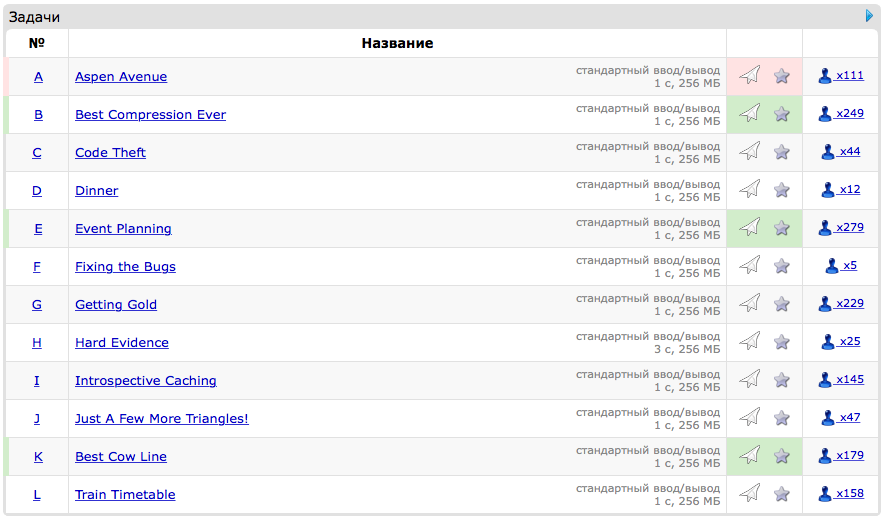
\includegraphics[width=0.95\textwidth]{CT_S02E03/CT_S02E03_result.png}\\ [1cm]
\end{center}

\textbf{{\large Ссылка на контест: \url{http://codeforces.com/gym/100494}}}

\newpage
\textbf{{\large Задача B - Best Compression Ever}}

\begin{center}
%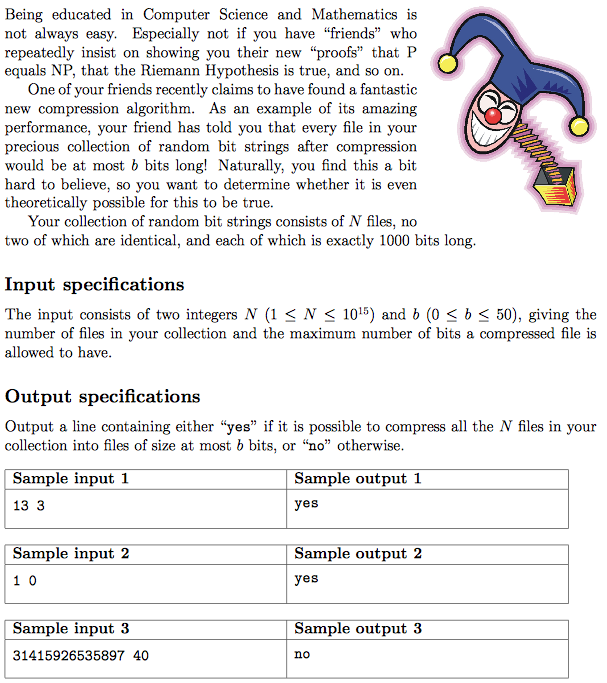
\includegraphics[width=0.9\textwidth]{CT_S02E03/CT_S02E03_B.png}\\ [1cm]
\end{center}

\textbf{{\large Алгоритм}}

Решение довольно простое. Можно заметить, что если логарифм по основаню 2 числа n меньше или равен b, то ответ yes, иначе ответ no. Cложность $O(1)$.

\newpage
\textbf{{\large Исходный код}} \\
\begin{lstlisting}[language=C]
#include <iostream>
#include <cmath>

using namespace std;

int main() {
    ios_base::sync_with_stdio(false);
    
    unsigned long long n;
    int b;
    cin >> n >> b;
    
    if ((int)log2((double)n) <= b) {
        cout << "yes" << endl;
    }
    else {
        cout << "no" << endl;
    }

    return 0;
}
\end{lstlisting}


\newpage
\textbf{{\large Задача E - Event Planning}}

\begin{center}
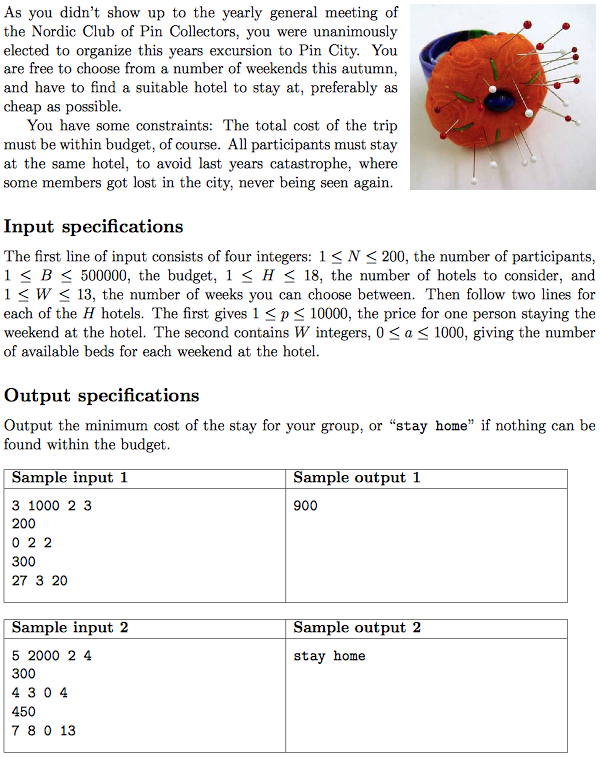
\includegraphics[width=0.9\textwidth]{CT_S02E03/CT_S02E03_E.png}\\ [1cm]
\end{center}

\textbf{{\large Алгоритм}}

Перебираем все отели и все выходные дни, находим самое выгодное предложение, которое соответствует условиям $N * p <= B$ и $a >= N$. Сложность $O(H*W)$, где $H$ - количество отелей, а $W$ - количество недель.

\newpage
\textbf{{\large Исходный код}} \\
\begin{lstlisting}[language=C]
#include <iostream>
#include <vector>

#define ll long long
using namespace std;

int main () {
    ll N,B,H,W,p,a;
    ll min_cost = 5000000;

    cin >> N >> B >> H >> W;

    for (ll i = 0; i < H; i++) {
        cin >> p;
            for (ll k = 0; k < W; k++) {
                cin >> a;
                if((a >= N) && (p * N <= B) && (p * N <= min_cost))
                    min_cost = p * N;
            }
    }
    if(min_cost < 5000000)
        cout << min_cost << endl;
    else cout << "stay home" << endl;


    return 0;
}
\end{lstlisting}


\newpage
\textbf{{\large Задача K - Best Cow Line}}

\begin{center}
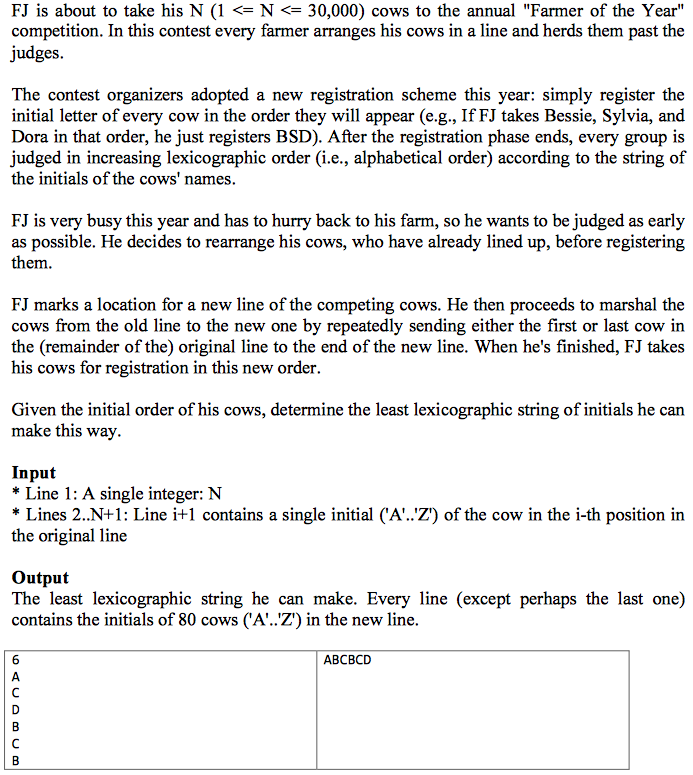
\includegraphics[width=0.9\textwidth]{CT_S02E03/CT_S02E03_K.png}\\ [1cm]
\end{center}

\textbf{{\large Алгоритм}}

Для решения этой задачи нужно чтобы построить последовательность букв по заданным правилам. Будем смотреть на первую и последнюю буквы и брать лексикографически наименьшую. Если буквы совпадают, то надо посмотреть следующие буквы до первого несовпадения и взять букву с той стороны, с которой несовпавшая буква оказалась лексикографически меньше. Сложность $O(n)$.


\newpage
\textbf{{\large Исходный код}} \\
\begin{lstlisting}[language=C]
#include <iostream>
#include <cmath>
#include <vector>
#include <stack>
#include <algorithm>

using namespace std;

int main() {
    int n;
    cin >> n;
    vector<char> cows(n);
    char symb;
    
    for (int i = 0; i < n; i++) {
        cin >> symb;
        cows[i] = symb;
    }
    
    vector<char> newLine;
    int cowsInOldLine = n;
    int begin = 0;
    int end   = n - 1;
    int tempBegin = begin;
    int tempEnd   = end;
    
    while (cowsInOldLine) {
        tempBegin = begin;
        tempEnd   = end;
        if (cows[begin] == cows[end]) {
            while (cows[tempBegin] == cows[tempEnd]) {
                tempBegin++;
                tempEnd--;
                if (tempBegin > tempEnd || tempBegin == tempEnd) {
                    tempBegin = begin;
                    tempEnd = end;
                    break;
                }
            }
        }
        if (cows[tempBegin] < cows[tempEnd]) {
            newLine.push_back(cows[begin]);
            begin++;
        }
        else {
            newLine.push_back(cows[end]);
            end--;
        }
        cowsInOldLine--;
    }
    for (int i = 0; i < n; i++) {
        cout << newLine[i];
        if ((i + 1) % 80 == 0) cout << endl;
    }
    cout << endl;
    return 0;
}
\end{lstlisting}



%----------------------------------------------------------------------------------------
%
%	Codeforces Training S02E04
%
%----------------------------------------------------------------------------------------
\newpage
\subsection{Codeforces Training S02E04}

\textbf{{\large Результаты}} \\
\begin{center}
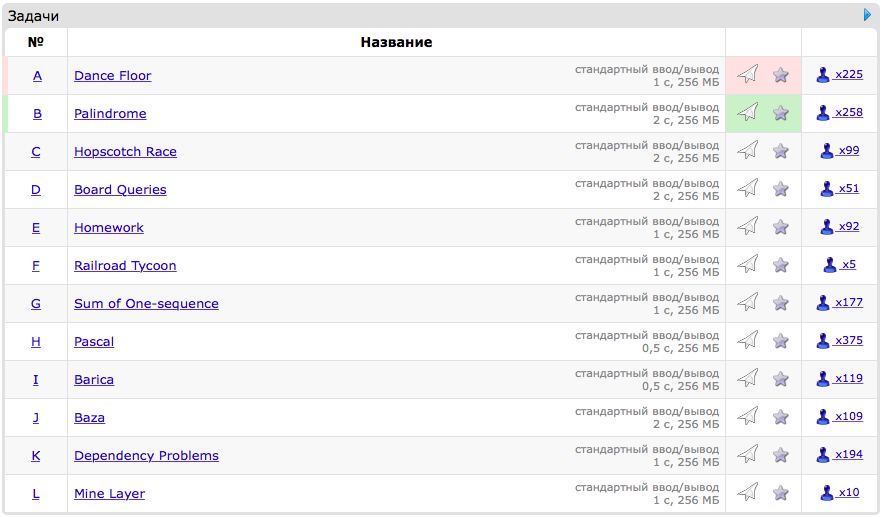
\includegraphics[width=0.95\textwidth]{CT_S02E04/CT_S02E04_result.png}\\ [1cm]
\end{center}

\textbf{{\large Ссылка на контест: \url{http://codeforces.com/gym/100497}}}


\newpage
\textbf{{\large Задача B - Palindrome}} \\

Manao and his friend like to ask each other brainteasers every other day. Recently, Manao's friend brought him a string s and claimed this string has been obtained from a palindrome (see notes for definition of palindrome) by picking two positions and exchanging characters at those positions. The friend asked Manao to determine the palindrome that the string was obtained from. \\

Manao suspects his friend could have cheated and the string could not be a result of the abovementioned process. Also, he noticed that there might be several possible answers to the problem posed. Help him out by finding all the possible answers, or determining that there is none. \\

\textbf{Input} \\
The single line contains the string s consisting of
at least 2 characters. The string will contain lowercase letters only. The length of the string will not exceed 100000. \\

\textbf{Output} \\
In the first line, print a single number p - the number of different palindromes from which the given string can be obtained by exchanging letters at exactly two positions. Print these palindromes in the next p lines, one answer per line. The palindromes should be ordered lexicographically. \\

\textbf{Samples} 

\begin{table}[ht!]
\centering
%\caption{My caption}
\label{my-tab100}
\begin{tabular}{|l|l|}
\hline

abab & 2 \\ & abba \\ & baab \\ \hline
abracacarba & 1 \\ & abracacarba \\ \hline

% Строки таблицы
\end{tabular}
\end{table}

\textbf{{\large Алгоритм}}

Находим буквы, при замене которых получается палиндром и проверяем сколько можно составить палиндромов из этой строки. Всего возможно три варианта: $0, 1, 2$. Сложность $O(n)$.

\newpage
\textbf{{\large Исходный код}} \\
\begin{lstlisting}[language=C]
#include <iostream>
#include <cstdio>
#include <cstring>
using namespace std;

int main(int argc, const char * argv[]) {
    char str[100001];
    int n=0;
    while((str[n++]=getchar())!='\n');
    str[--n]='\0';
    int bad_c1 = -1, bad_c2 = -1;
    for(int i=0; i<n/2; ++i)
    {
        if(str[i]!=str[n-i-1])
        {
            bad_c1 = i;
            bad_c2 = n-i-1;
            break;
        }
    }
    if(bad_c1==-1)
    {
        cout << "1\n" << str << endl;
        return 0;
    }
    char pali1[100001], pali2[100001];
    for(int i=0; i<n; ++i)
    {
        if(i==bad_c1 || i==bad_c2)
            continue;
        if(str[bad_c1]==str[n-i-1] && str[i]==str[bad_c2])
        {
            for(int j=0; j<n; ++j)
            {
                pali1[j]=str[j];
                pali2[j]=str[j];
            }
            pali1[bad_c1]=str[i];
            pali1[i]=str[bad_c1];
            
            pali2[bad_c2]=str[n-i-1];
            pali2[n-i-1]=str[bad_c2];
            bool f1=0, f2=0;
            for(int j=0; j<n/2; ++j)
                if(pali1[j]!=pali1[n-j-1])
                {
                    f1=1;
                    break;
                }
            for(int j=0; j<n/2; ++j)
                if(pali2[j]!=pali2[n-j-1])
                {
                    f2=1;
                    break;
                }
            if(f1&&f2)
            {
                cout << "0\n";
                return 0;
            }
            else if(f1)
            {
                cout << "2\n" << pali2 << '\n';
                return 0;
            }
            else if(f2)
            {
                cout << "1\n" << pali1 << '\n';
                return 0;
            }
            else
            {
                cout << "2\n";
                if(strcmp(pali1, pali2)<0)
                    cout << pali1 << '\n' << pali2;
                else
                    cout << pali2 << '\n' << pali1;
            }
            return 0;
            
        }
    }
    for(int i=0; i<n; ++i)
    {
        if(str[bad_c1]==str[n-i-1])
        {
            for(int j=0; j<n; ++j)
            {
                pali1[j]=str[j];
            }
            pali1[bad_c2]=str[n-i-1];
            pali1[n-i-1]=str[bad_c2];
            bool f=0;
            for(int j=0; j<n/2; ++j)
                if(pali1[j]!=pali1[n-j-1])
                {
                    f=1;
                    break;
                }
            if(f)
                continue;
            cout << "1\n" << pali1 << '\n';
            return 0;
        }
        else if(str[i]==str[bad_c2])
        {
            for(int j=0; j<n; ++j)
            {
                pali2[j]=str[j];
            }
            pali2[bad_c1]=str[i];
            pali2[i]=str[bad_c1];
            bool f=0;
            for(int j=0; j<n/2; ++j)
                if(pali2[j]!=pali2[n-j-1])
                {
                    f=1;
                    break;
                }
            if(f)
                continue;
            cout << "1\n" << pali2 << '\n';
            return 0;
        }
    }
    cout << "0\n";
    return 0;
}
\end{lstlisting}



%----------------------------------------------------------------------------------------
%
%	XV Открытая Всесибирская олимпиада по программированию им И.В. Поттосина
%
%----------------------------------------------------------------------------------------

\newpage
\subsection{XV Открытая Всесибирская олимпиада по программированию им И.В. Поттосина}

\textbf{{\large Результаты}} \\
\begin{center}
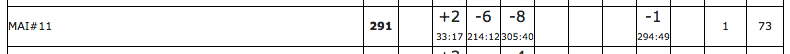
\includegraphics[width=0.95\textwidth]{Siberia/Siberia_result.png}\\ [1cm]
\end{center}

\textbf{{\large Ссылка на контест: \url{https://olympic.nsu.ru/nsuts-new/news.cgi}}}

\newpage
\textbf{{\large Задача 2 - Копировальный аппарат}}

\begin{center}
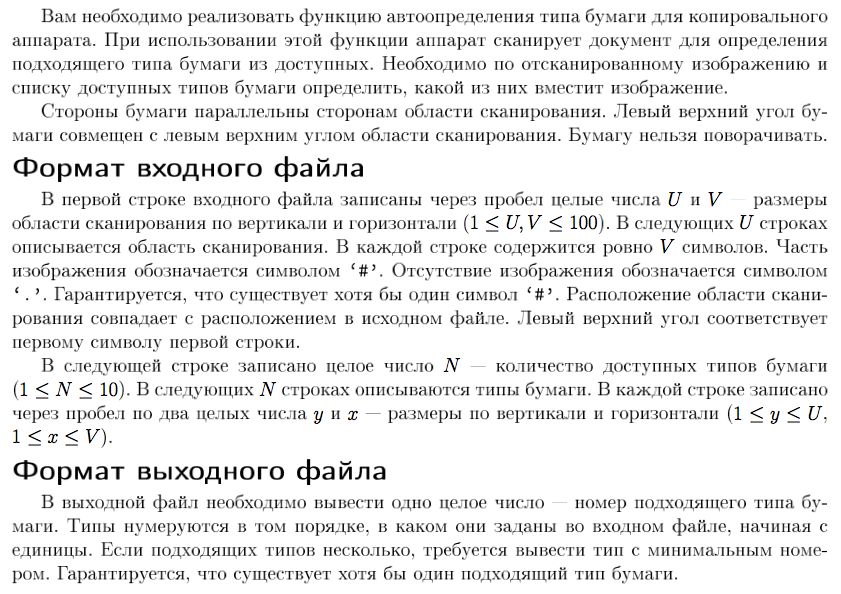
\includegraphics[width=0.9\textwidth]{Siberia/Siberia_1.png}\\ [1cm]
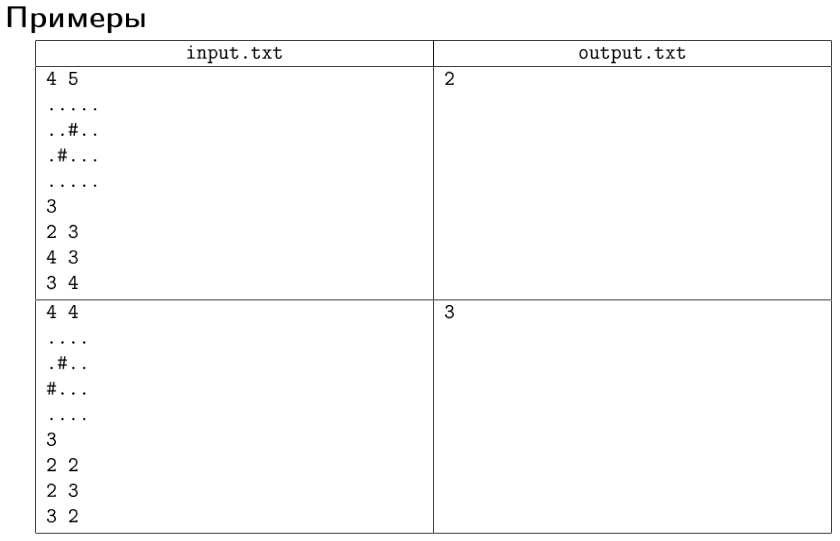
\includegraphics[width=0.6\textwidth]{Siberia/Siberia_2.png}\\ [1cm]
\end{center}

\textbf{{\large Алгоритм}}

Задача на реализацию. Нужно считать входные данные в двумерный массив символов, затем пройтись по всем элементам и запомнить наибольшие позиции, на которых находятся решетки.

\newpage
\textbf{{\large Исходный код}} \\
\begin{lstlisting}[language=C]
#include <iostream>
#include <algorithm>
#include <cmath>

#include <sstream>
#include <fstream>

#define LL  long long

using namespace std;

int main() {
    ifstream in;
    ofstream out;
    in.open("input.txt");
    out.open("output.txt");
    
    LL a, b;
    in >> a >> b;
    char pic[a + 1][b + 1];
    LL XMax = 0;
    LL YMax = 0;
    
    for (LL i = 1; i <= a; i++) {
        for (LL j = 1; j <= b; j++) {
            in >> pic[i][j];
            if (pic[i][j] == '#' && j > XMax) XMax = j;
            if (pic[i][j] == '#' && i > YMax) YMax = i;
        }
        in.get();
    }
    LL n, y, x;
    in >> n;
    for (LL i = 1; i <= n; i++) {
        in >> y >> x;
        if (y >= YMax && x >= XMax) {
            out << i << endl;
            return 0;
        }
    }
    in.close();
    out.close();
    
    return 0;
}
\end{lstlisting}



%----------------------------------------------------------------------------------------
%
%	Codeforces Training S02E05
%
%----------------------------------------------------------------------------------------

\newpage
\subsection{Codeforces Training S02E05}

\textbf{{\large Результаты}} \\
\begin{center}
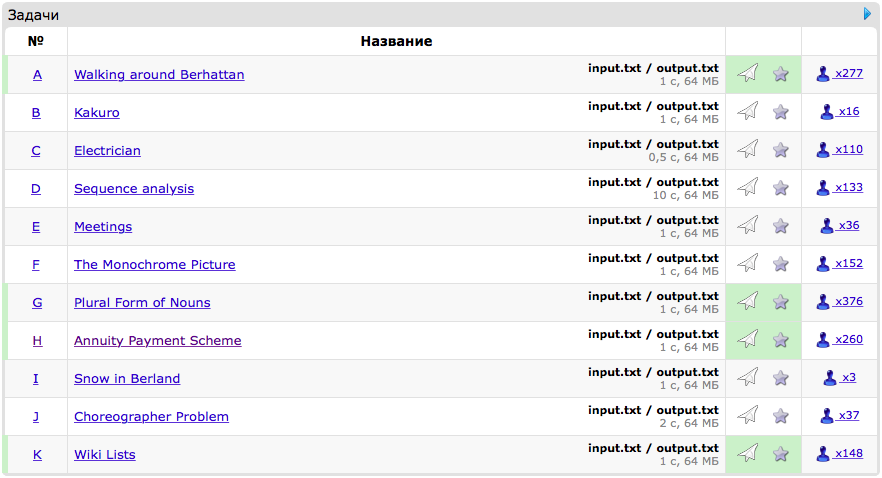
\includegraphics[width=0.95\textwidth]{CT_S02E05/CT_S02E05_result.png}\\ [1cm]
\end{center}

\textbf{{\large Ссылка на контест: \url{http://codeforces.com/gym/100503}}}

\newpage
\textbf{{\large Задача A - Walking around Berhattan}}

\begin{center}
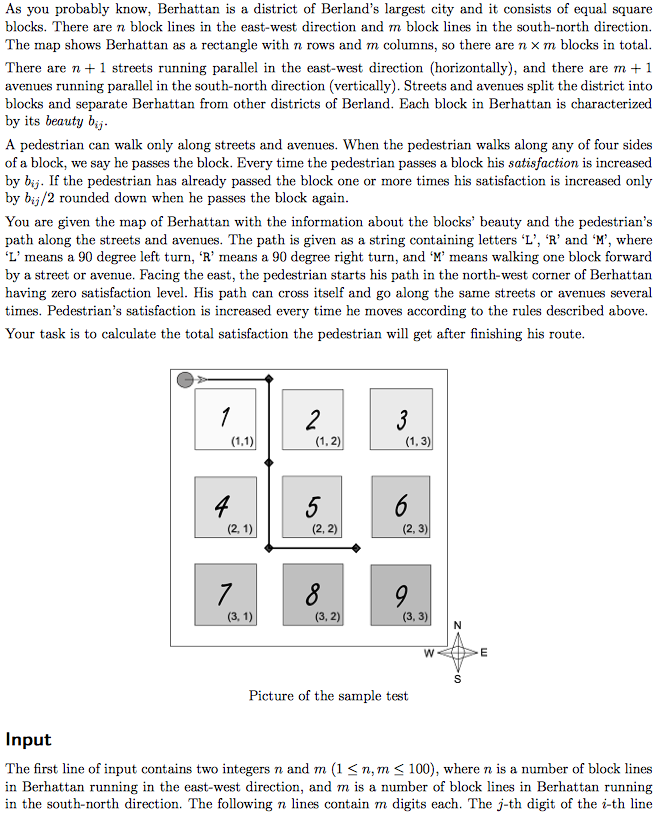
\includegraphics[width=0.9\textwidth]{CT_S02E05/CT_S02E05_A1.png}\\ [1cm]
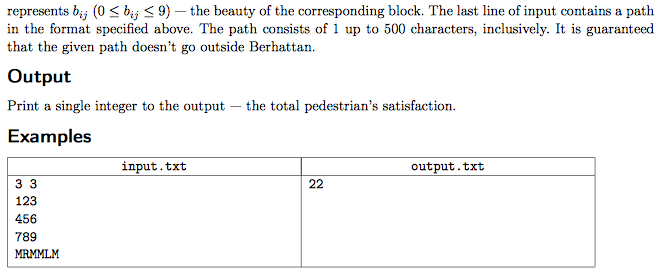
\includegraphics[width=0.9\textwidth]{CT_S02E05/CT_S02E05_A2.png}\\ [1cm]
\end{center}

\textbf{{\large Алгоритм}}

Задача на реализацию. Нужно построить матрицу заданного размера и симулировать передвижение между элементами, записывая изменения. Сложность алгоритма $O(nm)$. \\

\textbf{{\large Исходный код}} \\
\begin{lstlisting}[language=C]
#include <iostream>
#include <algorithm>
#include <iomanip>
#include <vector>
#include <sstream>
#include <fstream>
#define LL  long long

using namespace std;

enum dtype {
    UP,
    DOWN,
    LEFT,
    RIGHT,
};

int main() {
    ifstream in;
    ofstream out;
    in.open("input.txt");
    out.open("output.txt");

    LL n, m;
    LL answer = 0;
    in >> n >> m;
    char t;
    in.get();
    
    vector< vector<int> > map(n + 2, vector<int>(m + 2, 0));
    vector< vector<bool> > used(n + 2, vector<bool>(m + 2, false));
    
    for (LL i = 1; i <= n; i++) {
        for (LL j = 1; j <= m; j++) {
            t = in.get();
            map[i][j] = t - '0';
        }
        in.get();
    }
    
    int x = 1, y = 1;
    dtype dir = RIGHT; // last dir

    while ((t = in.get()) != EOF) {
        if (t == 'M') {
            if (dir == RIGHT) {
 				answer += map[x][y];
                answer += map[x - 1][y];
            	if (!used[x][y]) {
                	map[x][y] /= 2;
                	used[x][y] = true;
                }
                if (!used[x - 1][y]) {
                	map[x - 1][y] /= 2;
                	used[x - 1][y] = true;
                }
                y++;
            }
            else if (dir == LEFT) {
            	answer += map[x][y - 1];
                answer += map[x - 1][y - 1];
            	if (!used[x][y - 1]) {
            		map[x][y - 1] /= 2;
            		used[x][y - 1] = true;
            	}
            	if (!used[x - 1][y - 1]) {
            		map[x - 1][y - 1] /= 2;
                	used[x - 1][y - 1] = true;
            	}
                y--;
            }
            else if (dir == UP) {
                answer += map[x - 1][y - 1];
                answer += map[x - 1][y];
                if (!used[x - 1][y - 1]) {
                	map[x - 1][y - 1] /= 2;
                	used[x - 1][y - 1] = true;
                }
                if (!used[x - 1][y]) {
                	map[x - 1][y] /= 2;
                	used[x - 1][y] = true;
                }
                x--;
            }
            else if (dir == DOWN) {
                answer += map[x][y];
                answer += map[x][y - 1];
                if (!used[x][y]) {
                	map[x][y] /= 2;
                	used[x][y] = true;
                }
                if (!used[x][y - 1]) {
                	map[x][y - 1] /= 2;
               		used[x][y - 1] = true;
                }
                x++;
            }
            
        }
        else if (t == 'R') {
            if (dir == UP) dir = RIGHT;
            else if (dir == DOWN) dir = LEFT;
            else if (dir == LEFT) dir = UP;
            else dir = DOWN;
        }
        else if (t == 'L'){
            if (dir == UP) dir = LEFT;
            else if (dir == DOWN) dir = RIGHT;
            else if (dir == LEFT) dir = DOWN;
            else dir = UP;
        }
    }
    out << answer << endl;
    in.close();
    out.close();
    return 0;
}
\end{lstlisting}


\newpage
\textbf{{\large Задача G - Plural Form of Nouns}}

\begin{center}
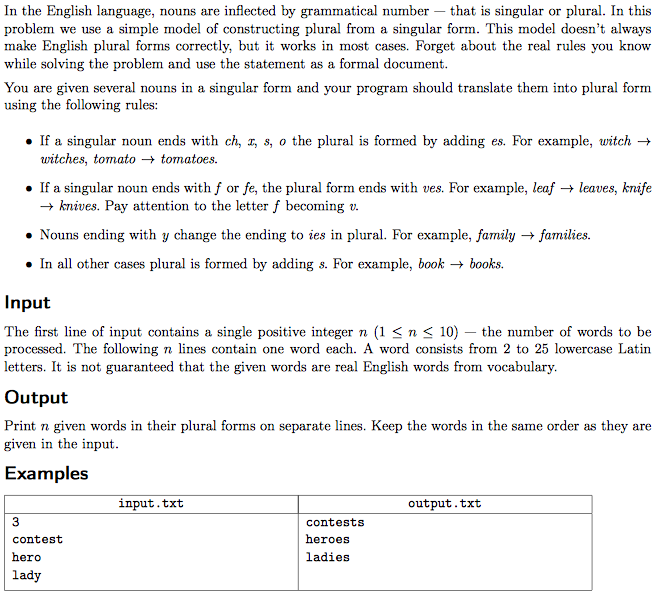
\includegraphics[width=0.9\textwidth]{CT_S02E05/CT_S02E05_G.png}\\ [1cm]
\end{center}

\textbf{{\large Алгоритм}}

Задача на реализацию. Нужно считать слова и в зависимости от окончания изменить его на нужное. Сложность $O(n)$.

\newpage
\textbf{{\large Исходный код}} \\
\begin{lstlisting}[language=C]
#include <iostream>
#include <sstream>
#include <fstream>
#define LL  long long

using namespace std;

int main() {
    ifstream in;
    ofstream out;
    in.open("input.txt");
    out.open("output.txt");

    LL n;
    string s;
    
    in >> n;
    
    for (LL i = 0; i < n; i++) {
        in >> s;
        size_t l = s.size() - 1;
        if ((s[l] == 'h' && s[l - 1] == 'c') || s[l] == 's' || s[l] == 'x' || s[l] == 'o') {
            out << s;
            out << "es" << endl;
        }
        else if (s[l] == 'f') {
            for (size_t j = 0; j < l; j++) {
                out << s[j];
            }
            out << "ves" << endl;
        }
        else if (s[l] == 'e' && s[l - 1] == 'f') {
            for (size_t j = 0; j < l - 1; j++) {
                out << s[j];
            }
            out << "ves" << endl;
        }
        else if (s[l] == 'y') {
            for (size_t j = 0; j < l; j++) {
                out << s[j];
            }
            out << "ies" << endl;
        }
        else {
            out << s << "s" << endl;
        }
    }
    
    in.close();
    out.close();
    
    return 0;
}
\end{lstlisting}

\newpage
\textbf{{\large Задача H - Annuity Payment Scheme}}

\begin{center}
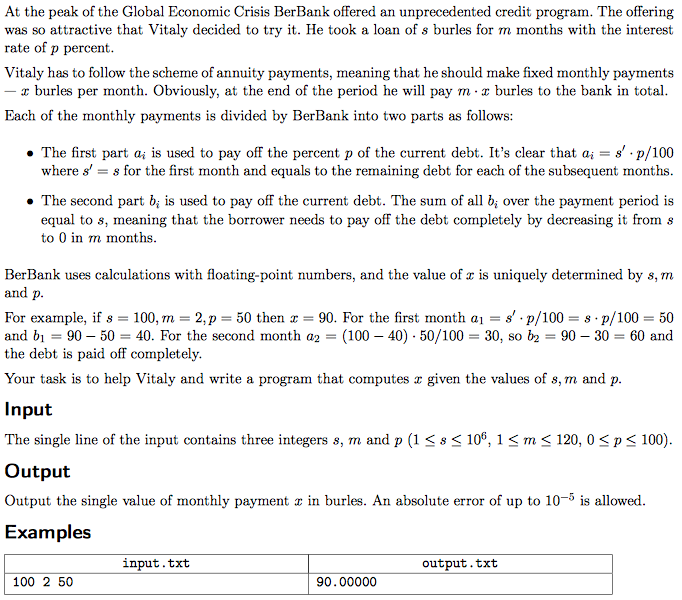
\includegraphics[width=0.9\textwidth]{CT_S02E05/CT_S02E05_H.png}\\ [1cm]
\end{center}

\textbf{{\large Алгоритм}}

Формула для решения задачи выводится из бинома ньютона. Сложность $O(n^2)$. \\

\textbf{{\large Исходный код}} \\
\begin{lstlisting}[language=C]
#include <iostream>
#include <iomanip>
#include <cmath>
#include <fstream>
using namespace std;

int main(int argc, const char * argv[]) {
    double s, p;
    int m;
    ifstream in("input.txt");
    ofstream out("output.txt");
    in >> s >> m >> p;
    if(!p)
    {
        out << fixed;
        out << setprecision(6);
        out << s/(double)m << endl;
        return 0;
    }
    double num;
    double den;
    double binom[300];
    binom[0] = 1;
    double temp1 = 1, temp2=1;
    for(unsigned long i=2; i<=m; ++i)
    {
        temp2 = binom[0];
        for(unsigned long j=1; j<( ((i+2)/2) - ((i%2)?0:1)); ++j)
        {
            temp1 = binom[j];
            binom[j] = temp2+binom[j];            temp2 = temp1;
        }
        if(!(i%2))
        {
            binom[(i+2)/2-1]=temp2*2;
        }
    }
    for(int i=(m+3)/2-1, j=(m+2)/2-1; j>=0; ++i, --j)
        binom[i] = binom[j];
    p /= 100.0;
    num = 0;
    for(int i=0; i<=m; ++i)
    {
        num += binom[i]*pow(p, i);
    }
    den = binom[1];
    for(int i=1; i<m; ++i)
    {
        den += binom[i+1]*pow(p, i);
    }
    double x = num/den*s;
    out << fixed;
    out << setprecision(6);
    out << x << endl;
    in.close();
    out.close();
    return 0;
}
\end{lstlisting}

\newpage
\textbf{{\large Задача K - Wiki Lists}}

\begin{center}
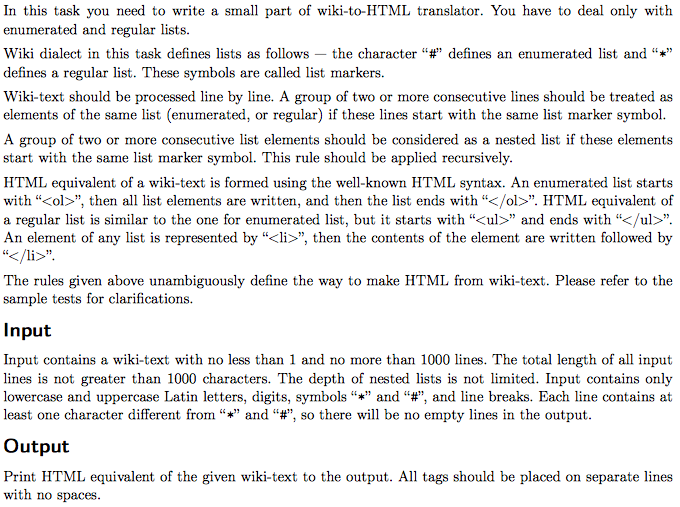
\includegraphics[width=0.9\textwidth]{CT_S02E05/CT_S02E05_K1.png}\\ [1cm]
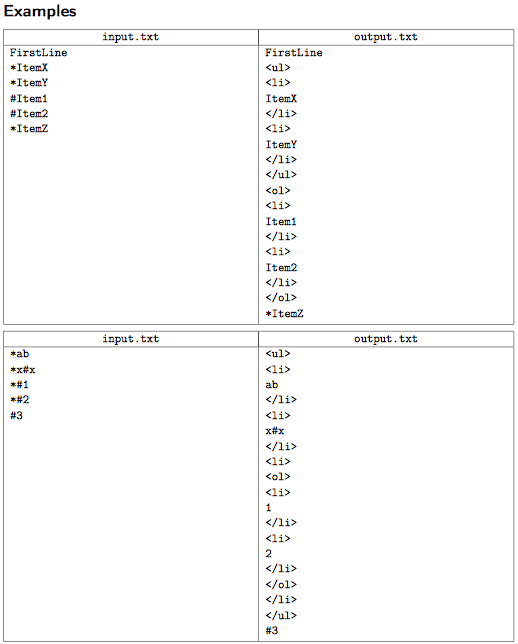
\includegraphics[width=0.9\textwidth]{CT_S02E05/CT_S02E05_K2.png}\\ [1cm]
\end{center}

\textbf{{\large Алгоритм}}

Задача решается с помощью рекурсии. Сложность $O(n)$. \\

\textbf{{\large Исходный код}} \\
\begin{lstlisting}[language=C]
#include <iostream>
#include <fstream>
using namespace std;
//#define out cout
//#define in cin
ifstream in("input.txt");
ofstream out("output.txt");
void func(char **m, int beg, int end, int d, bool list, char sep)
{
    char c = 0;
    int l=0, r=0;
    for(int i=beg; i<=end; ++i)
    {
        if(m[i][d]=='*')
        {
            if(!c)
            {
                c = '*';
                l = i;
                r = i;
            }
            else if(c == '*')
            {
                r = i;
            }
            else if(c == '#')
            {
                if(list)
                    out << "<li>" << sep;
                if(r-l>0)
                {
                    out << "<ol>" << sep;
                    func(m, l, r, d+1, true, sep);
                    out << "</ol>";
                    if(r!=end || d)
                        out.put(sep);
                }
                else
                {
                    out << &m[r][d] << sep;
                }
                if(list)
                    out << "</li>" << sep;
                c = '*';
                l = i;
                r = i;
            }
        }
        else if(m[i][d]=='#')
        {
            if(!c)
            {
                c = '#';
                l = i;
                r = i;
            }
            else if(c == '#')
            {
                r = i;
            }
            else if(c == '*')
            {
                if(list)
                    out << "<li>" << sep;
                if(r-l>0)
                {
                    out << "<ul>" << sep;
                    func(m, l, r, d+1, true, sep);
                    out << "</ul>";
                    if(r!=end || d)
                        out.put(sep);
                }
                else
                {
                    out << &m[r][d] << sep;
                }
                if(list)
                    out << "</li>" << sep;
                c = '#';
                l = i;
                r = i;
            }
        }
        else
        {
            if(c)
            {
                if(list)
                    out << "<li>" << sep;
                if(r-l>0)
                {
                    if(c == '*')
                    {
                        out << "<ul>" << sep;
                        func(m, l, r, d+1, true, sep);
                        out << "</ul>";
                        if(r!=end || d)
                            out.put(sep);
                    }
                    if(c == '#')
                    {
                        out << "<ol>" << sep;
                        func(m, l, r, d+1, true, sep);
                        out << "</ol>";
                        if(r!=end || d)
                            out.put(sep);
                    }
                }
                else
                {
                    out << &m[r][d] << sep;
                }
                if(list)
                    out << "</li>" << sep;
            }
            r = i;
            l = i;
            c = 0;
            if(list)
                out << "<li>" << sep;
            out << &m[i][d];
            if(r!=end || d)
                out.put(sep);
            if(list)
                out << "</li>" << sep;
        }
    }
    if(!c)
        return;
    if(list)
        out << "<li>" << sep;
    if(r-l>0)
    {
        if(c == '*')
        {
            out << "<ul>" << sep;
            func(m, l, r, d+1, true, sep);
            out << "</ul>";
            if(d)
                out.put(sep);
        }
        if(c == '#')
        {
            out << "<ol>" << sep;
            func(m, l, r, d+1, true, sep);
            out << "</ol>";
            if(d)
                out.put(sep);
        }
    }
    else
    {
        out << &m[r][d];
        if(d)
            out.put(sep);
    }
    if(list)
        out << "</li>" << sep;
}
int main(int argc, const char * argv[]) {
    char **m=new char*[1001];
    for(int i=0; i<1001; ++i)
        m[i]=new char[1001];
    int n=0;
    char sep=0;
    while(!in.eof())
    {
        int j=0;
        while(!in.eof() && (m[n][j]=in.get())!=' ' && m[n][j]!='\n') ++j;
        if(in.eof())
            --j;
        if(!sep)
            sep = m[n][j];
        m[n][j] = '\0';
        if(*m[n]!='\0')
            ++n;
    }
    func(m, 0, n-1, 0, false, sep);
    in.close();
    out.close();
    return 0;
}
\end{lstlisting}



%----------------------------------------------------------------------------------------
%
%	Codeforces Training S02E06
%
%----------------------------------------------------------------------------------------
\newpage
\subsection{Codeforces Training S02E06}

\textbf{{\large Результаты}} \\
\begin{center}
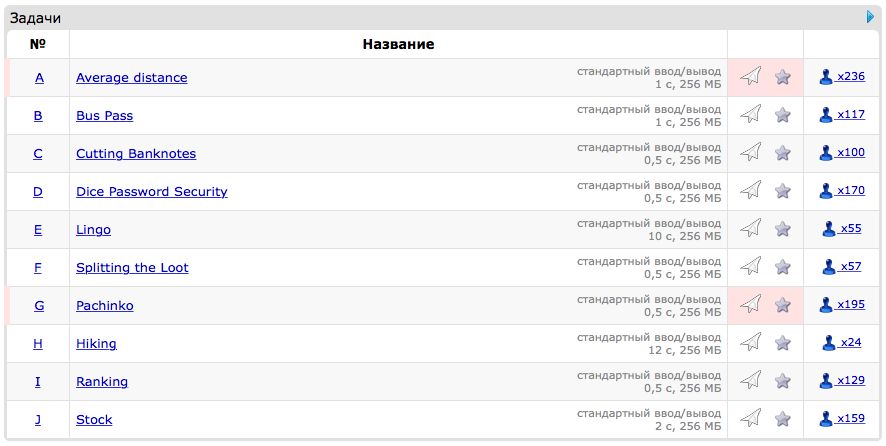
\includegraphics[width=0.95\textwidth]{CT_S02E06/CT_S02E06_result.png}\\ [1cm]
\end{center}

\textbf{{\large Ссылка на контест: \url{http://codeforces.com/gym/100506}}}

%----------------------------------------------------------------------------------------
%
%	Тренировка СПбГУ B #3 Поиск кратчайшего пути и DFS
%
%----------------------------------------------------------------------------------------
\newpage
\subsection{Тренировка СПбГУ Поиск кратчайшего пути и DFS}

\textbf{{\large Результаты}} \\
\begin{center}
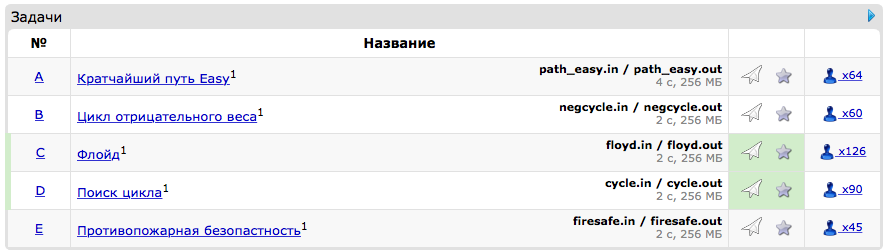
\includegraphics[width=0.95\textwidth]{SPBGU_GRAPHS/SPBGU_GRAPHS_result.png}\\ [1cm]
\end{center}

\textbf{{\large Ссылка на контест: \url{http://codeforces.com/gym/100232}}}

\newpage
\textbf{{\large Задача C - Флойд}} \\
\begin{center}
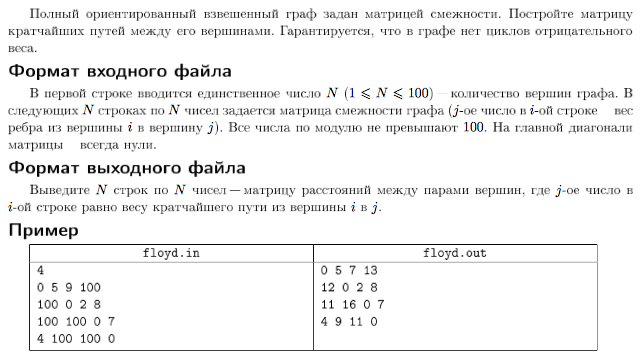
\includegraphics[width=0.9\textwidth]{SPBGU_GRAPHS/SPBGU_GRAPHS_C.png}\\ [1cm]
\end{center}
\textbf{{\large Алгоритм}} \\
В задаче требуется найти кратчайшие пути между всеми парами вершин и представить их матрицей смежности. Ее можно решить используя алгоритм Флойда-Уоршелла за $O(n^3)$. \\ 
\\
\newpage
\textbf{{\large Исходный код}}
\begin{lstlisting}[language=C]
#include <iomanip>
#include <iostream>
#include <algorithm>
#include <fstream>

using namespace std;

int main() {
    
    more_speed
    ifstream in("floyd.in");
    ofstream out("floyd.out");
    
    int n;
    in >> n;
    vector<vector<int> > m(n, vector<int>(n, 0));
    for (int i = 0; i < n; i++) {
        for (int j = 0; j < n; j++) {
            in >> m[i][j];
        }
    }
    
    for (int k = 0; k < n; k++) {
        for (int i = 0; i < n; i++) {
            for (int j = 0; j < n; j++) {
                m[i][j] = min(m[i][j], m[i][k] + m[k][j]);
            }
        }
    }
    
    for (int i = 0; i < n; i++) {
        for (int j = 0; j < n; j++) {
            out << m[i][j];
            if (j < n - 1) out << " ";
            else out << endl;
        }
    }

    in.close();
    out.close();
    
    return 0;
}
\end{lstlisting}


\newpage
\textbf{{\large Задача D - Поиск цикла}} \\
\begin{center}
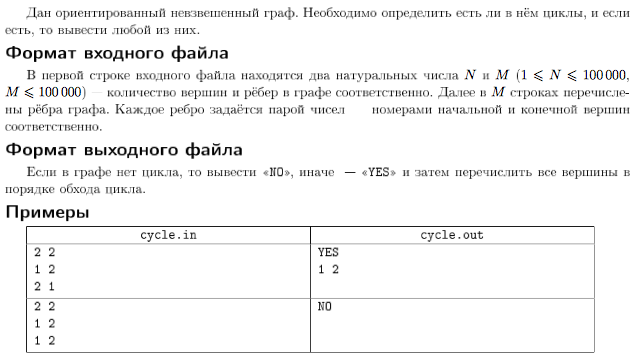
\includegraphics[width=0.9\textwidth]{SPBGU_GRAPHS/SPBGU_GRAPHS_D.png}\\ [1cm]
\end{center}
\textbf{{\large Алгоритм}} \\
Задача решается поиском в глубину. Нужно сделать серию поисков в глубину, заходя в новую вершину будем красить ее в серый цвет, а выходя в черный. Если заходим в серую вершину, то цикл найден. \\
%\newpage
\textbf{{\large Исходный код}} \\
\begin{lstlisting}[language=C]
#include <iomanip>
#include <iostream>
#include <algorithm>
#include <fstream>

vector<set<LL> > g;
vector<char> color;
vector<LL> p;
LL cycle_st, cycle_end;

bool dfs (LL v) {
    color[v] = 1;
    for (set<LL>::iterator i = g[v].begin(); i != g[v].end(); i++) {
        LL to = *i;
        if (color[to] == 0) {
            p[to] = v;
            if (dfs(to)) return true;
        }
        else if (color[to] == 1){
            cycle_st = to;
            cycle_end = v;
            return true;
        }
    }
    color[v] = 2;
    return false;
}

using namespace std;
int main() {
    
    more_speed
    ifstream in("cycle.in");
    ofstream out("cycle.out");
    
    LL n, m, f, t;
    in >> n >> m;
    g.resize(n);
    
    for (LL i = 0; i < m; i++) {
        in >> f >> t;
        g[f - 1].insert(t - 1);
    }
    
    p.assign(n, -1);
    color.assign(n, 0);
    cycle_st = -1;
    for (LL i = 0; i < n; i++) {
        if (dfs(i)) break;
    }
    if (cycle_st == -1) {
        out << "NO" << endl;
    }
    else {
        out << "YES" << endl;
        vector<LL> cycle;
        for (LL v = cycle_end; v != cycle_st; v = p[v]) {
            cycle.push_back(v);
        }
        cycle.push_back(cycle_st);
        reverse(cycle.begin(), cycle.end());
        for (size_t i = 0; i < cycle.size(); i++) {
            out << cycle[i] + 1 << " ";
        }
        out << endl;
    }
    in.close();
    out.close();
    
    return 0;
}
\end{lstlisting}



%----------------------------------------------------------------------------------------
%
%	OpenCup GP of SPb
%
%----------------------------------------------------------------------------------------
\newpage
\subsection{OpenCup GrandPrix of SPb.}

\textbf{{\large Задача А - Барабашка}} \\
\begin{center}
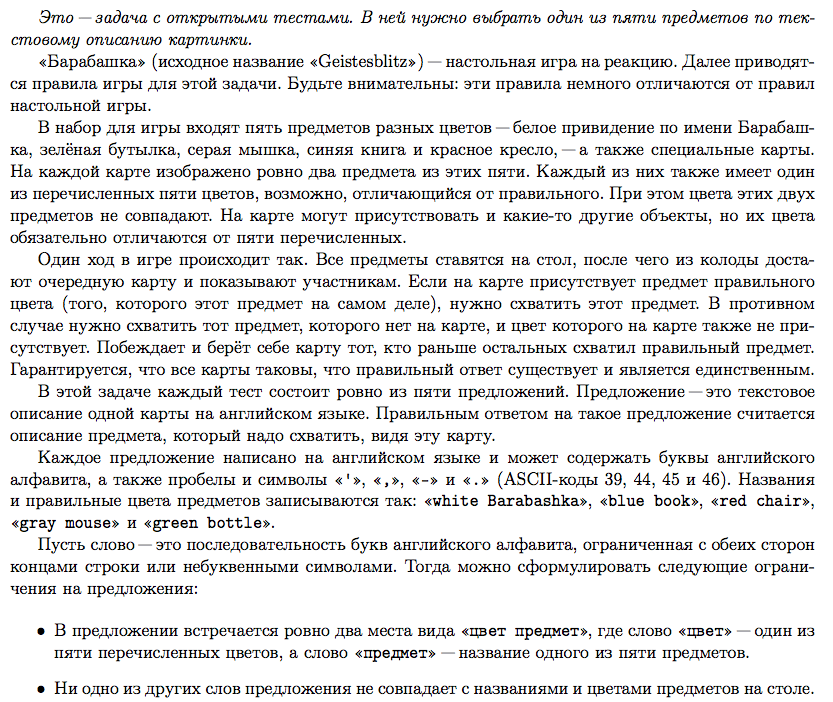
\includegraphics[width=0.9\textwidth]{OC_SPB/OC_SPB_A1.png}\\ [1cm]
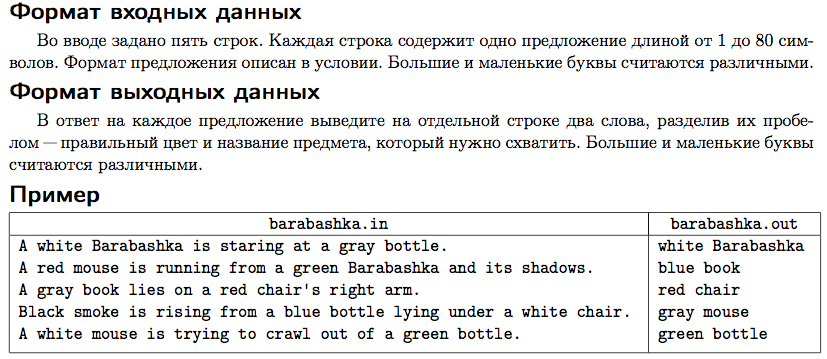
\includegraphics[width=0.9\textwidth]{OC_SPB/OC_SPB_A2.png}\\ [1cm]
\end{center}
\newpage

\textbf{{\large Алгоритм}} \\
Задача на реализацию. Нужно считать строки и каждой строке сопоставить правильное сочетание цвета и предмета по заданым в условии правилам. Сначала определим, какие сочетания уже имеются в предложении, затем проверим, есть ли среди них корректные, если есть, то это ответ, иначе нужно выбрать любое правильное сочетание. \\ 
\\
%\newpage
\textbf{{\large Исходный код}}
\begin{lstlisting}[language=C++]
#include <iomanip>
#include <iostream>
#include <algorithm>

bool isChar(char c) {
    return (c >= 'A' && c <= 'Z') || (c >= 'a' && c <= 'z');
}

int num(string s) {
    if      (s == "white" || s == "barabashka") return 0;
    else if (s == "blue"  || s == "book")       return 1;
    else if (s == "red"   || s == "chair")      return 2;
    else if (s == "gray"  || s == "mouse")      return 3;
    else return 4;
}
 
int main() {
    ifstream in("barabashka.in");
    ofstream out("barabashka.out");
    
    string white = "white",
           blue  = "blue",
           red   = "red",
           gray  = "gray",
           green = "green";
    string barab = "barabashka",
           book  = "book",
           chair = "chair",
           mouse = "mouse",
           bottle = "bottle";
    
    string current;
    string firstColor, firstObject;
    string secondColor, secondObject;
    bool needFirstColor, needFirstObject;
    bool needSecondColor, needSecondObject;
    bool complete;
    
    
    for (int i = 0; i < 5; i++) {
        char cSymb = in.get();
        bool used[5] = {false};
        needFirstColor   = true;
        needFirstObject  = false;
        needSecondColor  = false;
        needSecondObject = false;
        complete         = false;
        
        while (cSymb != '0') {
            while (cSymb != ' ' && isChar(cSymb)) {
                current += tolower(cSymb);
                cSymb = in.get();
            }
            if (needFirstColor) {
                if (current == white)      { firstColor = white; needFirstObject = true; needFirstColor = false; }
                else if (current == blue)  { firstColor = blue;  needFirstObject = true; needFirstColor = false; }
                else if (current == red)   { firstColor = red;   needFirstObject = true; needFirstColor = false; }
                else if (current == gray)  { firstColor = gray;  needFirstObject = true; needFirstColor = false; }
                else if (current == green) { firstColor = green; needFirstObject = true; needFirstColor = false; }
            }
            else if (needFirstObject) {
                if (current == barab)       { firstObject = barab;  needSecondColor = true; needFirstObject = false; }
                else if (current == book)   { firstObject = book;   needSecondColor = true; needFirstObject = false; }
                else if (current == chair)  { firstObject = chair;  needSecondColor = true; needFirstObject = false; }
                else if (current == mouse)  { firstObject = mouse;  needSecondColor = true; needFirstObject = false; }
                else if (current == bottle) { firstObject = bottle; needSecondColor = true; needFirstObject = false; }
            }
            else if (needSecondColor) {
                if (current == white)      { secondColor = white; needSecondObject = true; needSecondColor = false; }
                else if (current == blue)  { secondColor = blue;  needSecondObject = true; needSecondColor = false; }
                else if (current == red)   { secondColor = red;   needSecondObject = true; needSecondColor = false; }
                else if (current == gray)  { secondColor = gray;  needSecondObject = true; needSecondColor = false; }
                else if (current == green) { secondColor = green; needSecondObject = true; needSecondColor = false; }
            }
            else if (needSecondObject) {
                if (current == barab)       { secondObject = barab;  complete = true; needSecondObject = false; }
                else if (current == book)   { secondObject = book;   complete = true; needSecondObject = false; }
                else if (current == chair)  { secondObject = chair;  complete = true; needSecondObject = false; }
                else if (current == mouse)  { secondObject = mouse;  complete = true; needSecondObject = false; }
                else if (current == bottle) { secondObject = bottle; complete = true; needSecondObject = false; }
            }
            if (complete) {
                cSymb = '0';
                used[num(firstColor)] = true;
                used[num(firstObject)] = true;
                used[num(secondColor)] = true;
                used[num(secondObject)] = true;
                
                if ((firstColor == white && firstObject == barab) ||
                    (secondColor == white && secondObject == barab)) { out << white << " " << "Barabashka" << endl; }
                
                else if ((firstColor == blue && firstObject == book) ||
                         (secondColor == blue && secondObject == book)) { out << blue << " " << book << endl; }
                
                else if ((firstColor == red && firstObject == chair) ||
                         (secondColor == red && secondObject == chair)) { out << red << " " << chair << endl; }
                
                else if ((firstColor == gray && firstObject == mouse) ||
                         (secondColor == gray && secondObject == mouse)) { out << gray << " " << mouse << endl; }
                
                else if ((firstColor == green && firstObject == bottle) ||
                         (secondColor == green && secondObject == bottle)) { out << green << " " << bottle << endl; }
                
                else {
                    for (int j = 0; j < 5; j++) {
                        if (!used[j]) {
                            if (j == 0) { out << white << " " << "Barabashka" << endl; }
                            else if (j == 1) { out << blue << " " << book << endl; }
                            else if (j == 2) { out << red << " " << chair << endl; }
                            else if (j == 3) { out << gray << " " << mouse << endl; }
                            else             { out << green << " " << bottle << endl; }
                            break;
                        }
                    }
                }
                
                
            }
            current.clear();
            if (cSymb != '\0') cSymb = in.get();
        }
    }
    return 0;
}
\end{lstlisting}

\textbf{{\large Результаты}} \\
\begin{center}
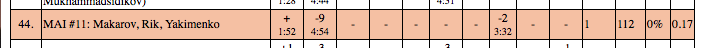
\includegraphics[width=0.95\textwidth]{OC_SPB/OC_SPB_result.png}\\ [1cm]
\end{center}



%----------------------------------------------------------------------------------------
%
%	Самарский Международный Аэрокосмический Лицей, тренировка №1
%
%----------------------------------------------------------------------------------------
\newpage
\subsection{Самарский Международный Аэрокосмический Лицей, тренировка №1}

\textbf{{\large Задача D - Пивной вор}} \\
\begin{center}
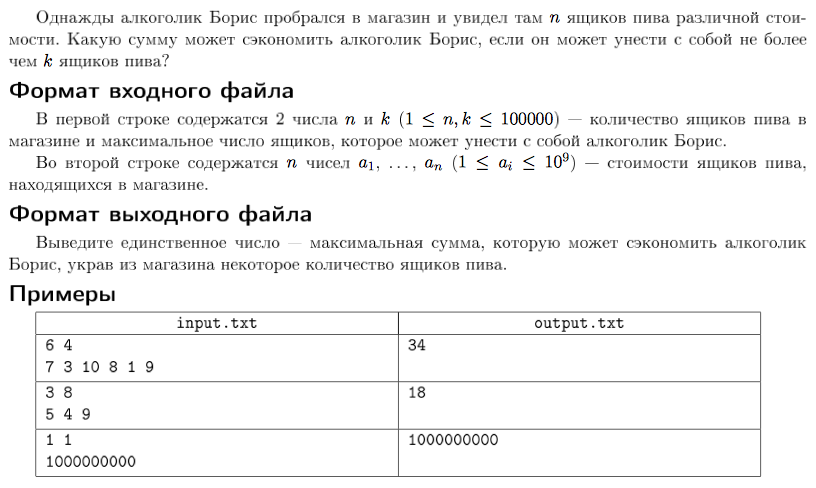
\includegraphics[width=0.9\textwidth]{CT_SAMARA/CT_SAMARA_D.png}\\ [1cm]
\end{center}
\textbf{{\large Алгоритм}} \\
В этой задаче нужно отсортировать массив стоимостей по убыванию и сложить первые $k$ чисел. Это и будет ответом. \\ 
\\
\newpage
\textbf{{\large Исходный код}}
\begin{lstlisting}[language=C]
#include <iostream>
#include <vector>
#include <algorithm>
#include <fstream>

using namespace std;

int main() {
	long n, k;
	ifstream in("input.txt");
	ofstream out("output.txt");
	in >> n >> k;
	vector<long long> v(n);
	for (long i = 0; i < n; i++) {
		in >> v[i];
	}
	sort(v.begin(), v.end(), greater<long long>());
	long long answer = 0;
	for (long i = 0; i < k && i < v.size(); i++) {
		answer += v[i];
	}
	out << answer << endl;
	in.close();
	out.close();
	return 0;
}
\end{lstlisting}

\textbf{{\large Результаты}} \\
\begin{center}
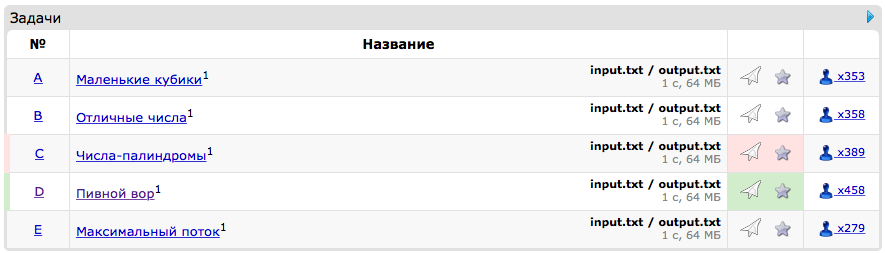
\includegraphics[width=0.95\textwidth]{CT_SAMARA/CT_SAMARA_result.png}\\ [1cm]
\end{center}



%----------------------------------------------------------------------------------------
%
%	Codeforces ACM Восточный четвертьфинал
%
%----------------------------------------------------------------------------------------
\newpage
\subsection{Codeforces ACM-ICPC Восточный четвертьфинал}

\textbf{{\large Задача A - About Grisha N.}} \\
\begin{center}
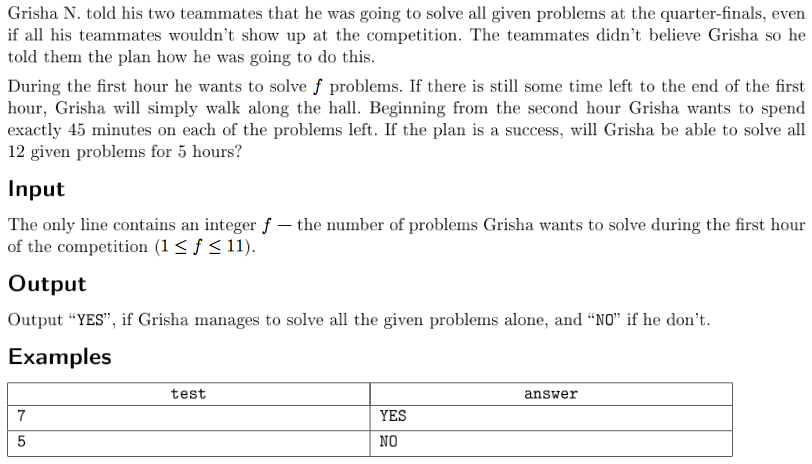
\includegraphics[width=0.9\textwidth]{CT_ACM_EAST/CT_ACM_EAST_A.png}\\ [1cm]
\end{center}
\textbf{{\large Алгоритм}} \\
Для решения задачи достаточно увидеть закономерность, что если $f > 6$, то ответ будет $YES$, иначе ответ будет $NO$. Сложность, очевидно, $O(1)$.\\ 
\\
\textbf{{\large Исходный код}}
\begin{lstlisting}[language=C]
#include <iostream>
using namespace std;

int main(int argc, const char * argv[]) {
    int f;
    cin >> f;
    if(f>6)
        cout << "YES";
    else
        cout << "NO";
    return 0;
}
\end{lstlisting}

\newpage
\textbf{{\large Задача D - Zhenya moves from the dormitory}} \\
\begin{center}
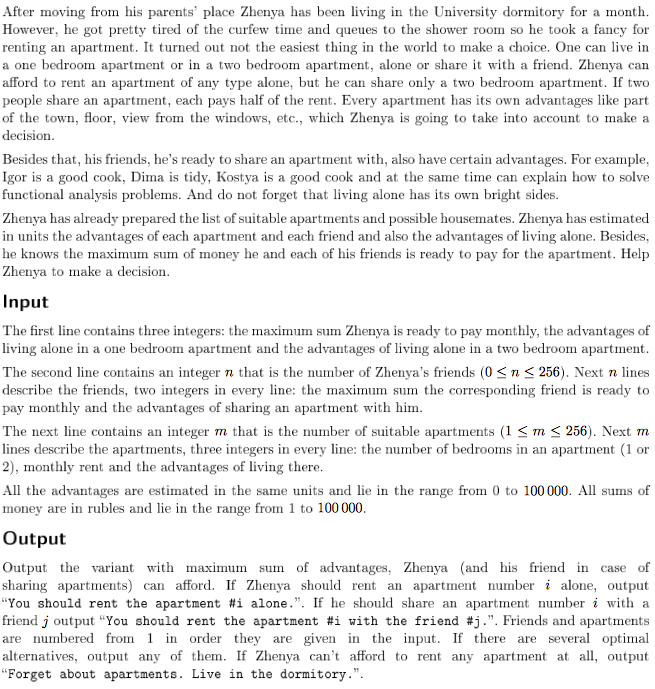
\includegraphics[width=0.9\textwidth]{CT_ACM_EAST/CT_ACM_EAST_D1.png}\\ [1cm]
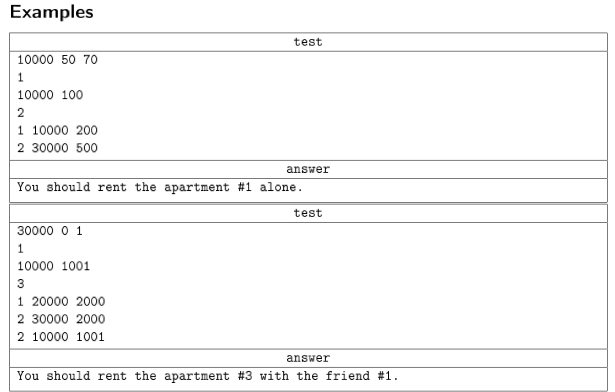
\includegraphics[width=0.5\textwidth]{CT_ACM_EAST/CT_ACM_EAST_D2.png}\\ [1cm]
\end{center}
\textbf{{\large Алгоритм}} \\
Для решения задачи сразу при считывании найдем лучшеие однокомнатные и двухкомнатные квартиры по комфорту, если Женя будет жить один. Затем отсортируем все квартиры по комфорту и для каждого друга Жени будем подбирать лучший вариант при совместной покупке. После этого сравним найденные варианты и выберем лучший. Сложность алгоритма $O(n^2)$.\\
\\
\newpage
\textbf{{\large Исходный код}}
\begin{lstlisting}[language=C]
#include <iostream>
#include <algorithm>
#include <vector>
#include <fstream>

using namespace std;

typedef struct {
    long money;
    long ad;
    int num;
}frd;

typedef struct {
    long rooms;
    long price;
    long ad;
    int num;
}apartment;

bool cmp_ap(const apartment &a1, const apartment &a2) {
    return a1.ad > a2.ad;
}

bool cmp_fr(const frd &f1, const frd &f2) {
    return f1.ad > f2.ad;
}

int find_good_ap(const vector<apartment> &a, long money1, long money2) {
    for (int i = 0; i < a.size(); i++) {
        long price_for_each = a[i].price / 2;
        if (a[i].price % 2 == 1) {
            price_for_each++;
        }
        if (money1 >= price_for_each && money2 >= price_for_each && a[i].rooms == 2)
            return i;
    }
    return -1;
}

int main() {
    long money, ad1, ad2;
    long n, m;
    cin >> money >> ad1 >> ad2;
    cin >> n;
    vector<frd> fr(n);
    for (int i = 0; i < n; i++) {
        cin >> fr[i].money >> fr[i].ad;
        fr[i].num = i + 1;
    }
    cin >> m;
    vector<apartment> ap(m);
    long max_ad_in_1room = -1, max_ad_in_2room = -1;
    int  in_1room_num = -1, in_2room_num = -1;
    bool can_buy_alone = false;
    for (int i = 0; i < m; i++) {
        cin >> ap[i].rooms >> ap[i].price >> ap[i].ad;
        ap[i].num = i + 1;
        if (ap[i].rooms == 1) {
            if (money >= ap[i].price && ad1 + ap[i].ad > max_ad_in_1room) {
                max_ad_in_1room = ad1 + ap[i].ad;
                in_1room_num = i + 1;
            }
        }
        else {
            if (money >= ap[i].price && ad2 + ap[i].ad > max_ad_in_2room) {
                max_ad_in_2room = ad2 + ap[i].ad;
                in_2room_num = i + 1;
            }
        }
    }
    sort(ap.begin(), ap.end(), cmp_ap);
    int ans_ap = -1, ans_fr = -1;
    long max_ad_tog = -1;
    int found_ap = -1;
    for (int i = 0; i < n; i++) {
        found_ap = find_good_ap(ap, money, fr[i].money);
        if (found_ap != -1) {
            long cur_ad = fr[i].ad + ap[found_ap].ad;
            if (cur_ad > max_ad_tog) {
                ans_ap = ap[found_ap].num;
                ans_fr = fr[i].num;
                max_ad_tog = cur_ad;
            }
        }
    }
    
    long alone = 0, whereAlone = 0;
    if (max_ad_in_1room != -1 || max_ad_in_2room != -1) {
        if (max_ad_in_1room > max_ad_in_2room) {
            alone = max_ad_in_1room;
            whereAlone = in_1room_num;
        }
        else {
            alone = max_ad_in_2room;
            whereAlone = in_2room_num;
        }
        can_buy_alone = true;
    }
    
    if (found_ap == -1 && !can_buy_alone) {
        cout << "Forget about apartments. Live in the dormitory." << endl;
        return 0;
    }
    
    if (alone > max_ad_tog)
        cout << "You should rent the apartment #" << whereAlone << " alone." << endl;
    else
        cout << "You should rent the apartment #" << ans_ap << " with the friend #" << ans_fr << "." << endl;
        
    return 0;
}
\end{lstlisting}

\newpage
\textbf{{\large Задача I - Traffic Jam in Flower Town}} \\
\begin{center}
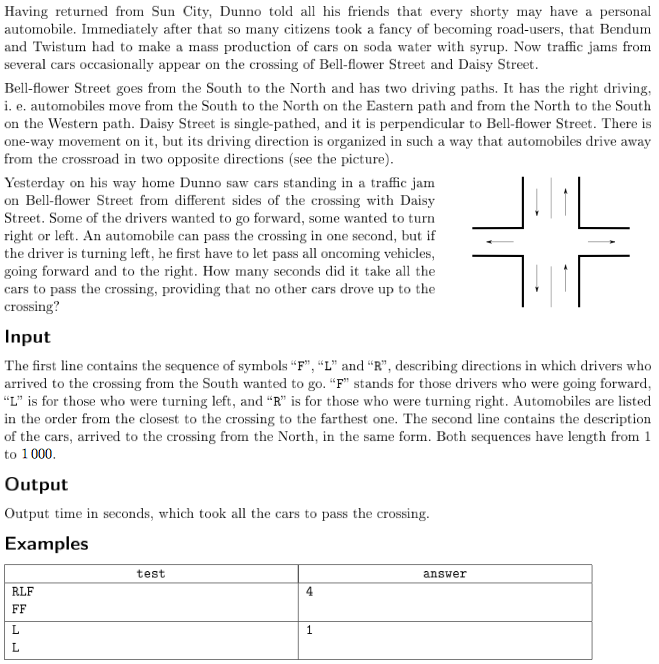
\includegraphics[width=0.9\textwidth]{CT_ACM_EAST/CT_ACM_EAST_I.png}\\ [1cm]
\end{center}
\textbf{{\large Алгоритм}} \\
Считываем водителей с юга, затем с севера. Затем в цикле в порядке заданных приоритетов пропускаем водителей и считаем время. Сложность $O(n)$. \\ 
\\
\newpage
\textbf{{\large Исходный код}}
\begin{lstlisting}[language=C]
#include <iostream>
#include <deque>

using namespace std;

int main() 
{
    deque <char> south;
    deque <char> north;

    char temp;
    int time = 0;
    temp = cin.get();
    while(temp != '\n'){
        south.push_back(temp);
        temp = cin.get();
    }
    temp = cin.get();
    while(temp != '\n'){
        north.push_back(temp);
        temp = cin.get();
    }
    char s, n;
    while(south.size() > 0 && north.size() > 0){
        s = south[0];
        n = north[0];
        time++;
        if(s == 'R' && n == 'L')
            south.pop_front();
        else if(s == 'L' && n == 'R')
            north.pop_front();
         else if(s == 'L' && n == 'F')
            north.pop_front();
         else if(s == 'F' && n == 'L')
            south.pop_front();
         else {
            south.pop_front();
            north.pop_front();
         }
    }
    
    if(south.size() > 0)
        time += south.size();
    if(north.size() > 0)
        time += north.size();

    cout << time << endl;
    return 0;
}
\end{lstlisting}

\newpage
\textbf{{\large Задача L - Donald is a postman}} \\
\begin{center}
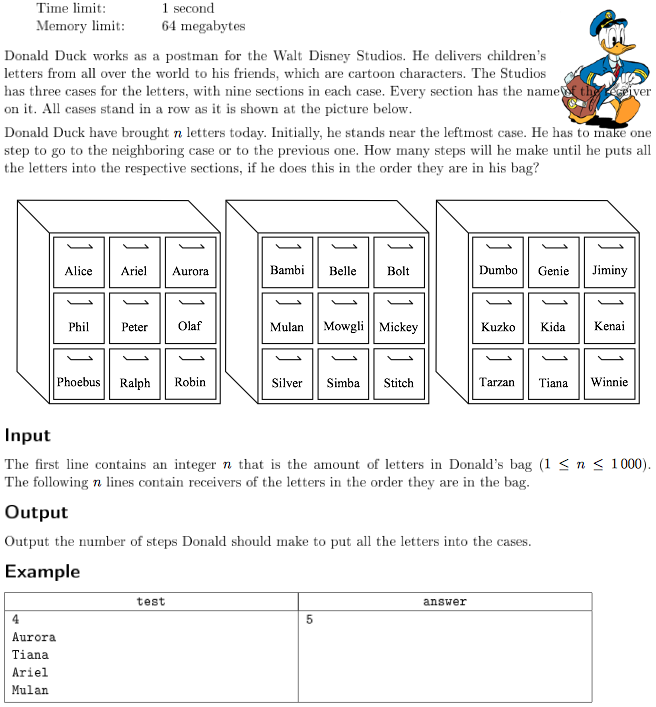
\includegraphics[width=0.9\textwidth]{CT_ACM_EAST/CT_ACM_EAST_L.png}\\ [1cm]
\end{center}
\textbf{{\large Алгоритм}} \\
Задача на реализацию. Нужно симулировать перемещение между состояниями в зависимости от первой буквы имени. Сложность $O(n)$.\\ 
\\
\newpage
\textbf{{\large Исходный код}}
\begin{lstlisting}[language=C]
#include <iostream>

using namespace std;

int main() 
{
    int n;
    cin >> n;
    string name;
    int state = 1;
    int answer = 0;
    for (int i = 0; i < n; i++) {
        cin >> name;
        char t = name[0];
        if (state == 1) {
            if (t == 'B' || t == 'M' || t == 'S') {
                answer++;
                state = 2;
            }
            else if (t == 'D' || t == 'J' || t == 'K' || t == 'T' || t == 'W' || t == 'G') {
                answer += 2;
                state = 3;
            }
        }
        else if (state == 2) {
            if (t == 'A' || t == 'P' || t == 'O' || t == 'R') {
                answer++;
                state = 1;
            }
            else if (t == 'D' || t == 'J' || t == 'K' || t == 'T' || t == 'W' || t == 'G') {
                answer++;
                state = 3;
            }
                
        }
        else {
            if (t == 'A' || t == 'P' || t == 'O' || t == 'R') {
                answer += 2;
                state = 1;
            }
            else if (t == 'B' || t == 'M' || t == 'S') {
                answer++;
                state = 2;
            }
        }
    }
    
    cout << answer << endl;
    return 0;
}
\end{lstlisting}

\newpage
\textbf{{\large Результаты}} \\
\begin{center}
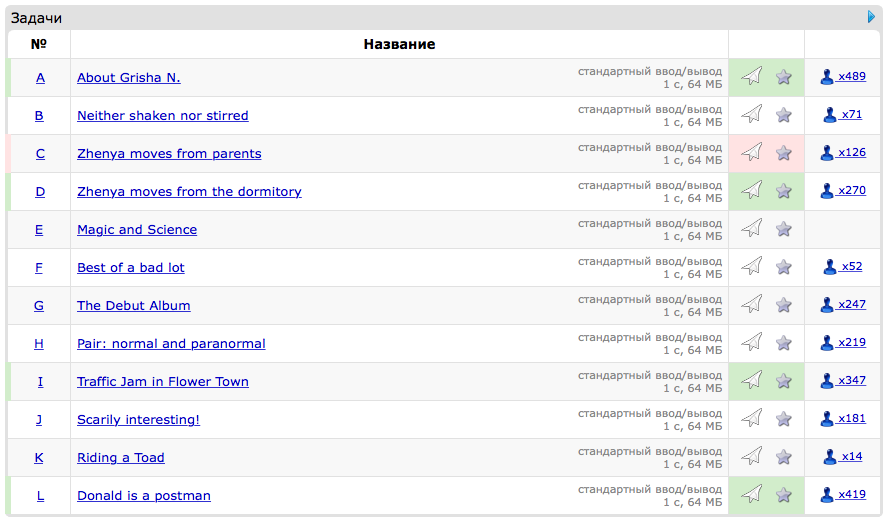
\includegraphics[width=0.95\textwidth]{CT_ACM_EAST/CT_ACM_EAST_result.png}\\ [1cm]
\end{center}



%----------------------------------------------------------------------------------------
%
%	Codeforces ACM Южный четвертьфинал
%
%----------------------------------------------------------------------------------------
\newpage
\subsection{Codeforces ACM-ICPC Южный четвертьфинал}

\textbf{{\large Задача D - Data Center}} \\
\begin{center}
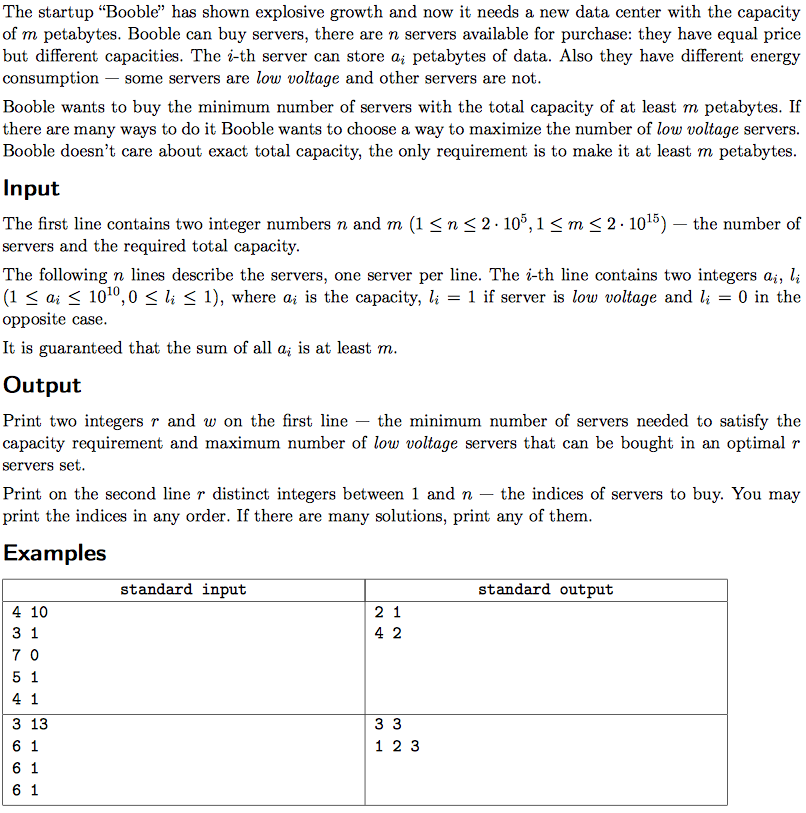
\includegraphics[width=0.9\textwidth]{CT_ACM_WEST/CT_ACM_WEST_D.png}\\ [1cm]
\end{center}
\textbf{{\large Алгоритм}} \\
Сначала отсортируем сервера по объему памяти. Наберем необходимое количество серверов и сравним набранную память с минимальным объемом. Если разница равна $0$, то ответ найден. Иначе будем пытаться поменять сервера с высоким напряжением на сервера с низким напряжением. Сложность $O(n^2)$.\\ 
\\
\newpage
\textbf{{\large Исходный код}}
\begin{lstlisting}[language=C]
#include <iostream>
#include <vector>
#include <algorithm>
#include <fstream>

using namespace std;

typedef struct {
    LL num;
    ULL cap;
    short low;
} server;

bool cmp_low(const server &a, const server &b) {
    return a.low > b.low;
}

bool cmp_cap(const server &a, const server &b) {
    if (a.cap == b.cap) return a.low > b.low;
    return a.cap > b.cap;
}

int main() {
    LL n;
    ULL m;
    cin >> n >> m;
    vector<server> s(n);
    for (LL i = 0; i < n; i++) {
        s[i].num = i + 1;
        cin >> s[i].cap;
        cin >> s[i].low;
    }
    
    sort(s.begin(), s.end(), cmp_cap);
    LL ind = 0;
    ULL curr_cap = 0;
    LL count = 0;

    while (curr_cap < m) {
        curr_cap += s[ind].cap;
        if (s[ind].low) count++;
        ind++;
    }
    
    ULL rem = curr_cap - m;
    
    if (rem == 0) {
        cout << ind << " ";
        cout << count << endl;
        for (LL i = 0; i < ind; i++) {
            cout << s[i].num << " ";
        }
        cout << endl;
        return 0;
    }
    
    for (LL i = ind - 1; i >= 0; i--) {
        if (!s[i].low && rem > 0) {
            bool azaza = false;
            for (LL j = ind; j < n; j++) {
                if (s[j].low && (s[j].cap + rem >= s[i].cap)) {
                    rem -= s[i].cap - s[j].cap;
                    swap(s[i], s[j]);
                    count++;
                    azaza = true;
                    break;
                }
            }
            if (!azaza) break;
        }
        else if (rem == 0) break;
    }
    
    cout << ind << " " << count << endl;
    for (LL i = 0; i < ind; i++) {
        cout << s[i].num << " ";
    }
    cout << endl;;
	return 0;
}
\end{lstlisting}

\newpage
\textbf{{\large Задача I - Sales in GameStore}} \\
\begin{center}
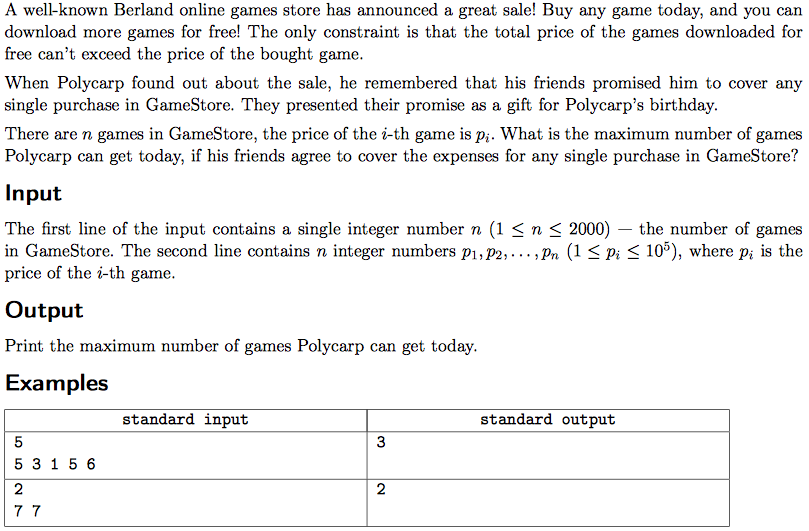
\includegraphics[width=0.9\textwidth]{CT_ACM_WEST/CT_ACM_WEST_I.png}\\ [1cm]
\end{center}
\textbf{{\large Алгоритм}} \\
Отсортируем цены по возрастанию. Затем будем складывать цены по порядку из возрастания и будем считать количество сложений, пока сумма не станет больше максимальной цены. В ответе выведем значение счётчика сложений. Сложность $O(n)$.  \\ 
\\
\newpage
\textbf{{\large Исходный код}}
\begin{lstlisting}[language=C]
#include <iostream>
#include <vector>
#include <algorithm>
using namespace std;
bool compare(const int &a, const int &b)
{
    return a<b;
}
int main(int argc, const char * argv[]) {
    vector<int> p(2001);
    int n;
    cin >> n;
    for(int i=0; i<n; ++i)
        cin >> p[i];
    sort(p.begin(), p.begin()+n);
    int sum = 0;
    int i=0;
    while(i<n-1 && sum+p[i]<=p[n-1])
        sum += p[i++];
    cout << i+1;
    return 0;
}
\end{lstlisting}

\newpage
\textbf{{\large Задача M - Variable Shadowing}} \\
\begin{center}
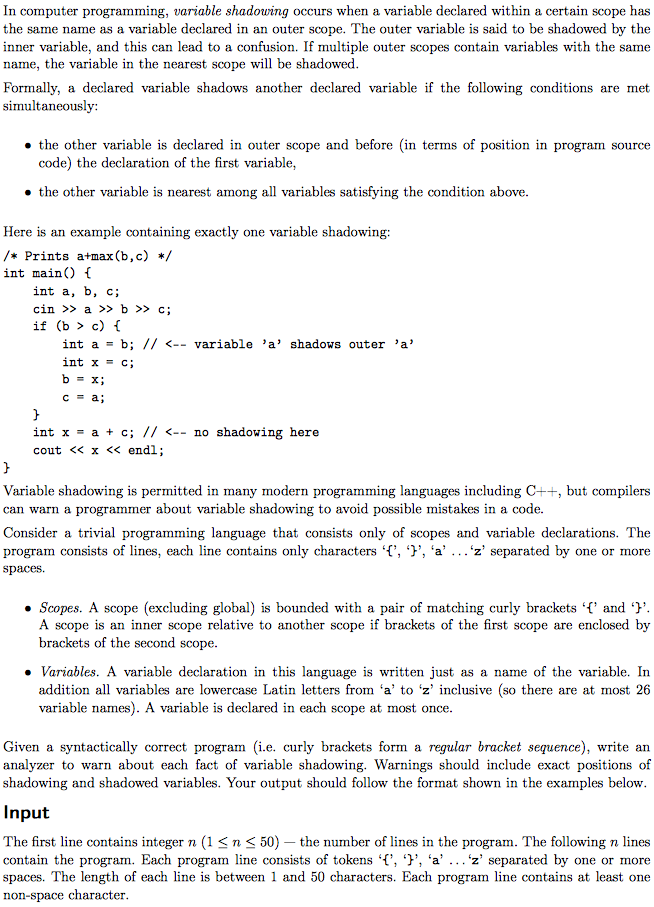
\includegraphics[width=0.9\textwidth]{CT_ACM_WEST/CT_ACM_WEST_M1.png}\\ [1cm]
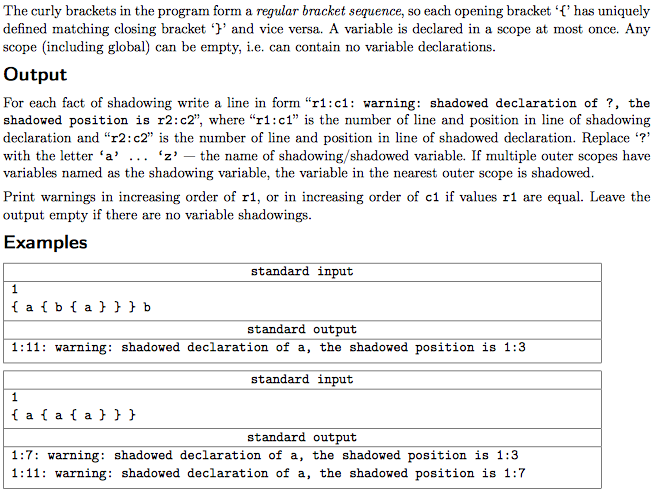
\includegraphics[width=0.9\textwidth]{CT_ACM_WEST/CT_ACM_WEST_M2.png}\\ [1cm]
\end{center}
\textbf{{\large Алгоритм}} \\
Задачу можно решить с помощью стека и вектора стеков. Предупреждение нужно выводить когда новая переменная пытается попасть в стек, который не пуст, это значит уже была объявлена переменная с таким же именем. Когда появляется закрывающая скобка убираем все до открывающей. \\ 
\\
\newpage
\textbf{{\large Исходный код}}
\begin{lstlisting}[language=C]
#include <iostream>
#include <vector>
#include <algorithm>
using namespace std;
typedef struct {
    char ch;
    int line;
    int sym;
} var;
int main() {
    int f,n;
    cin >> n;
    vector <stack <var> > all_alph(26);
    stack <var> curr;
    char temp;
    int symbol = 0;
    var to_put;
    temp = cin.get();
    for (int i = 1; i <= n; i++){
        temp = cin.get();
        symbol = 1;
        while(temp != '\n') {
            if(temp == '}') {
                to_put = curr.top();
                curr.pop();
                while (to_put.ch != '{') {
                    all_alph[to_put.ch - 97].pop();
                    to_put = curr.top();
                    curr.pop();
                }
            }
            else if(temp == '{') {
                to_put.ch = temp;
                to_put.sym = symbol;
                to_put.line = i;
                curr.push(to_put);
            }
            else if (temp != ' '){
                to_put.sym = symbol;
                to_put.line = i;
                to_put.ch = temp;
                curr.push(to_put);
                if(all_alph[temp - 97].size() != 0)
                    cout << to_put.line << ":" << to_put.sym 
                    << ": warning: shadowed declaration of "<< to_put.ch 
                    << ", the shadowed position is " << all_alph[temp - 97].top().line
                    << ":" << all_alph[temp - 97].top().sym << endl;
                all_alph[temp - 97].push(to_put);
            }
            
            temp = cin.get();
            symbol++;
        }
    }
    return 0;
}
\end{lstlisting}

\newpage
\textbf{{\large Результаты}} \\
\begin{center}
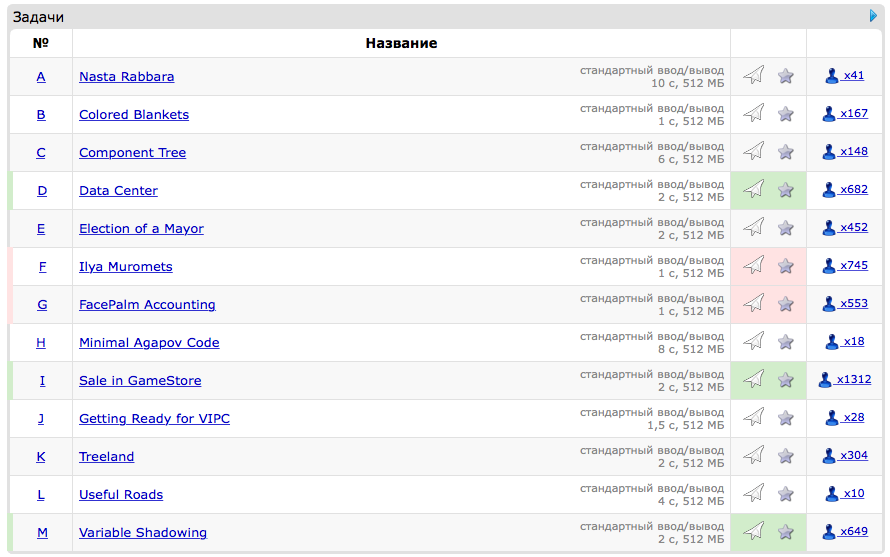
\includegraphics[width=0.95\textwidth]{CT_ACM_WEST/CT_ACM_WEST_result.png}\\ [1cm]
\end{center}



%----------------------------------------------------------------------------------------
%
%	ACM 1/4 Final
%
%----------------------------------------------------------------------------------------
\newpage
\subsection{ACM-ICPC Московский четвертьфинал}

Так как соревнование проводилось в МГУ, то турнирная таблица с результатами и исходные коды программ не доступны. \\



%----------------------------------------------------------------------------------------
%
%	Codeforces Training S02E07
%
%----------------------------------------------------------------------------------------
\newpage
\subsection{Codeforces Training S02E07}

\textbf{{\large Задача C - Will It Stop?}} \\
\begin{center}
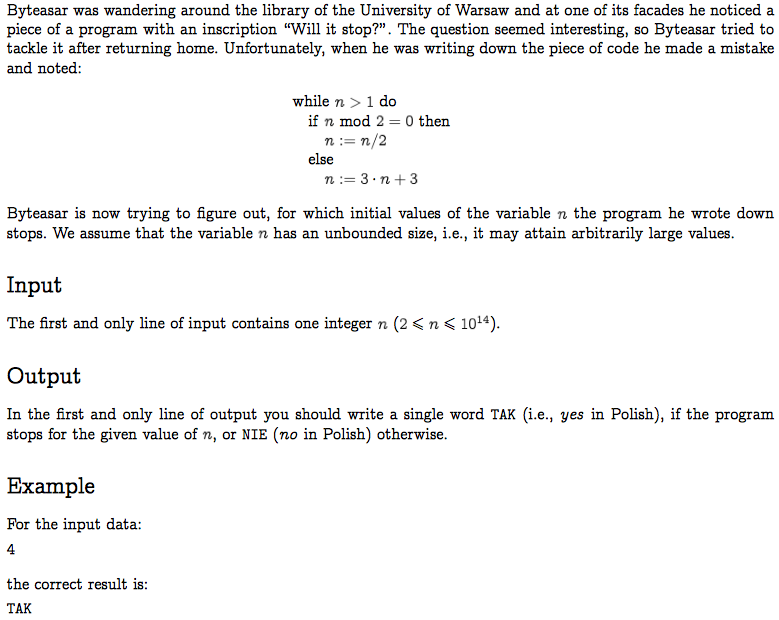
\includegraphics[width=0.9\textwidth]{CT_S02E07/CT_S02E07_C.png}\\ [1cm]
\end{center}
\textbf{{\large Алгоритм}} \\
Делим число n на 2 до тех пор пока оно не перестанет делиться на 2. Если получившееся число равно единице, то выводим $TAK$, если нет, то $NIE$. \\ 

\textbf{{\large Исходный код}}
\begin{lstlisting}[language=C]
#include <iostream>
using namespace std;
int main()
{
    unsigned long long a;
    cin >> a;
    while(!(a%2))a/=2;
    if(a==1)
        cout << "TAK";
    else
        cout << "NIE";
    return 0;
}
\end{lstlisting}

\newpage
\textbf{{\large Задача H - Afternoon Tea}} \\
\begin{center}
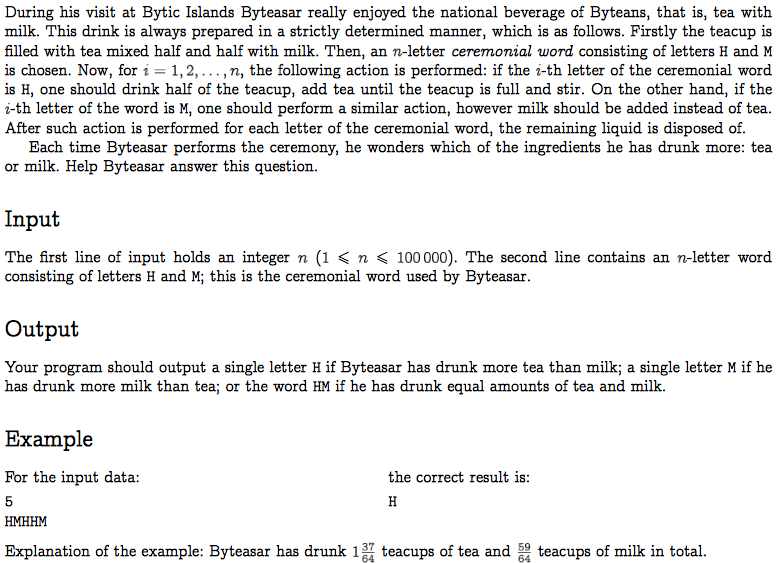
\includegraphics[width=0.9\textwidth]{CT_S02E07/CT_S02E07_H.png}\\ [1cm]
\end{center}
\textbf{{\large Алгоритм}} \\
Создадим две переменные одну для чая, другую для молока и будем последовательно, для каждой буквы, добавлять к ним значение зависящее от позиции текущей буквы, и посчитанное по выведенной формуле. Сложность O(n). \\ 

\textbf{{\large Исходный код}}
\begin{lstlisting}[language=C]
#include <iostream>
#include <cmath>
using namespace std;
int main()
{
    int n;
    cin >> n;
    if(n==1)
    {
        cout << "HM";
        return 0;
    }
    cin.get();
    char c;
    long double hDrunked = 0, mDrunked = 0;
    hDrunked = mDrunked = (1-pow(0.5, n))*0.5;
    for(int i=0; i<n-1; ++i)
    {
        c=cin.get();
        if(c=='H')
            hDrunked += (1-pow(0.5, n-i-1))*0.5;
        else
            mDrunked += (1-pow(0.5, n-i-1))*0.5;
    }
    if(hDrunked>mDrunked)
        cout << "H";
    else if(hDrunked<mDrunked)
        cout << "M";
    return 0;
}
\end{lstlisting}

\textbf{{\large Результаты}} \\
\begin{center}
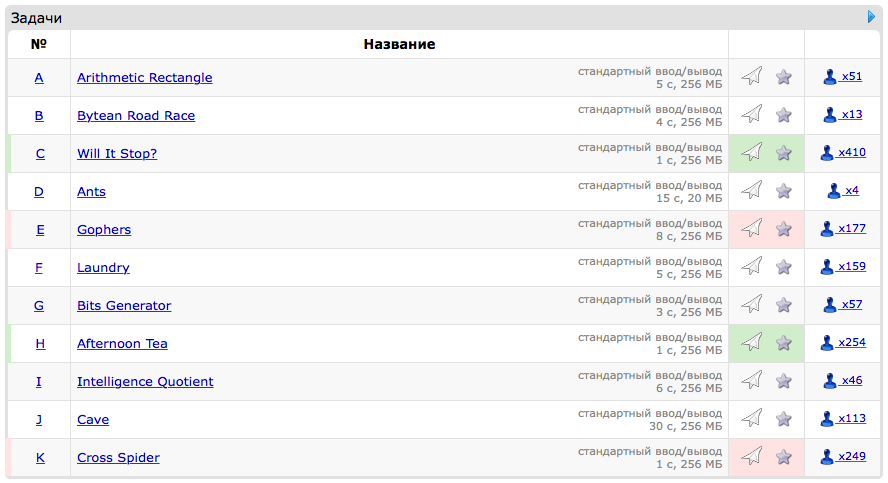
\includegraphics[width=0.95\textwidth]{CT_S02E07/CT_S02E07_result.png}\\ [1cm]
\end{center}



%----------------------------------------------------------------------------------------
%
%	Codeforces Crypto Cup
%
%----------------------------------------------------------------------------------------
\newpage
\subsection{Codeforces Crypto Cup 1.0}

\textbf{{\large Задача B - :-P}} \\
\begin{center}
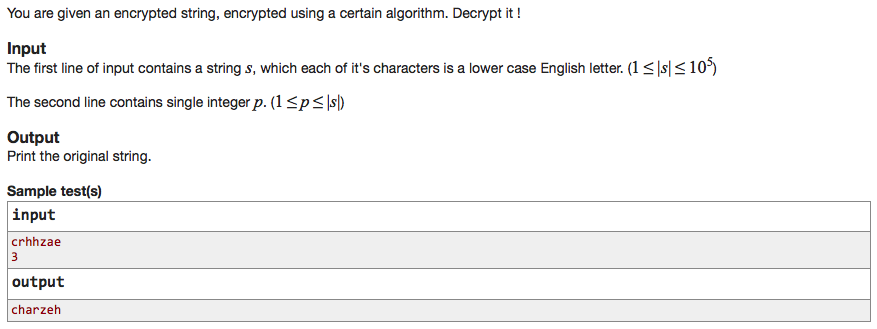
\includegraphics[width=0.9\textwidth]{CT_Crypto/CT_Crypto_B.png}\\ [1cm]
\end{center}

\textbf{{\large Исходный код}}
\begin{lstlisting}[language=C]
#include <iostream>
#include <cmath>
#include <vector>
using namespace std;
int main(int argc, const char * argv[]) {
    char str[100001];
    long p, len;
    while((str[len]=cin.get())!='\n') ++len;
    str[len] = '\0';
    cin >> p;
    vector< vector <char> > v(p);
    long vSize = len/p, r = len%p;
    for(long i=r; i<p; ++i) {
        v[i].resize(vSize);
    }
    for(long i=0; i<r; ++i) {
        v[i].resize(vSize+1);
    }
    for(long i=0, k=0; i<p; ++i) {
        for(long j=0; j<v[i].size(); ++j, ++k) {
            v[i][j] = str[k];
        }
    }
    for(long i=0; i<len; ++i) {
        cout.put(v[i%p][i/p]);
    }
    return 0;
}
\end{lstlisting}

\newpage
\textbf{{\large Задача C - Pgkpxumgs}} \\
\begin{center}
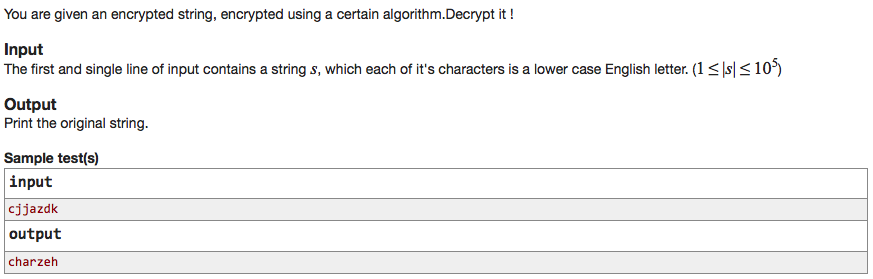
\includegraphics[width=0.9\textwidth]{CT_Crypto/CT_Crypto_C.png}\\ [1cm]
\end{center}

\textbf{{\large Исходный код}}
\begin{lstlisting}[language=C]
#include <iostream>
#include <cstdio>
using namespace std;
int main() {
	char cur, prev;
	cout.put(prev = cin.get());
	while ((cur = cin.get()) != '\n') {
		if ((int)(cur - prev) < 0) cout << (char)(cur - prev + '{');
		else cout << (char)(cur - prev + 'a');
		prev = cur;
 	}
	return 0;
}
\end{lstlisting}

\newpage
\textbf{{\large Задача H - Peace of AmericaReunion}} \\
\begin{center}
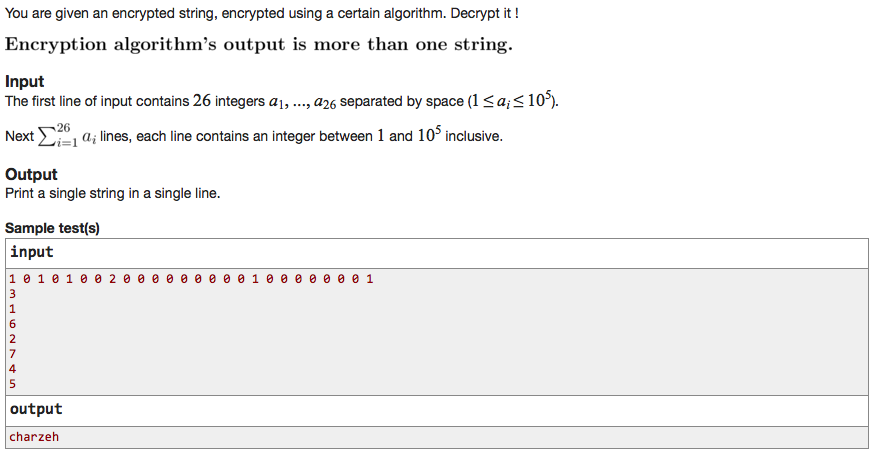
\includegraphics[width=0.9\textwidth]{CT_Crypto/CT_Crypto_H.png}\\ [1cm]
\end{center}

\textbf{{\large Исходный код}}
\begin{lstlisting}[language=C]
#include <iostream>
using namespace std;
int main() {
	vector<long> v(26);
	long length = 0;
	for (int i = 0; i < 26; i++) {
		cin >> v[i];
		length += v[i];
	}
	vector<char> answer(length);
	long pos;
	int nextSymb = -1;
	for (int i = 0; i < 26; i++) {
		if (v[i]) {
			nextSymb = i;
			break;
		}
	}
	for (long i = 0; i < length; i++) {
		cin >> pos;
		if (!v[nextSymb]) {
			for (int i = nextSymb; i < 26; i++) {
				if (v[i]) {
					nextSymb = i;
					break;
				}
			}
		}
		answer[--pos] = (char)(nextSymb + 'a');
		v[nextSymb]--;
	}
	for (auto n : answer) cout << n;
	return 0;
}
\end{lstlisting}

\newpage
\textbf{{\large Задача I - Peace of AmericanPie}} \\
\begin{center}
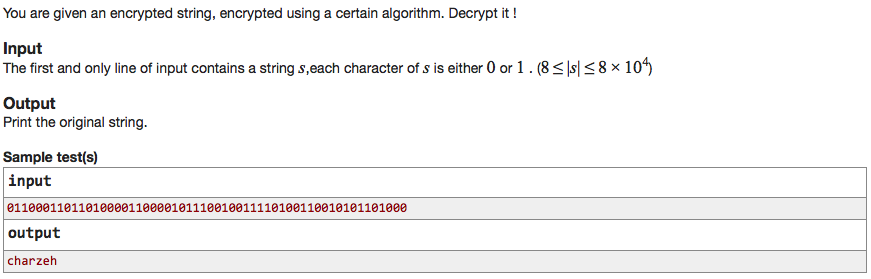
\includegraphics[width=0.9\textwidth]{CT_Crypto/CT_Crypto_I.png}\\ [1cm]
\end{center} 

\textbf{{\large Исходный код}}
\begin{lstlisting}[language=C]
#include <iostream>
using namespace std;
int main() {
	int byte = 0;
	int spow = 256;
	int collected = 0;
	char currentBit;
	while ((currentBit = cin.get()) != '\n') {
		cin.unget();
		while (collected < 8) {
			currentBit = cin.get();
			byte += (currentBit - '0') * spow;
			spow /= 2;
			collected++;
		}
		cout << (char)(byte / 2);
		byte = 0;
		spow = 256;
		collected = 0;
	}
	return 0;
}
\end{lstlisting}

\newpage
\textbf{{\large Задача J - Common}} \\
\begin{center}
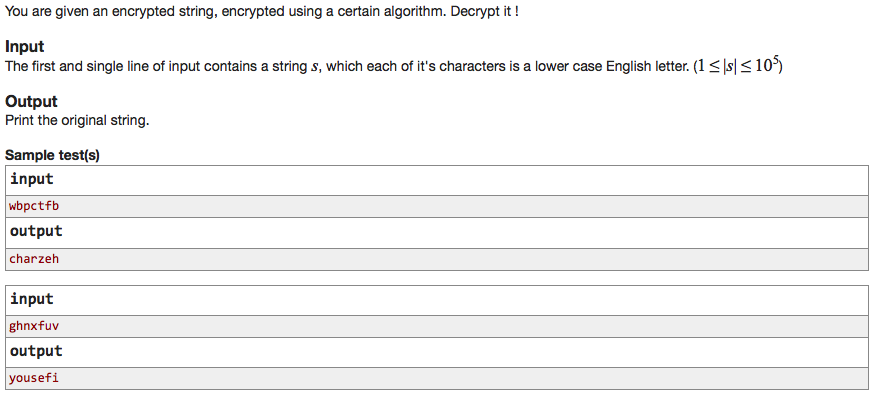
\includegraphics[width=0.9\textwidth]{CT_Crypto/CT_Crypto_J.png}\\ [1cm]
\end{center}

\textbf{{\large Исходный код}}
\begin{lstlisting}[language=C]
#include <iostream>
using namespace std;
int main() {
	char t;
	while ((t = cin.get()) != '\n') {
		switch (t) {
			case 'a':
				cout << "n";
				break;
			case 'b':
				cout << "h";
				break;
			case 'c':
				cout << "r";
				break;
			case 'd':
				cout << "x";
				break;
			case 'e':
				cout << "k";
				break;
			case 'f':
				cout << "e";
				break;
			case 'g':
				cout << "y";
				break;
			case 'h':
				cout << "o";
				break;
			case 'i':
				cout << "q"; 
				break;
			case 'j':
				cout << "m";
				break;
			case 'k':
				cout << "j";
				break;
			case 'l':
				cout << "b";
				break;
			case 'm':
				cout << "d";
				break;
			case 'n':
				cout << "u";
				break;
			case 'o':
				cout << "v";
				break;
			case 'p':
				cout << "a";
				break;
			case 'q':
				cout << "p";
				break;
			case 'r':
				cout << "w";
				break;
			case 's':
				cout << "g";
				break;
			case 't':
				cout << "z";
				break;
			case 'u':
				cout << "f";
				break;
			case 'v':
				cout << "i";
				break;
			case 'w':
				cout << "c";
				break;
			case 'x':
				cout << "s";
				break;
			case 'y':
				cout << "t";
				break;
			case 'z':
				cout << "l";
				break;
		}
	}
	return 0;
}
\end{lstlisting}

\newpage
\textbf{{\large Задача M - oPlus}} \\
\begin{center}
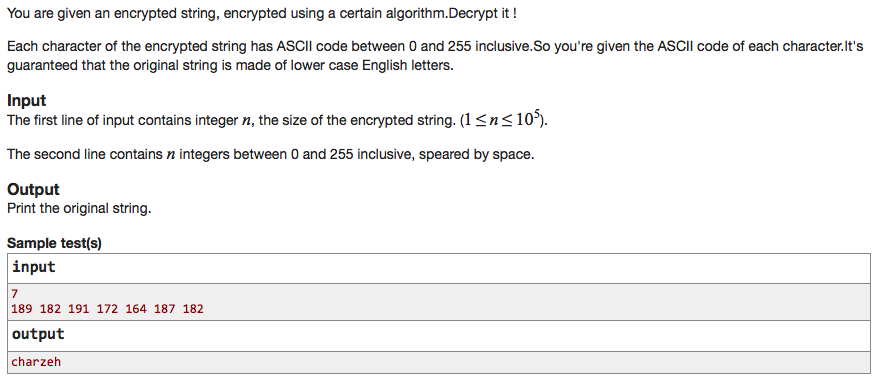
\includegraphics[width=0.9\textwidth]{CT_Crypto/CT_Crypto_M.png}\\ [1cm]
\end{center}

\textbf{{\large Исходный код}}
\begin{lstlisting}[language=C]
#include <iostream>
using namespace std;
int main() {
	long n;
	int curr, sum;
	cin >> n;
	for (long i = 0; i < n; i++) {
		cin >> curr;
		if (curr % 2) sum = 400;
		else sum = 398;
		cout << (char)(sum - curr - 112);
	}
	return 0;
}
\end{lstlisting}

\newpage
\textbf{{\large Задача N - tirnaoeumPt}} \\
\begin{center}
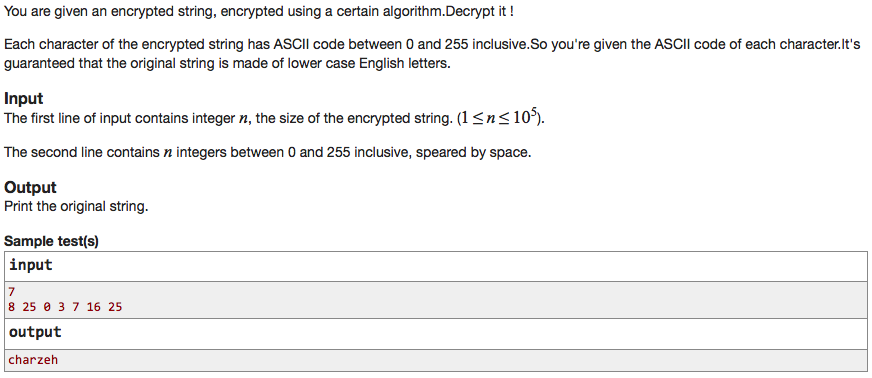
\includegraphics[width=0.9\textwidth]{CT_Crypto/CT_Crypto_N.png}\\ [1cm]
\end{center}

\textbf{{\large Исходный код}}
\begin{lstlisting}[language=C]
#include <iostream>
using namespace std;

int main()
{
    int m[] = {0, 1, 16, 17, 8, 9, 24, 25, 2, 3, 18, 19, 10, 11, 22, 23, 4,  5,  20, 21, 12, 13, 22, 23, 6,  7,  22, 23, 14, 15};
    int n, d;
    cin >> n;
    for(int i=0; i<n; ++i)
    {
        cin >> d;
        cout.put(m[d]+'a');
    }
    return 0;
}
\end{lstlisting}

\newpage
\textbf{{\large Задача Q - Peace of bzjd}} \\
\begin{center}
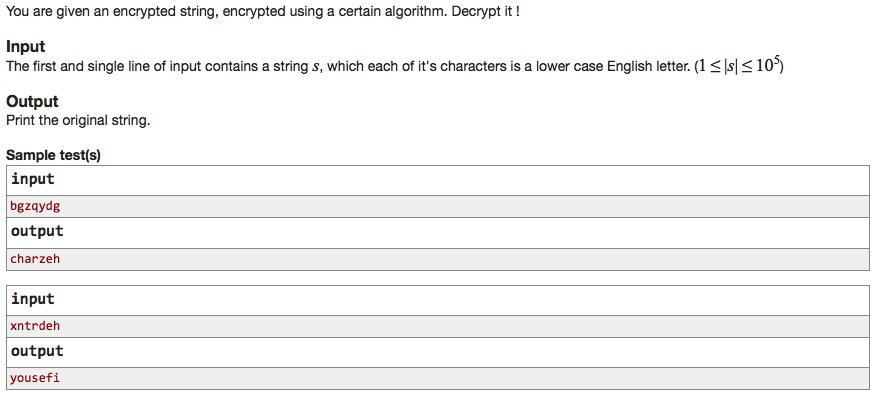
\includegraphics[width=0.9\textwidth]{CT_Crypto/CT_Crypto_Q.png}\\ [1cm]
\end{center}

\textbf{{\large Исходный код}}
\begin{lstlisting}[language=C]
#include <iostream>

using namespace std;

int main()
{
    char temp;
    temp = cin.get();
    while (temp != '\n' && temp != EOF) {
        if (temp == 'z') 
            temp = 'a';
        else temp++;
        cout << temp;
        temp = cin.get();
    }
    return 0;
}
\end{lstlisting}

\newpage
\textbf{{\large Задача R - 6227020800}} \\
\begin{center}
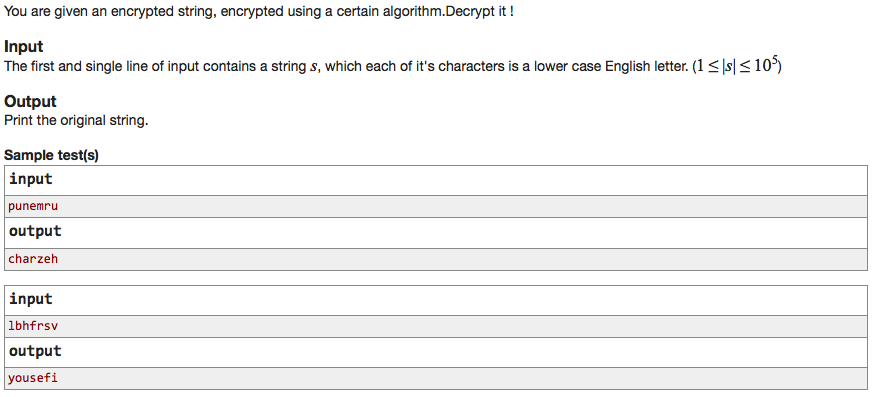
\includegraphics[width=0.9\textwidth]{CT_Crypto/CT_Crypto_R.png}\\ [1cm]
\end{center}

\textbf{{\large Исходный код}}
\begin{lstlisting}[language=C]
#include <iostream>
#include <algorithm>
#include <deque>
#include <cstdio>
using namespace std;
void p(string s) {
	cout << s << endl;
}
int gcd(int a, int b){
    if (b == 0)
        return a;
    return gcd(b, a%b);
}
int main() {
	char t;
	while ((t = cin.get()) != '\n') {
		t -= 13;
		if (t < 'a') {
			cout << (char)('z' - ('a' - t) + 1);
		}
		else {
			cout << t;
		}
	}
	return 0;
}
\end{lstlisting}

\newpage
\textbf{{\large Результаты}} \\
\begin{center}
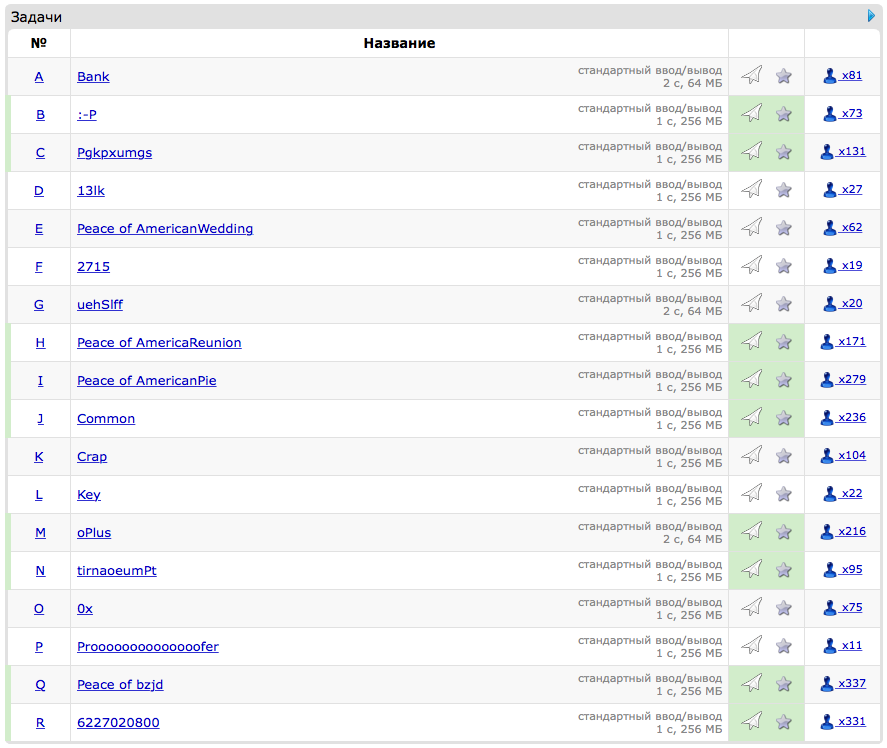
\includegraphics[width=0.95\textwidth]{CT_Crypto/CT_Crypto_result.png}\\ [1cm]
\end{center}



%----------------------------------------------------------------------------------------
%
%	OpenCup GP of Siberia
%
%----------------------------------------------------------------------------------------
\newpage
\subsection{OpenCup GrandPrix of Siberia}

\textbf{{\large Задача 12 - Construction of Chand Baori}} \\
\begin{center}
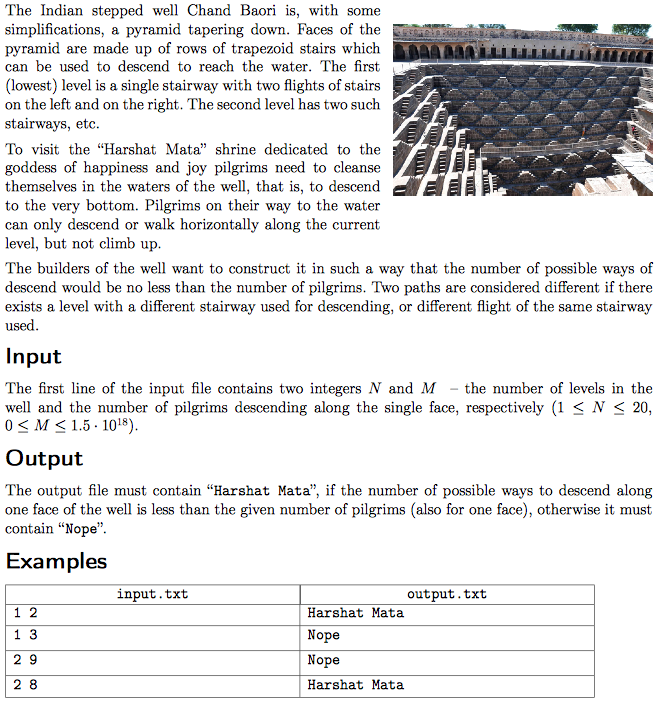
\includegraphics[width=0.9\textwidth]{OC_Siberia/OC_Siberia_12.png}\\ [1cm]
\end{center}
\newpage

\textbf{{\large Алгоритм}} \\
Если $n! > m$, то вывести $Harshat Mata$, если нет, то $Nope$. Сложность $O(n)$. \\ 
\\
%\newpage
\textbf{{\large Исходный код}}
\begin{lstlisting}[language=C++]
#include <iostream>
using namespace std;
#define ULL unsigned long long
int main(int argc, const char * argv[]) {
    ULL n, m;
    cin >> n >> m;
    ULL res = 1;
    for(int i=2; i<=n*2; i+=2)
    {
        res *= i;
    }
    if(res<m)
        cout << "Nope";
    else
        cout << "Harshat Mata";
    return 0;
}
\end{lstlisting}
\newpage
\textbf{{\large Задача 13 - Sum}} \\
\begin{center}
\includegraphics[width=0.9\textwidth]{OC_Siberia/OC_Siberia_13.png}\\ [1cm]
\end{center}
\newpage

\textbf{{\large Алгоритм}} \\
Для того, чтобы подсчитать требуемую сумму можно воспользоваться рекуррентной формулой $a_i = (A * a_{i-1}) \; mod \; P$, где $i \in [2; K]$ и $a_{1} = 1$. Сложность $O(K)$. \\ 
\\
%\newpage
\textbf{{\large Исходный код}}
\begin{lstlisting}[language=C++]
#include <iostream>
#include <fstream>
#include <cmath>
#include <vector>
using namespace std;
#define ULL unsigned long long
#define LL long long
int main(int argc, const char * argv[]) {
    ifstream in("input.txt");
    ofstream out("output.txt");
    ULL a, k, p;
    cin >> a >> k >> p;
    ULL sum = 0, prev = 1;
    for(ULL i = 0; i<k; ++i)
    {
        prev = (prev*a)%p;
        sum += prev;
    }
    cout << sum;
    out.close();
    in.close();
    return 0;
}
\end{lstlisting}
\newpage
\textbf{{\large Задача 14 - Coinquerors}} \\
\begin{center}
\includegraphics[width=0.9\textwidth]{OC_Siberia/OC_Siberia_14_1.png}\\ [1cm]
\includegraphics[width=0.9\textwidth]{OC_Siberia/OC_Siberia_14_2.png}\\ [1cm]

\end{center}
\newpage

\textbf{{\large Алгоритм}} \\
Просто подсчитываем количество пересечений у каждой окружности с остальными и находим ту, у которой это количество максимально. Сложность $O(n^2)$.\\ 
\\
%\newpage
\textbf{{\large Исходный код}}
\begin{lstlisting}[language=C++]
#include <iostream>
#include <fstream>
#include <cmath>
#include <vector>
using namespace std;
#define ULL unsigned long long
#define LL long long
#define eps 0.0001
struct player
{
    char name[256];
    LL x, y, r;
};
int main(int argc, const char * argv[]) {
    ifstream in("input.txt");
    ofstream out("output.txt");
    ULL T;
    in >> T;
    double pi81 = M_PI/81, pi2 = M_PI*2;
    for(ULL TT = 0; TT<T; ++TT)
    {
        ULL n;
        in >> n;
        vector<player> pl(n);
        for(int i=0; i<n; ++i)
        {
            in >> pl[i].name >> pl[i].x >> pl[i].y >> pl[i].r;
        }
        ULL maxInd = -1, max = 0, forTie = -1;
        for(int i=0; i<n; ++i)
        {
            ULL count = 0;
            LL rr = pl[i].r*pl[i].r;
            for(int j=0; j<n; ++j)
            {
                for(double pi = 0; pi<=pi2; pi += pi81)
                {
                    double x = (pl[j].r-eps)*cos(pi);
                    double y = (pl[j].r-eps)*sin(pi);
                    if((pl[j].x-pl[i].x+x)*(pl[j].x-pl[i].x+x)+(pl[j].y-pl[i].y+y)*(pl[j].y-pl[i].y+y)<=rr)
                    {
                        ++count;
                        break;
                    }
                }
            }
            if(count > max)
            {
                max = count;
                maxInd = i;
                forTie = -1;
            }
            else if(count == max)
            {
                max = count;
                forTie = maxInd;
                maxInd = i;
            }
        }
        if(maxInd == -1 || forTie != -1)
            out << "TIE" << '\n';
        else
            out << pl[maxInd].name << '\n';
    }
    out.close();
    in.close();
    return 0;
}
\end{lstlisting}

\textbf{{\large Результаты}} \\
\begin{center}
\includegraphics[width=0.95\textwidth]{OC_Siberia/OC_Siberia_result.png}\\ [1cm]
\end{center}




%----------------------------------------------------------------------------------------
%
%	Codeforces Training S02E08
%
%----------------------------------------------------------------------------------------
\newpage
\subsection{Codeforces Training S02E08}

\textbf{{\large Задача G - Growling Gears}} \\
\begin{center}
\includegraphics[width=0.9\textwidth]{CT_S02E08/CT_S02E08_G1.png}\\ [1cm]
\includegraphics[width=0.9\textwidth]{CT_S02E08/CT_S02E08_G2.png}\\ [1cm]
\end{center}
\textbf{{\large Алгоритм}} \\
В задаче нужно найти передачу с максимальной скоростью вращения. Для этого мы будем применять формулу $(b * b) / (4 * a) + c$ для каждой передачи. Сложность $O(n^2)$.\\ 
\\
%\newpage
\textbf{{\large Исходный код}}
\begin{lstlisting}[language=C]
#include <iostream>
#include <algorithm>

#include <fstream>

using namespace std;

int main() {
    int k;
    cin >> k;
    int n, a, b, c;
    double max_T = -1000000;
    int max_T_num;
    double temp;

    for(int i = 0; i < k; i++) {
        cin >> n;
        for(int j = 1; j <= n; j++) {
            cin >> a >> b >> c;
            temp = (b * b) / (4 * a) + c;
            if(temp > max_T) {
                max_T = temp;
                max_T_num = j;
            }
        }
        cout << max_T_num << endl;
        max_T = -1000000;
    }
	int q;
	cin >> q;
    return 0;
}
\end{lstlisting}


\newpage
\textbf{{\large Задача J - Jury Jeopardy}} \\
\begin{center}
\includegraphics[width=0.9\textwidth]{CT_S02E08/CT_S02E08_J1.png}\\ [1cm]
\includegraphics[width=0.9\textwidth]{CT_S02E08/CT_S02E08_J2.png}\\ [1cm]
\end{center}
\textbf{{\large Алгоритм}} \\
Создаём матрицу, изначально заполненную решётками. Воспроизводим путь робота согласно входным символам и отмечаем путь точками, в процессе запоминая максимальную и минимальную координаты. Используя найденные граничные координаты, вычисляем размер поля и выводим само поле. Сложность $O(n)$.
\newpage
\textbf{{\large Исходный код}} \\
\begin{lstlisting}[language=C]
#include <iostream>
using namespace std;
int main(int argc, const char * argv[]) {
    long T;
    cin >> T;
    cout << T << '\n';
    char map[201][201];
    cin.get();
    while(T--)
    {
        for(long i=0; i<201; ++i)
            for(long j=0; j<201; ++j)
                map[i][j] = '#';
        char c;
        long x, y, minX, minY, maxX, maxY;
        maxX = maxY = minX = minY = x = y = 100;
        int dir = 0;
        while((c=cin.get())!='\n')
        {
            switch(dir)
            {
                case 0:
                    if(c=='R')
                        dir = 3;
                    else if(c=='L')
                        dir = 1;
                    else if(c=='B')
                        dir = 2;
                    break;
                case 1:
                    if(c=='R')
                        dir = 0;
                    else if(c=='L')
                        dir = 2;
                    else if(c=='B')
                        dir = 3;
                    break;
                case 2:
                    if(c=='R')
                        dir = 1;
                    else if(c=='L')
                        dir = 3;
                    else if(c=='B')
                        dir = 0;
                    break;
                case 3:
                    if(c=='R')
                        dir = 2;
                    else if(c=='L')
                        dir = 0;
                    else if(c=='B')
                        dir = 1;
                    break;
            }
            switch(dir)
            {
                case 0:
                    ++x;
                    if(x>maxX)
                        maxX = x;
                    break;
                case 1:
                    --y;
                    if(y<minY)
                        minY = y;
                    break;
                case 2:
                    --x;
                    if(x<minX)
                        minX = x;
                    break;
                case 3:
                    ++y;
                    if(y>maxY)
                        maxY = y;
                    break;
            }
            map[x][y] = '.';
        }
        cout << maxY-minY+3 << ' ' << maxX-minX+2 << '\n';
        for(long i = minY-1; i<=maxY+1; ++i)
        {
            for(long j = minX; j<=maxX+1; ++j)
                cout.put(map[j][i]);
            cout.put('\n');
        }
    }
    return 0;
}
\end{lstlisting}

\textbf{{\large Результаты}} \\
\begin{center}
\includegraphics[width=0.95\textwidth]{CT_S02E05/CT_S02E05_result.png}\\ [1cm]
\end{center}



%----------------------------------------------------------------------------------------
%
%	Codeforces Training S02E09
%
%----------------------------------------------------------------------------------------
\newpage
\subsection{Codeforces Training S02E09}

\textbf{{\large Задача G - Graveyard}} \\
\begin{center}
\includegraphics[width=0.9\textwidth]{CT_S02E09/CT_S02E09_G.png}\\ [1cm]
\end{center}
\textbf{{\large Алгоритм}} \\
Для того, чтобы решить эту задачу, нужно представить окружность в виде отрезка с длиной $10000$. Разобьём отрезок сначала на $n$ частей и запишем точки в вектор $a$, затем разобьём отрезок на $n+m$ частей и запишем точки в вектор $b$. Найдём пару ближайших точек из векторов $a$ и $b$, расстояние между ними и будет ответом. Сложность $O(n^2+nm)$. \\ 
\\
%\newpage
\textbf{{\large Исходный код}}
\begin{lstlisting}[language=C]
#include <iostream>
#include <vector>
#include <string>
#include <algorithm>
#include <queue>
#include <climits>
#include <cctype>
#include <cmath>
#include <fstream>
#include <iomanip>
#define ll long long
#define ull unsigned long long
using namespace std;
int main()
{
    ifstream in("graveyard.in");
    ofstream out("graveyard.out");
    ll n, m;
    in >> n >> m;
    ll nm = n+m;
    vector<double> a(n);
    vector<double> b(nm);
    double s = 0;
    for(ll i=0; i<n; ++i)
    {
        a[i] = s;
        s += 10000.0/n;
    }
    s = 0;
    for(ll i=0; i<nm; ++i)
    {
        b[i] = s;
        s += 10000.0/nm;
    }
    vector<bool> u(nm, 0);
    vector<double> r(n);
    double res = 0;
    for(ll i=0; i<n; ++i)
    {
        double min = 200000.0;
        for(ll j=0; j<nm; ++j)
        {
            
            if(!u[j] && fabs(a[i]-b[j])<min)
            {
                u[j] = 1;
                min = fabs(a[i]-b[j]);
            }
        }
        res += min;
    }
    out << fixed << setprecision(4) << res;
    in.close();
    out.close();
    return 0;
}
\end{lstlisting}


\newpage
\textbf{{\large Задача J - Java vs C++}} \\
\begin{center}
\includegraphics[width=0.9\textwidth]{CT_S02E09/CT_S02E09_J.png}\\ [1cm]
\end{center}
\textbf{{\large Алгоритм}} \\
Посимвольно считываем и проверяем на признаки $Java$ и $C++$. Если обнаружились оба признака, то выводим ошибку. Если только один, то приводим строку к соответствующему формату. Сложность $O(n)$.
\newpage
\textbf{{\large Исходный код}} \\
\begin{lstlisting}[language=C]
#include <iostream>
#define ll long long
#define ull unsigned long long
#define ERROR {out << "Error!"; return 0;}
using namespace std;
int main()
{
    ifstream in("java_c.in");
    ofstream out("java_c.out");
    char c;
    bool java = 0, cpp = 0, us = 0;
    char str[1000];
    ll n=0;
    while(!in.eof() && (c=in.get())!='\n')
    {
        if(in.eof())
            break;
        if(c=='_')
        {
            if(us || !n)
                ERROR
            cpp = 1;
            us = 1;
        }
        else if(isupper(c))
        {
            if(!n)
                ERROR
            java = 1;
            str[n++] = '_';
            str[n++] = tolower(c);
        }
        else if(us)
            str[n++] = toupper(c);
        else
            str[n++] = c;
        if(c!='_')
            us = 0;
        if(java && cpp)
            ERROR
    }
    str[n] = '\0';
    if(n&&!us)
        out << str;
    else
        out << "Error!";
    in.close();
    out.close();
    return 0;
}
\end{lstlisting}

\newpage
\textbf{{\large Задача K - Kickdown}} \\
\begin{center}
\includegraphics[width=0.9\textwidth]{CT_S02E09/CT_S02E09_K.png}\\ [1cm]
\end{center}
\textbf{{\large Алгоритм}} \\
Для решения этой задачи нужно подвигать шестеренки влево и вправо, проверить совпадение и выбрать ответ с наибольшим совпадением.
\newpage
\textbf{{\large Исходный код}} \\
\begin{lstlisting}[language=C]
#include <iostream>
#include <fstream>

bool checkGears1(string master, string driven, int pos) {
    for (int i = 0; pos < master.length() && i < driven.length(); i++) {
        if (master[pos] == driven[i])
            if (master[pos] == '2')
                return false;
        pos++;
    }
    return true;
}

bool checkGears2(string master, string driven, int pos) {
    for (int i = 0; i < master.length() && pos < driven.length(); i++) {
        if (master[i] == driven[pos])
            if (master[i] == '2')
                return false;
        pos++;
    }
    return true;
}

int main() {
	ifstream in("kickdown.in");
    ofstream out("kickdown.out");
    string master, driven;
    in >> master >> driven;
    if (master.length() < driven.length()) swap(master, driven);
    
    int pos1 = 0;
    while (pos1 < master.length() && !checkGears1(master, driven, pos1)) pos1++;
    
    int pos2 = 0;
    while (pos2 < master.length() && !checkGears2(master, driven, pos2)) pos2++;
    
    int d1 = (int)(driven.length() + pos1 - master.length());
    int diff1 = (d1 >= 0) ? d1 : 0;
    int diff2 = pos2;
    
    if (diff1 < diff2) {
        out << max(master.length(), driven.length() + pos1) << endl;
    }
    else {
        out << master.length() + pos2 << endl;
    }
    
    in.close();
    out.close();
    
    return 0;
}
\end{lstlisting}

\textbf{{\large Результаты}} \\
\begin{center}
\includegraphics[width=0.95\textwidth]{CT_S02E09/CT_S02E09_result.png}\\ [1cm]
\end{center}



%----------------------------------------------------------------------------------------
%
%	Codeforces Олимпиада школьников НН
%
%----------------------------------------------------------------------------------------
\newpage
\subsection{Codeforces Олимпиада школьников Нижегородской обл.}

\textbf{{\large Задача A - Выравнивание вещественных чисел}} \\
\begin{center}
\includegraphics[width=0.9\textwidth]{CT_school_nn/CT_school_nn_A.png}\\ [1cm]
\end{center}
\textbf{{\large Алгоритм}} \\
Находим число с максимальным количеством цифр перед точкой. Добавляем к остальным числам спереди решётки чтобы перед точкой количество символов стало равно максимальному. Сложность $O(n)$. \\ 
\\
%\newpage
\textbf{{\large Исходный код}}
\begin{lstlisting}[language=C]
#include <iostream>
#include <cmath>
#define ll long long
#define ull unsigned long long
using namespace std;
int main()
{
    ll n;
    cin >> n;
    char num[1000][2010];
    int logs[1000];
    ll maxLog = 1;
    cin.get();
    for(ll i=0; i<n; ++i)
    {
        ll j=0;
        logs[i] = 0;
        bool pf = 0;
        while((num[i][j]=cin.get())!='\n')
        {
            if(num[i][j] == '.')
                pf = 1;
            if(!pf)
                ++logs[i];
            ++j;
        }
        num[i][j++] = '\0';
        if(logs[i]>maxLog)
            maxLog = logs[i];
    }
    for(ll i=0; i<n; ++i)
    {
        for(ll j=0; j<maxLog-logs[i]; ++j)
            cout.put('#');
        cout << num[i] << '\n';
    }
    return 0;
}
\end{lstlisting}


\newpage
\textbf{{\large Задача F - Фоторамка}} \\
\begin{center}
\includegraphics[width=0.9\textwidth]{CT_school_nn/CT_school_nn_F.png}\\ [1cm]
\end{center}
\textbf{{\large Алгоритм}} \\
В этой задаче можно заметить закономерность и предпосчитать ответ, так как всего может быть 20 различных входных данных. Таким образом, сложность составляет $O(1)$.
\newpage
\textbf{{\large Исходный код}} \\
\begin{lstlisting}[language=C]
#include <iostream>
using namespace std;
int main() {
    long long m[]={0, 0, 0, 24, 120, 360, 840, 1680, 3024, 5040, 7920, 11880, 17160, 24024, 32760, 43680, 57120, 73440, 93024, 116280};
    int n;
    cin >> n;
    cout << m[n-1];
    return 0;
}
\end{lstlisting}

\newpage
\textbf{{\large Задача I - Изи}} \\
\begin{center}
\includegraphics[width=0.9\textwidth]{CT_school_nn/CT_school_nn_I.png}\\ [1cm]
\end{center}
\textbf{{\large Алгоритм}} \\
В задаче просто нужно вывести $n - 1$.
\newpage
\textbf{{\large Исходный код}} \\
\begin{lstlisting}[language=C]
#include <iostream>
#include <vector>
#include <string>
#include <algorithm>
#include <queue>
#include <climits>
#include <cctype>
#include <fstream>
#define ll long long
#define ull unsigned long long
using namespace std;
int main()
{
    ll n;
    cin >> n;
    cout << n-1;
    return 0;
}
\end{lstlisting}

\textbf{{\large Результаты}} \\
\begin{center}
\includegraphics[width=0.95\textwidth]{CT_school_nn/CT_school_nn_result.png}\\ [1cm]
\end{center}



%----------------------------------------------------------------------------------------
%
%	OpenCup GP of Central Europe
%
%----------------------------------------------------------------------------------------
\newpage
\subsection{OpenCup GrandPrix of Central Europe}

\textbf{{\large Задача A - Адокат}} \\
\begin{center}
\includegraphics[width=0.9\textwidth]{OC_Central_Europe/OC_Central_Europe_A.png}\\ [1cm]
\end{center}
\newpage

\textbf{{\large Алгоритм}} \\
Для каждого дня находим встречу с минимальным времение конца и встречу с максимальным временем начала. Если время конца первой встречи меньше времени конца второй, то выведем $TAK$ и номера встреч, если нет, то выведем $NIE$. Сложность $O(n)$. \\ 
\\
%\newpage
\textbf{{\large Исходный код}}
\begin{lstlisting}[language=C++]
#include <iostream>
#include <fstream>
#include <vector>

using namespace std;

int main()
{
    ll n, m;
    ll a, b, d;
    cin >> n >> m;
    vector< pair<ll, ll> > maxA(m, make_pair(-1, -1)), minB(m, make_pair(-1, -1));
    for (ll i=0; i<n; ++i) {
        cin >> a >> b >> d;
        --d;
        if (maxA[d].second == -1 || maxA[d].second < a) {
            maxA[d].second = a;
            maxA[d].first = i;
        }
        if (minB[d].second == -1 || minB[d].second > b) {
            minB[d].second = b;
            minB[d].first = i;
        }
    }
    for (ll i=0; i<m; ++i) {
        if (minB[i].second < maxA[i].second) {
            cout << "TAK " << minB[i].first+1 << ' ' << maxA[i].first+1 << '\n';
        }
        else {
            cout << "NIE\n";
        }
    }
    return 0;
}

\end{lstlisting}

\textbf{{\large Результаты}} \\
\begin{center}
\includegraphics[width=0.95\textwidth]{OC_Central_Europe/OC_Central_Europe_result.png}\\ [1cm]
\end{center}



%----------------------------------------------------------------------------------------
%
%	Codeforces Training S02E10
%
%----------------------------------------------------------------------------------------
\newpage
\subsection{Codeforces Training S02E10}

\textbf{{\large Задача A - Abnormal Coins}} \\
\begin{center}
\includegraphics[width=0.9\textwidth]{CT_S02E10/CT_S02E10_A.png}\\ [1cm]
\end{center}
\textbf{{\large Алгоритм}} \\
Будем считать сумму арифметической прогрессии с начальным членом равным $3$ и разностью $1$ и считать количество итераций в переменную $count$, пока сумма не станет больше числа $n$, тогда ответом будет значение в счётчике $count$. Сложность $O(n)$.  \\ 
\\
%\newpage
\textbf{{\large Исходный код}}
\begin{lstlisting}[language=C]
#include <iostream>
#include <vector>
#include <algorithm
#include <iomanip>
#define ll long long
#define ull unsigned long long
using namespace std;
int main() {
    LL n;
    cin >> n;
    LL count = 0;
    LL sum = 0;
    
    for (LL i = 3; ; i++) {
        sum += i;
        if (sum > n) break;
        count++;
    }
    cout << count << endl;
    return 0;
}
\end{lstlisting}


\newpage
\textbf{{\large Задача B - Fake Coins}} \\
\begin{center}
\includegraphics[width=0.9\textwidth]{CT_S02E10/CT_S02E10_B.png}\\ [1cm]
\end{center}
\textbf{{\large Алгоритм}} \\
Нужно посчитать количество возможных кодов безопасности, которые могу быть сгенерированы. Для этого мы создадим ассоциативный массив и будем последовательно инкрементировать значения по строкам. Ответом будет размер ассоциативного массива. Сложность $O(n^2*log(n))$.
\newpage
\textbf{{\large Исходный код}} \\
\begin{lstlisting}[language=C]
#include <iostream>
#include <map>
#include <vector>
#define ll long long
#define ull unsigned long long
#define ERROR {out << "Error!"; return 0;}
using namespace std;
int main() {
    map<string, int> strings;
    string base, current = "";
    vector<int> spos;
    cin >> base;
    int baseSize = (int)base.size();
    for (int i = 1; i < baseSize; i++) {
        for (int j = i + 1; j <= baseSize; j++) {
            current += base[i - 1];
            current += base[j - 1];
            int cPos = i + j;
            int pPos = j, temp = 0;
            while (cPos <= baseSize) {
                current += base[cPos - 1];
                temp = pPos;
                pPos = cPos;
                cPos += temp;
            }
            strings[current]++;
            current.clear();
        }
    }
    
    cout << strings.size() << endl;
    
    return 0;
}
\end{lstlisting}

\newpage
\textbf{{\large Задача G - Coin Game}} \\
\begin{center}
\includegraphics[width=0.9\textwidth]{CT_S02E10/CT_S02E10_G.png}\\ [1cm]
\end{center}
\textbf{{\large Алгоритм}} \\
Делаем обмены сначала слева направо, потом справа налево, сравниваем в который раз получилось меньше шагов и выводим это количество шагов. Сложность $O(n)$.
\newpage
\textbf{{\large Исходный код}} \\
\begin{lstlisting}[language=C]
#include <iostream>
#include <vector>
#include <map>
#include <cmath>
#include <algorithm>
#include <iomanip>
#include <list>
#include <iterator>
using namespace std;
#define ll long long
#define ull unsigned long long

int main()
{
    char a[25001], b[25001], c;
    int n = 0, first1 = -1, last1 = -1;
    while((c=cin.get())!='\n' && !cin.eof())
    {
        if(first1 == -1 && c == '1')
            first1 = n;
        if(c == '1')
            last1 = n;
        if(cin.eof())
            break;
        a[n] = b[n] = c;
        ++n;
    }
    a[n] = b[n] = '\0';
    ll aCount = 0, bCount = 0;
    for(ll i=0; i<n; ++i)
    {
        if(a[i] == '1')
            continue;
        for(ll j=i+1; j<n; ++j)
        {
            if(a[j] == '1')
            {
                swap(a[i], a[j]);
                aCount += j-i;
                break;
            }
        }
    }
    for(ll i=n-1; i>=0; --i)
    {
        if(b[i] == '1')
            continue;
        for(ll j=i-1; j>=0; --j)
        {
            if(b[j] == '1')
            {
                swap(b[i], b[j]);
                bCount += i-j;
                break;
            }
        }
    }
    if(aCount < bCount)
        cout << aCount;
    else
        cout << bCount;
    return 0;
}
\end{lstlisting}

\textbf{{\large Результаты}} \\
\begin{center}
\includegraphics[width=0.95\textwidth]{CT_S02E10/CT_S02E10_result.png}\\ [1cm]
\end{center}



%----------------------------------------------------------------------------------------
%
%	OpenCup GP of Europe
%
%----------------------------------------------------------------------------------------
\newpage
\subsection{OpenCup GrandPrix of Europe}

\textbf{{\large Задача E - Express As The Sum}} \\
\begin{center}
\includegraphics[width=0.9\textwidth]{OC_Europe/OC_Europe_E.png}\\ [1cm]
\end{center}
\newpage

\textbf{{\large Алгоритм}} \\
Перебираем разложения для всех $N$ пока не найдём нужное, начиная от $2$. с помощью формулы $N/i$ можно сразу найти одно из чисел, входящее в возможное разложение, а затем просто перебрать $i$ вариантов. Сложность $O(n*log(n))$.  \\ 
\\
%\newpage
\textbf{{\large Исходный код}}
\begin{lstlisting}[language=C++]
#include <iostream>
using namespace std;
#define ll long long
#define ull unsigned long long
void answer(ll n, ll l, ll r) {
    cout << n << " = " << l;
    for(ll i=l+1; i<=r; ++i) {
        cout << " + " << i;
    }
    cout.put('\n');
}
int main()
{
    ll T;
    cin >> T;
    while (T--) {
        ll n;
        cin >> n;
        ll t = n;
        bool f = 0;
        while(t!=0) {
            if (t>1 && t&1) {
                f = 1;
                break;
            }
            t >>= 1;
        }
        if(!f) {
            cout << "IMPOSSIBLE\n";
            continue;
        }
        f = 0;
        for (ll i=2; !f && i<100500; ++i) {
            ll sum = 0;
            ll r = n/i;
            ll l = r-i+1;
            if(l<1) {
                l = 1;
                r = l+i-1;
            }
            for(ll j=l; j<=r; ++j) {
                sum += j;
            }
            if(sum == n) {
                answer(n, l, r);
                break;
            }
            for(ll j=r+1; j<r+i; ++j) {
                sum += j-l;
                if(sum == n) {
                    answer(n, l+1, j);
                    f = 1;
                    break;
                }
                ++l;
            }
        }
    }
    return 0;
}
\end{lstlisting}
\newpage
\textbf{{\large Задача F - Factory}} \\
\begin{center}
\includegraphics[width=0.9\textwidth]{OC_Europe/OC_Europe_F.png}\\ [1cm]
\end{center}
\newpage

\textbf{{\large Алгоритм}} \\
Находим пересекающиеся шестерёнки и строим граф их связей. Проходим от первой шестерёнки ко всем остальным с помощью обхода в ширину. Направление вращения чередуется на каждом уровне. Зная радиусы двух смежных шестерёнок и скорость одной из них, легко можно вычислить скорость другой. Сложность $O(n^2)$. \\ 
\\
%\newpage
\textbf{{\large Исходный код}}
\begin{lstlisting}[language=C++]
#include <iostream>
#include <vector>
using namespace std;
#define ll long long
#define ull unsigned long long
#define eps 0.00001
ll min(ll a, ll b){return (a<b?a:b);}
ll max(ll a, ll b){return (a>b?a:b);}

struct Gear {
    int x, y, r;
};

struct GearSpeed {
    ll n, d;
    bool dir;
};
int main()
{
    ll T;
    cin >> T;
    while (T--) {
        ll n;
        cin >> n;

        vector< list<int> > m(n);
        vector<bool> u(n, 0);
        vector<Gear> gears(n);
        for (ll i=0; i<n; ++i) {
            cin >> gears[i].x >> gears[i].y >> gears[i].r;
        }
        for (int i=0; i<n; ++i) {
            for (int j=i+1; j<n; ++j) {
                double x = gears[i].x-gears[j].x;
                double y = gears[i].y-gears[j].y;
                if(sqrt(x*x+y*y)<=gears[i].r+gears[j].r) {
                    m[i].insert(m[i].begin(), j);
                    m[j].insert(m[j].begin(), i);
                }
            }
        }
        vector<GearSpeed> speed(n);
        speed[0].n = 1;
        speed[0].d = 1;
        speed[0].dir = 0;
        queue<int> q;
        q.push(0);
        u[0] = 1;
        while (!q.empty()) {
            int a = q.front();
            q.pop();
            list<int>::iterator it = m[a].begin();
            for (; it!=m[a].end(); ++it) {
                int b = *it;
                if(u[b])
                    continue;
                u[b] = 1;
                speed[b].n = speed[a].n * gears[a].r;
                speed[b].d = speed[a].d * gears[b].r;
                speed[b].dir = !speed[a].dir;
                ll u = speed[b].n;
                ll v = speed[b].d;
                ll temp;
                while (v != 0) {
                    temp = u % v;
                    u = v;
                    v = temp;
                }
                speed[b].n /= u;
                speed[b].d /= u;
                q.push(b);
            }
        }
        for (ll i=0; i<n; ++i) {
            if(!u[i])
                cout << "not moving\n";
            else {
                cout << speed[i].n;
                if(speed[i].d != 1) {
                    cout << '/' << speed[i].d;
                }
                cout.put(' ');
                if(speed[i].dir) {
                    cout << "counterclockwise\n";
                }
                else {
                    cout << "clockwise\n";
                }
            }
        }
    }
    return 0;
}
\end{lstlisting}
\newpage
\textbf{{\large Задача K - Keyboard Troubles}} \\
\begin{center}
\includegraphics[width=0.9\textwidth]{OC_Europe/OC_Europe_K.png}\\ [1cm]
\end{center}
\newpage

\textbf{{\large Алгоритм}} \\
Для этой задачи пришлось заранее предпосчитать массив с правилами перехода между кнопками. Сложность $O(n)$. \\ 
\\
%\newpage
\textbf{{\large Исходный код}}
\begin{lstlisting}[language=C++]
#include <iomanip>
#include <limits>
#include <iostream>
#include <algorithm>

#define LL  long long
#define ULL unsigned long long
#define EPS 1e-11

#define more_speed ios_base::sync_with_stdio(false);

using namespace std;

bool g(int x, int y) {

    if (x == y) return true;

    if (x == 1) {
        return true;
    }
    else if (x == 2) {
        if (y == 3 || y == 5 || y == 6 || y == 8 || y == 9 || y == 0) return true;
    }
    else if (x == 3) {
        if (y == 6 || y == 9) return true;
    }
    else if (x == 4) {
        if (y >= 4 || y == 0) return true;
    }
    else if (x == 5) {
        if (y == 6 || y == 8 || y == 9 || y == 0) return true;
    }
    else if (x == 6) {
        if (y == 9) return true;
    }
    else if (x == 7) {
        if (y >= 7 || y == 0) return true;
    }
    else if (x == 8) {
        if (y == 9 || y == 0) return true;
    }
    return false;
}

int main() {

    more_speed

    int z[] = {0,1,1,1,1,1,1,1,1,1,1,1,1,1,1,1,1,1,1,1,1,0,1,1,0,1,1,0,1,1,0,0,0,1,0,0,1,0,0,1,1,0,0,0,1,1,1,1,1,1,1,0,0,0,0,1,1,0,1,1,0,0,0,0,0,0,1,0,0,1,1,0,0,0,0,0,0,1,1,1,1,0,0,0,0,0,0,0,1,1,0,0,0,0,0,0,0,0,0,1,1,0,0,0,0,0,0,0,0,0,1,1,1,1,1,1,1,1,1,1,1,0,1,1,0,1,1,0,1,1,0,0,0,1,0,0,1,0,0,1,1,0,0,0,1,1,1,1,1,1,1,0,0,0,0,1,1,0,1,1,0,0,0,0,0,0,1,0,0,1,1,0,0,0,0,0,0,1,1,1,1,0,0,0,0,0,0,0,1,1,0,0,0,0,0,0,0,0,0,1,1,0,0,0,0,0,0,0,0,0,0,0,0,0,0,0,0,0,0,0,1,0,1,1,0,1,1,0,1,1,0,0,0,1,0,0,1,0,0,1,0,0,0,0,0,0,0,0,0,0,1,0,0,0,0,1};

    int t;
    cin >> t;

    for (int i = 0; i < t; i++) {
        int n;
        cin >> n;
        if (z[n] == 1) {
            cout << n << endl;
        }
        else {
            int y = n;
            int x = n;
            while (z[x] == 0) {
                x++;
            }
            while (z[y] == 0) {
                y--;
            }
            if (n - y > x - n) {
                cout << x << endl;
            }
            else {
                cout << y << endl;
            }
        }
    }

    return 0;
}
\end{lstlisting}
\newpage
\textbf{{\large Задача O - Allo}} \\
\begin{center}
\includegraphics[width=0.9\textwidth]{OC_Europe/OC_Europe_N.png}\\ [1cm]
\end{center}
\newpage

\textbf{{\large Алгоритм}} \\
Просто отмечаем все цифры, которые встретились в номере в булевском массиве. Потом проходим по этому массиву и проверяем остались ли неотмеченные. Если остались, то выводим их, если нет, то выводим $allo$. Сложность $O(n)$. \\ 
\\
%\newpage
\textbf{{\large Исходный код}}
\begin{lstlisting}[language=C++]
#include <iostream>
#include <vector>
using namespace std;
#define ll long long
#define ull unsigned long long
ll min(ll a, ll b){return (a<b?a:b);}
ll max(ll a, ll b){return (a>b?a:b);}
int main()
{
    ll T;
    cin >> T;
    cin.get();
    while (T--) {
        vector<bool> nums(10, 0);
        char c;
        while((c=cin.get())!='\n' && !cin.eof())
        {
            if(cin.eof())
                break;
            nums[c-'0'] = 1;
        }
        bool f = 0;
        for(ll i=0; i<10; ++i)
        {
            if(!nums[i])
            {
                f = 1;
                cout << i;
            }
        }
        if(!f)
            cout << "allo";
        cout << '\n';
            
    }
    return 0;
}
\end{lstlisting}
\newpage
\textbf{{\large Задача N - C\,-\,-}} \\
\begin{center}
\includegraphics[width=0.9\textwidth]{OC_Europe/OC_Europe_O.png}\\ [1cm]
\end{center}
\newpage

\textbf{{\large Алгоритм}} \\
Задача на реализацию. При объявлении переменной, она добавляется в стек в виде структуры $pair$, в которой первый элемент - значение переменной, а второй - номер области видимости. При выходе из текущей области видимости, все переменный, созданные в ней, удаляются из стека. Сложность $O(n)$. \\ 
\\
%\newpage
\textbf{{\large Исходный код}}
\begin{lstlisting}[language=C++]
#include <iostream>
#include <vector>
using namespace std;
#define ll long long
#define ull unsigned long long
ll min(ll a, ll b){return (a<b?a:b);}
ll max(ll a, ll b){return (a>b?a:b);}
int main()
{
    ll n;
    vector < stack< pair<ll, int> > > vars(26);
    int scope = 0;
    cin >> n;
    char str[20];
    for (int i=0; i<n; ++i) {
        cin >> str;
        if(str[0] == '{') {
            ++scope;
        }
        else if(str[0] == '}') {
            for (int i=0; i<26; ++i) {
                if(!vars[i].empty() && vars[i].top().second == scope) {
                    vars[i].pop();
                }
            }
            --scope;
        }
        else if(str[1] == '=') {
            int c1 = str[0]-'a';
            ll a;
            if(isalpha(str[2])) {
                int c2 = str[2]-'a';
                a = vars[c2].top().first;
                int c1Scope = vars[c1].top().second;
                vars[c1].pop();
                vars[c1].push(make_pair(a, c1Scope));
            }
            else {
                a = 0;
                for (int i=2; str[i]!='\0'; ++i)
                    a = a*10+str[i]-'0';
            }
            int c1Scope = vars[c1].top().second;
            vars[c1].pop();
            vars[c1].push(make_pair(a, c1Scope));
        }
        else if(!strcmp(str, "int")) {
            cin >> str;
            int c;
            c = str[0]-'a';
            vars[c].push(make_pair(-1, scope));
        }
        else if(!strcmp(str, "print")) {
            cin >> str;
            int c = str[0]-'a';
            cout << vars[c].top().first << '\n';
        }
    }
    return 0;
}
\end{lstlisting}

\textbf{{\large Результаты}} \\
\begin{center}
\includegraphics[width=0.95\textwidth]{OC_Europe/OC_Europe_result.png}\\ [1cm]
\end{center}



%----------------------------------------------------------------------------------------
%
%	OpenCup GP of Peterhof
%
%----------------------------------------------------------------------------------------
\newpage
\subsection{OpenCup GrandPrix of Peterhof}

\textbf{{\large Задача H - Некратчайший путь}} \\
\begin{center}
\includegraphics[width=0.9\textwidth]{OC_Peterhof/OC_Peterhof_H1.png}\\ [1cm]
\includegraphics[width=0.9\textwidth]{OC_Peterhof/OC_Peterhof_H2.png}\\ [1cm]
\end{center}
\newpage

\textbf{{\large Алгоритм}} \\
С помощью рекурсии находим все возможные пути и составляем из них вектор. Находим среди них кратчайший и после этого находим путь, который не является кратчайшим, если же не находим, то выводим $-1$. Сложность $O(n^2)$. \\ 
\\
%\newpage
\textbf{{\large Исходный код}}
\begin{lstlisting}[language=C++]
#include <iostream>
#include <vector>
#include <map>
using namespace std;
#define ll long long
#define ull unsigned long long
#define eps 0.00001
ll min(ll a, ll b){return (a<b?a:b);}
ll max(ll a, ll b){return (a>b?a:b);}

vector < vector<char> > paths;
vector<char> path;
size_t __min;

void foo(char map[4][4], int x, int y) {
    if (x == 3 && y == 3) {
        if (path.size() < __min) {
            __min = path.size();
        }
        paths.push_back(path);
    }
    if (x<3 && map[y][x+1] == '.') {
        path.push_back('R');
        map[y][x] = 'X';
        foo(map, x+1, y);
        map[y][x] = '.';
        path.pop_back();
    }
    if (x>0 && map[y][x-1] == '.') {
        path.push_back('L');
        map[y][x] = 'X';
        foo(map, x-1, y);
        map[y][x] = '.';
        path.pop_back();
    }
    map[y][x] = '.';
    if (y<3 && map[y+1][x] == '.') {
        path.push_back('D');
        map[y][x] = 'X';
        foo(map, x, y+1);
        map[y][x] = '.';
        path.pop_back();
    }
    map[y][x] = '.';
    if (y>0 && map[y-1][x] == '.') {
        path.push_back('U');
        map[y][x] = 'X';
        foo(map, x, y-1);
        map[y][x] = '.';
        path.pop_back();
    }
}

int main()
{
    char map[4][4];
    bool e = 1;
    while (e) {
        for (int i=0; i<4; ++i) {
            for (int j=0; j<4; ++j) {
                map[i][j] = cin.get();
            }
            cin.get();
        }
        __min = 100500;
        foo(map, 0, 0);
        bool f = 0;
        for (int i=0; i<paths.size(); ++i) {
            if (paths[i].size() != __min) {
                for (int j=0; j<paths[i].size(); ++j) {
                    cout.put(paths[i][j]);
                }
                f = 1;
                break;
            }
        }
        if (!f) {
            cout << -1;
        }
        cout.put('\n');
        for (int i=0; i<5; ++i) {
            cin.get();
            if (cin.eof()) {
                e = 0;
                break;
            }
        }
        paths.clear();
        path.clear();
    }
    return 0;
}
\end{lstlisting}

\textbf{{\large Результаты}} \\
\begin{center}
\includegraphics[width=0.95\textwidth]{OC_Peterhof/OC_Peterhof_result.png}\\ [1cm]
\end{center}



%----------------------------------------------------------------------------------------
%
%	OpenCup GP of Japan
%
%----------------------------------------------------------------------------------------
\newpage
\subsection{OpenCup GrandPrix of Japan}

\textbf{{\large Задача K - Beads}} \\
\begin{center}
\includegraphics[width=0.9\textwidth]{OC_Japan/OC_Japan_K.png}\\ [1cm]
\end{center}
\newpage

\textbf{{\large Алгоритм}} \\
Для того чтобы решить задачу, нужно найти минимальный циклический сдвиг, для этого мы применим алгоритм Дюваля. Сложность $O(n)$. \\ 
\\
%\newpage
\textbf{{\large Исходный код}}
\begin{lstlisting}[language=C++]
#include <iostream>

using namespace std;

long min_cyclic_shift (string s) {
    s += s;
    long n = (long) s.length();
    long i = 0, ans = 0;
    while (i < n/2) {
        ans = i;
        long j = i + 1, k = i;
        while (j < n && s[k] <= s[j]) {
            if (s[k] < s[j])
                k = i;
            else
                ++k;
            ++j;
        }
        while (i <= k)  i += j - k;
    }
    return ans;
}

int main(int argc, const char * argv[]) {
    long n;
    string s;
    cin >> n >> s;
    long answer = min_cyclic_shift(s);
    cout << answer + 1 << endl;
    return 0;
}
\end{lstlisting}
\newpage
\textbf{{\large Задача L - The Maximum Sum}} \\
\begin{center}
\includegraphics[width=0.9\textwidth]{OC_Japan/OC_Japan_L.png}\\ [1cm]
\end{center}
\newpage

\textbf{{\large Алгоритм}} \\
Задача решается простым перебором всех слагаемых. Сложность $O(n^2)$. \\ 
\\
%\newpage
\textbf{{\large Исходный код}}
\begin{lstlisting}[language=C++]
#include <iomanip>
#include <limits>
#include <iostream>
#include <algorithm>

int main() {
    int n, M;
	cin >> n >> M;

	vector <int> num;
	int temp;
	for (int i = 0; i < n; i++) {
		cin >> temp;
		num.push_back(temp);
	}

	int max_sum = 0;
	for(int i = 0; i < n; i++)
		for(int j = i + 1; j < n; j++) {
			temp = num[i] + num[j];
			if(temp <= M && temp > max_sum)
				max_sum = temp;
		}

	cout << max_sum << endl;
    cin >> n;
    return 0;
}
\end{lstlisting}
\newpage
\textbf{{\large Задача M - Spellcheck}} \\
\begin{center}
\includegraphics[width=0.9\textwidth]{OC_Japan/OC_Japan_M.png}\\ [1cm]
\end{center}
\newpage

\textbf{{\large Алгоритм}} \\
Просто сравним все входные слова через $strcmp$, и если будет совпадение, то инкрементируем счётчик ошибок для строки. Сложность $O(n)$. \\ 
\\
%\newpage
\textbf{{\large Исходный код}}
\begin{lstlisting}[language=C++]
#include <iostream>
#include <vector>

using namespace std;

int main()
{
    long T;
    cin >> T;
    char aStr[100], bStr[100];
    cin.get();
    while (T--) {
        char c;
        long a = 0, aN = 0, bN = 0, res = 0;
        while (c = cin.get()) {
            if (c == ' ' || c == '\n') {
                if (a&1) {
                    if (!strcmp("u", bStr) || !strcmp("ur", bStr) || strstr(bStr, "lol") != NULL) {
                        ++res;
                    }
                    else if((!strcmp("would", aStr) || !strcmp("should", aStr)) && !strcmp("of", bStr)) {
                        ++res;
                    }
                    aN = 0;
                }
                else {
                    if (!strcmp("u", aStr) || !strcmp("ur", aStr) || strstr(aStr, "lol") != NULL) {
                        ++res;
                    }
                    else if(a && (!strcmp("would", bStr) || !strcmp("should", bStr)) && !strcmp("of", aStr)) {
                        ++res;
                    }
                    bN = 0;
                }
                if (c == '\n') {
                    break;
                }
                ++a;
                continue;
            }
            if (a&1) {
                bStr[bN++] = c;
                bStr[bN] = '\0';
            }
            else {
                aStr[aN++] = c;
                aStr[aN] = '\0';
            }
        }
        cout << res << '\n';
    }
    return 0;
}
\end{lstlisting}
\newpage
\textbf{{\large Задача N - Bluetooth}} \\
\begin{center}
\includegraphics[width=0.9\textwidth]{OC_Japan/OC_Japan_N.png}\\ [1cm]
\end{center}
\newpage

\textbf{{\large Алгоритм}} \\
Составляем граф связей между смартфонами. Затем с помощью поиска в ширину пытаемся добраться до смартфона друга. Если получилось, то выводим $y$, если нет, то $n$. Сложность $O(n^2+n)$. \\ 
\\
%\newpage
\textbf{{\large Исходный код}}
\begin{lstlisting}[language=C++]
#include <iomanip>
#include <limits>
#include <iostream>
#include <algorithm>


double dist(const pair<int, int> &a, const pair<int, int> &b) {
    double x, y;
    x = (a.first - b.first);
    y = (a.second - b.second);
    x *= x;
    y *= y;
    return sqrt(x + y);
}

int main() {

    more_speed
    int n, d;
    cin >> n >> d;
    vector<pair<int, int> > points(n);
    for (int i = 0; i < n; i++) {
        cin >> points[i].first >> points[i].second;
    }

    vector<vector<int> > g(n, vector<int>());

    for (int i = 0; i < n; i++) {
        for (int j = 0; j < n; j++) {
            if (i != j) {
                double dis = dist(points[i], points[j]);
                if (dis <= d) {
                    g[i].push_back(j);
                }
            }
        }
    }

    int s = 0;

    queue<int> q;
    q.push(s);
    vector<bool> used (n);
    used[s] = true;
    while (!q.empty()) {
        int v = q.front();
        q.pop();
        for (size_t i = 0; i < g[v].size(); ++i) {
            int to = g[v][i];
            if (!used[to]) {
                if (to == n - 1) {
                    cout << "y" << endl;
                    return 0;
                }
                used[to] = true;
                q.push (to);
            }
        }
    }

    cout << "n" << endl;
    return 0;
}
\end{lstlisting}

\textbf{{\large Результаты}} \\
\begin{center}
\includegraphics[width=0.95\textwidth]{OC_Japan/OC_Japan_result.png}\\ [1cm]
\end{center}



%----------------------------------------------------------------------------------------
%
%	OpenCup GP Northern
%
%----------------------------------------------------------------------------------------
\newpage
\subsection{OpenCup Northern GrandPrix}

\textbf{{\large Задача K - Kill The PSU}} \\
\begin{center}
\includegraphics[width=0.9\textwidth]{OC_Northern/OC_Northern_K1.png}\\ [1cm]
\includegraphics[width=0.9\textwidth]{OC_Northern/OC_Northern_K2.png}\\ [1cm]
\end{center}
\newpage

\textbf{{\large Алгоритм}} \\
Задача на реализацию. Нужно построить что-то на подобии экспертной системы по заданным правилам. Сложность $O(n)$. \\ 
\\
%\newpage
\textbf{{\large Исходный код}}
\begin{lstlisting}[language=C++]
#include <iomanip>
#include <iostream>
#include <algorithm>
#include <vector>
#include <fstream>

#define LL  long long
#define ULL unsigned long long
using namespace std;

ifstream in("killthepsu.in");
ofstream out("killthepsu.out");

class item {
public:
    string name;
    virtual void message() = 0;
};

class cat1 : public item {
public:
    void message() {
        out << "wake " << name << endl;
    }
    cat1(string n) {
        name = n;
    }
};

class cat2 : public item {
public:
    bool load;
    void message() {
        if (load) {
            out << "unload ";
            load = false;
        }
        else {
            out << "load ";
            load = true;
        }
        out << name << endl;
    }
    cat2(string n) {
        name = n;
        load = false;
    }
};

int reserve = 20;
bool nextIter = false;

class cat3 : public item {
public:
    int power;
    void message() {
        if (reserve) {
            reserve -= 10;
            out << "power fail on " << name << endl;
            return;
        }
        power -= 10;
        if (power > 10) {
            out << "power fail on " << name << endl;
        }
        else if (power <= 10) {
            out << "buy the new PSU" << endl;
            nextIter = true;
        }
    }
    cat3(string n) {
        power = 100;
        name = n;
    }
};

int main() {
    int t;
    in >> t;

    for (int k = 0; k < t; k++) {
        reserve = 20;
        map<string, item *> system;
        int a, b, c, d;
        in >> a >> b >> c >> d;
        string name;
        in.get();

        for (int i = 0; i < a; i++) {
            getline(in, name);
            item *newItem = new cat1(name);
            system[name] = newItem;
        }

        for (int i = 0; i < b; i++) {
            getline(in, name);
            item *newItem = new cat2(name);
            system[name] = newItem;
        }

        for (int i = 0; i < c; i++) {
            getline(in, name);
            item *newItem = new cat3(name);
            system[name] = newItem;
        }

        for (int i = 0; i < d; i++) {
            getline(in, name);
            if (!nextIter) {
                map<string, item *>::iterator current = system.find(name);
                if (current != system.end())
                    current->second->message();
            }
        }
        nextIter = false;
    }

    in.close();
    out.close();

    return 0;
}
\end{lstlisting}
\newpage
\textbf{{\large Задача M - Мозаика}} \\
\begin{center}
\includegraphics[width=0.9\textwidth]{OC_Northern/OC_Northern_M.png}\\ [1cm]
\end{center}
\newpage

\textbf{{\large Алгоритм}} \\
Если $N$ или $M$ меньше трёх, то ответ будет $0$, если нет, то вычисляем максимальное количество плиток по выведенной формуле и заполняем мозаику. Сложность $O(N*M)$. \\ 
\\
%\newpage
\textbf{{\large Исходный код}}
\begin{lstlisting}[language=C++]
#include <iomanip>
#include <limits>
#include <iostream>
#include <algorithm>

using namespace std;

int main() {
    ifstream in("mosaic.in");
    ofstream out("mosaic.out");

	int N, M;
	in >> M >> N;
	int answ;

	if(N < 3 || M < 3) {
		out << "0" << endl;
		return 0;
	}
	if((N - 2)*(M - 2) % 2 == 0)
		answ = (N - 2)*(M - 2) / 2;
	else
		answ = (N - 2)*(M - 2) / 2 + 1;

	out << answ << endl;

	int k = 2;
	for(int i = 2; i < M; i++) {
		for(int j = k; j < N; j+=2) {
			out << (i - 1)*N + j << " ";
		}
		if(k == 2)
			k = 3;
		else k = 2;
	}

    in.close();
    out.close();

    return 0;
}
\end{lstlisting}

\textbf{{\large Результаты}} \\
\begin{center}
\includegraphics[width=0.95\textwidth]{OC_Northern/OC_Northern_result.png}\\ [1cm]
\end{center}



%----------------------------------------------------------------------------------------
%
%	OpenCup GP of Karelia
%
%----------------------------------------------------------------------------------------
\newpage
\subsection{OpenCup GrandPrix of Karelia}

\textbf{{\large Задача I - Jam}} \\
\begin{center}
\includegraphics[width=0.9\textwidth]{OC_Karelia/OC_Karelia_I.png}\\ [1cm]
\end{center}
\newpage

\textbf{{\large Алгоритм}} \\
На каждой остановке смотрим, если вышло человек больше чем вошло, то прибавляем к ответу разницу между вошедшими и вышедшими. Выводим ответ. Сложность $O(n)$.\\ 
\\
%\newpage
\textbf{{\large Исходный код}}
\begin{lstlisting}[language=C++]
#include <iostream>
#include <algorithm>

int main() {
    ifstream in("jam.in");

    int T;
    in >> T;

    while (T--) {
        int m, zashli, vishli;
        long ans = 0;
        long buf = 0;
        in >> m;
        for (int i = 0; i < m; i++) {
            in >> zashli >> vishli;
            zashli += buf;
            int diff = zashli - vishli;
            if (diff < 0) {
                ans += diff * (-1);
                buf = 0;
            }
            else {
                buf = diff;
            }
        }
        cout << ans << endl;
    }
    in.close();
    return 0;
}
\end{lstlisting}
\newpage
\textbf{{\large Задача J - King of Guess}} \\
\begin{center}
\includegraphics[width=0.9\textwidth]{OC_Karelia/OC_Karelia_J.png}\\ [1cm]
\end{center}
\newpage

\textbf{{\large Алгоритм}} \\
Задача решается прямой симуляцией процесса игры по довольно простым правилам, заданным в условии задачи. Сложность $O(log(n))$. \\ 
\\
%\newpage
\textbf{{\large Исходный код}}
\begin{lstlisting}[language=C++]
#include <iostream>
#include <algorithm>

int main() {
    ifstream in("kingofguess.in");
	int X;
	int N;
	int Y;
	int mid;
	int step = 0;

	in >> N >> X >> Y;

	while(true) {
		step++;
		mid = (X + Y)/2;
		if(mid == N) {
			cout << step << endl;
			//cin >> N;
			return 0;
		}
		if(mid > N)
			Y = mid;
		if(mid < N)
			X = mid;
	}
    return 0;
}
\end{lstlisting}
\newpage
\textbf{{\large Задача K - Lesson}} \\
\begin{center}
\includegraphics[width=0.9\textwidth]{OC_Karelia/OC_Karelia_K.png}\\ [1cm]
\end{center}
\newpage

\textbf{{\large Алгоритм}} \\
Нужно воспроизвести игру "Морской бой" по ходам обоих игроков. Сложность $O(n^2)$. \\ 
\\
%\newpage
\textbf{{\large Исходный код}}
\begin{lstlisting}[language=C++]
#include <iostream>
using namespace std;
#define ll long long
#define ull unsigned long long
#define eps 0.00001
ll min(ll a, ll b){return (a<b?a:b);}
ll max(ll a, ll b){return (a>b?a:b);}

int main()
{
    ifstream in("lesson.in");

    long T;
    in >> T;
    in.get();
    const string names[] = {"Sail", "Frigate", "Cruiser", "Dreadnought"};
    while (T--) {
        ll n;
        in >> n;
        in.get();
        char mapA[10][10], mapB[10][10];
        vector< pair<int, int> > A(4, make_pair(0, 0)), B(4, make_pair(0, 0));
        for(ll i=0; i<n; ++i) {
            for (ll j=0; j<n; ++j) {
                mapA[i][j] = in.get();
                if (mapA[i][j] != '.')
                    ++A[mapA[i][j]-'0'-1].first;
            }
            in.get();
        }
        for(ll i=0; i<n; ++i) {
            for (ll j=0; j<n; ++j) {
                mapB[i][j] = in.get();
                if (mapB[i][j] != '.')
                    ++B[mapB[i][j]-'0'-1].first;
            }
            in.get();
        }
        vector< pair<ll, ll> > movesA(n*n), movesB(n*n);
        for (ll i=0; i<n*n; ++i) {
            ll x, y;
            in >> y >> x;
            movesA[i] = make_pair(y - 1, x - 1);
        }
        for (ll i=0; i<n*n; ++i) {
            ll x, y;
            in >> y >> x;
            movesB[i] = make_pair(y - 1, x - 1);
        }
        ll shipsA = 4, shipsB = 4;
        bool win = 0;
        for (ll moveA = 0, moveB = 0; moveA < n*n && moveB < n*n && !win;) {
            ll y, x;
            bool f = 1;
            while (f) {
                f = 0;
                x = movesA[moveA].second;
                y = movesA[moveA].first;
                ++moveA;
                if (mapB[y][x] != '.') {
                    ++B[mapB[y][x]-'0'-1].second;
                    if (B[mapB[y][x]-'0'-1].second == B[mapB[y][x]-'0'-1].first) {
                        cout << "Alice sank Bob's " << names[B[mapB[y][x]-'0'-1].first-1] << '\n';
                        f = 1;
                        --shipsB;
                        if (!shipsB) {
                            cout << "Alice\n";
                            win = 1;
                            break;
                        }
                    }
                }
            }
            if (win) {
                break;
            }
            f = 1;
            while (f) {
                f = 0;
                x = movesB[moveB].second;
                y = movesB[moveB].first;
                ++moveB;
                if (mapA[y][x] != '.') {
                    ++A[mapA[y][x]-'0'-1].second;
                    if (A[mapA[y][x]-'0'-1].second == A[mapA[y][x]-'0'-1].first) {
                        cout << "Bob sank Alice's " << names[A[mapA[y][x]-'0'-1].first-1] << '\n';
                        f = 1;
                        --shipsA;
                        if (!shipsA) {
                            cout << "Bob\n";
                            win = 1;
                            break;
                        }
                    }
                }
            }
            if (win) {
                break;
            }
        }
    }

    in.close();
    return 0;
}
\end{lstlisting}
\newpage
\textbf{{\large Задача L - Maze}} \\
\begin{center}
\includegraphics[width=0.9\textwidth]{OC_Karelia/OC_Karelia_L1.png}\\ [1cm]
\includegraphics[width=0.9\textwidth]{OC_Karelia/OC_Karelia_L2.png}\\ [1cm]
\end{center}
\newpage

\textbf{{\large Алгоритм}} \\
Создаём матрицу, изначально заполненную решётками. Воспроизводим путь робота согласно входным символам и отмечаем путь точками, в процессе запоминая максимальную и минимальную координаты. Используя найденные граничные координаты, вычисляем размер поля и выводим само поле. Сложность $O(n)$. \\ 
\\
%\newpage
\textbf{{\large Исходный код}}
\begin{lstlisting}[language=C++]
#include <iostream>
using namespace std;
#define ll long long
#define ull unsigned long long
#define eps 0.00001
ll min(ll a, ll b){return (a<b?a:b);}
ll max(ll a, ll b){return (a>b?a:b);}

int main()
{
    ifstream in("maze.in");

    long T;
    in >> T;
    in.get();
    while (T--) {

        char map[210][210];
        for (ll i=0; i<210; ++i) {
            for (ll j=0; j<210; ++j) {
                map[i][j] = 'X';
            }
        }
        ll maxX = 0, maxY = 0, minX = 0, minY = 0, x = 0, y = 0;
        int dir = 0;
        char c;
        while((c = in.get()) != '\n') {
            if (c == 'B') {
                if (dir == 0) dir = 2;
                else if (dir == 1) dir = 3;
                else if (dir == 2) dir = 0;
                else if (dir == 3) dir = 1;
            }
            else if (c == 'R') {
                if (dir == 0) dir = 3;
                else if (dir == 1) dir = 0;
                else if (dir == 2) dir = 1;
                else if (dir == 3) dir = 2;
            }
            else if (c == 'L') {
                if (dir == 0) dir = 1;
                else if (dir == 1) dir = 2;
                else if (dir == 2) dir = 3;
                else if (dir == 3) dir = 0;
            }
            map[x+105][y+105] = '.';
            if (dir == 0) ++x;
            else if (dir == 1) --y;
            else if (dir == 2) --x;
            else ++y;
            if (x > maxX) maxX = x;
            else if(x < minX) minX = x;
            if (y > maxY) maxY = y;
            else if(y < minY) minY = y;
        }
        cout << maxY - minY + 3 << ' ' << maxX - minX + 2 << '\n';
        for (ll i=minY-1; i<maxY+2; ++i) {
            for (ll j=minX; j<maxX+2; ++j) {
                cout.put(map[j+105][i+105]);
            }
            cout.put('\n');
        }
    }

    in.close();
    return 0;
}
\end{lstlisting}

\textbf{{\large Результаты}} \\
\begin{center}
\includegraphics[width=0.95\textwidth]{OC_Karelia/OC_Karelia_result.png}\\ [1cm]
\end{center}



%----------------------------------------------------------------------------------------
%
%	OpenCup GP of Udmurtia
%
%----------------------------------------------------------------------------------------
\newpage
\subsection{OpenCup GrandPrix of Udmurtia}

\textbf{{\large Задача A - Коллекционеры}} \\
\begin{center}
\includegraphics[width=0.9\textwidth]{OC_Udmurtia/OC_Udmurtia_A1.png}\\ [1cm]
\includegraphics[width=0.9\textwidth]{OC_Udmurtia/OC_Udmurtia_A2.png}\\ [1cm]
\end{center}
\newpage

\textbf{{\large Алгоритм}} \\
Логическая задача на реализацию. Расписываем все условия из задачи для каждого человека и затем последовательно применяем их ко входным данным. Сложность $O(1)$. \\ 
\\
%\newpage
\textbf{{\large Исходный код}}
\begin{lstlisting}[language=C++]
#include <iostream>
#include <algorithm>

typedef enum {
    BLACK,
    WHITE,
    GREEN,
    YELLOW,
    BLUE,
    RED,
    ORANGE,
    PURPLE
} color;

typedef enum {
    DOT,
    ARABIC,
    ROMAN,
} numberType;

typedef struct {
    color col;
    numberType num;
    int value;
} cubeFace;

color parseColor(char col) {
    if (col == 'B') return BLACK;
    else if (col == 'W') return WHITE;
    else if (col == 'G') return GREEN;
    else if (col == 'Y') return YELLOW;
    else if (col == 'S') return BLUE;
    else if (col == 'R') return RED;
    else if (col == 'O') return ORANGE;
    else return PURPLE;
}

int parseDots() {
    int value;
    string dots;
    in >> dots;
    value = (int)dots.size();
    return value;
}

int parseArabic() {
    int value;
    in >> value;
    return value;
}

int parseRoman() {
    string roman;
    in >> roman;
    if (roman == "I") return 1;
    else if (roman == "II") return 2;
    else if (roman == "III") return 3;
    else if (roman == "IV") return 4;
    else if (roman == "V") return 5;
    else return 6;
}

int parseValue(numberType num) {
    if (num == DOT) return parseDots();
    else if (num == ARABIC) return parseArabic();
    else return parseRoman();
}

numberType recognizeNumberType(char num) {
    if (num == '.') return DOT;
    else if (isdigit(num)) return ARABIC;
    else return ROMAN;
}

bool john(cubeFace f1, cubeFace f2, cubeFace f3) {
    if (f1.num == DOT && f1.num == f2.num && f2.num == f3.num)
        return true;
    return false;
}

bool david(cubeFace f1, cubeFace f2, cubeFace f3) {
    if (f1.num != ROMAN && f2.num != ROMAN && f3.num != ROMAN)
        return true;
    return false;
}

bool peter(cubeFace f1, cubeFace f2, cubeFace f3) {
    if (f1.col == WHITE && f1.col == f2.col && f2.col == f3.col)
        return true;
    return false;
}

bool robert(cubeFace f1, cubeFace f2, cubeFace f3) {
    if ((f1.col == BLACK || f1.col == WHITE) &&
        (f2.col == BLACK || f2.col == WHITE) &&
        (f3.col == BLACK || f3.col == WHITE))
        return true;
    return false;
}

bool mark(cubeFace f1, cubeFace f2, cubeFace f3) {
    if (f1.value % 2 == 0 && f1.col != BLACK)
        return false;
    if (f1.value % 2 == 1 && f1.col != WHITE)
        return false;
    if (f2.value % 2 == 0 && f2.col != BLACK)
        return false;
    if (f2.value % 2 == 1 && f2.col != WHITE)
        return false;
    if (f3.value % 2 == 0 && f3.col != BLACK)
        return false;
    if (f3.value % 2 == 1 && f3.col != WHITE)
        return false;
    return true;
}

bool paul(cubeFace f1, cubeFace f2, cubeFace f3) {
    if (f1.value == 2 || f1.value == 3 || f1.value == 5) {
        if (f1.num != ARABIC)
            return false;
    }
    if (f2.value == 2 || f2.value == 3 || f2.value == 5) {
        if (f2.num != ARABIC)
            return false;
    }
    if (f3.value == 2 || f3.value == 3 || f3.value == 5) {
        if (f3.num != ARABIC)
            return false;
    }
    if (f1.num == ARABIC) {
        if (f1.value == 1 || f1.value == 4 || f1.value == 6) {
            return false;
        }
    }
    if (f2.num == ARABIC) {
        if (f2.value == 1 || f2.value == 4 || f2.value == 6) {
            return false;
        }
    }
    if (f3.num == ARABIC) {
        if (f3.value == 1 || f3.value == 4 || f3.value == 6) {
            return false;
        }
    }
    return true;
}

bool patrick(cubeFace f1, cubeFace f2, cubeFace f3) {
    if (f1.col == f2.col && f2.col == f3.col) {
        if (f1.col != BLACK && f1.col != WHITE)
            return true;
    }
    return false;
}

bool jack(cubeFace f1, cubeFace f2, cubeFace f3) {
    if (f1.num == ROMAN && f1.col != YELLOW)
        return false;
    if (f2.num == ROMAN && f2.col != YELLOW)
        return false;
    if (f3.num == ROMAN && f3.col != YELLOW)
        return false;
    return true;
}

bool maxx(cubeFace f1, cubeFace f2, cubeFace f3) {
    if (f1.col != f2.col && f1.col != f3.col && f2.col != f3.col)
        return true;
    return false;
}

bool alex(cubeFace f1, cubeFace f2, cubeFace f3) {
    if (f1.num == f2.num && f1.col != f2.col)
        return false;
    if (f1.num != f2.num && f1.col == f2.col)
        return false;

    if (f1.num == f3.num && f1.col != f3.col)
        return false;
    if (f1.num != f3.num && f1.col == f3.col)
        return false;

    if (f2.num == f3.num && f2.col != f3.col)
        return false;
    if (f2.num != f3.num && f2.col == f3.col)
        return false;

    return true;
}

int main() {

    char col, num;

    // FACE 1
    cubeFace face1;
    col = in.get();
    in.get();

    num = in.get();
    in.unget();

    face1.col = parseColor(col);
    face1.num = recognizeNumberType(num);
    face1.value = parseValue(face1.num);
    in.get();

    // FACE 2
    cubeFace face2;
    col = in.get();
    in.get();

    num = in.get();
    in.unget();

    face2.col = parseColor(col);
    face2.num = recognizeNumberType(num);
    face2.value = parseValue(face2.num);
    in.get();

    // FACE 3
    cubeFace face3;
    col = in.get();
    in.get();

    num = in.get();
    in.unget();

    face3.col = parseColor(col);
    face3.num = recognizeNumberType(num);
    face3.value = parseValue(face3.num);
    in.get();

    if (john(face1, face2, face3))
        out << "John ";
    if (david(face1, face2, face3))
        out << "David ";
    if (peter(face1, face2, face3))
        out << "Peter ";
    if (robert(face1, face2, face3))
        out << "Robert ";
    if (mark(face1, face2, face3))
        out << "Mark ";
    if (paul(face1, face2, face3))
        out << "Paul ";
    if (patrick(face1, face2, face3))
        out << "Patrick ";
    if (jack(face1, face2, face3))
        out << "Jack ";
    if (maxx(face1, face2, face3))
        out << "Max ";
    if (alex(face1, face2, face3))
        out << "Alex ";

    in.close();
    out.close();

    return 0;
}
\end{lstlisting}
\newpage
\textbf{{\large Задача K - Data Mining}} \\
\begin{center}
\includegraphics[width=0.9\textwidth]{OC_Udmurtia/OC_Udmurtia_K.png}\\ [1cm]
\end{center}
\newpage

\textbf{{\large Алгоритм}} \\
Подсчитываем время выполнения программы без её переписывания и с переписыванием и сравниваем. Сложность $O(1)$. \\ 
\\
%\newpage
\textbf{{\large Исходный код}}
\begin{lstlisting}[language=C++]
#include <iostream>
#include <algorithm>

int main() {
    ifstream in("input.txt");
    ofstream out("output.txt");

    long T;
    in >> T;
    while (T--) {
        long dev, runs, execParallel, execCurrent;
        in >> dev >> runs >> execCurrent >> execParallel;
        long keepTime, rewriteTime;
        keepTime = runs * execCurrent;
        rewriteTime = dev + runs * execParallel;
        if (keepTime < rewriteTime) {
            out << "Keep" << endl;
        }
        else if (keepTime > rewriteTime) {
            out << "Rewrite" << endl;
        }
        else {
            out << "Flip a Coin" << endl;
        }
    }

    in.close();
    out.close();

    return 0;
}
\end{lstlisting}
\newpage
\textbf{{\large Задача L - Performance}} \\
\begin{center}
\includegraphics[width=0.9\textwidth]{OC_Udmurtia/OC_Udmurtia_L.png}\\ [1cm]
\end{center}
\newpage

\textbf{{\large Алгоритм}} \\
Вычисляем квадратное уравнение, выведенное из заданной формулы и находим передачу с максимальной производительностью. Сложность $O(n)$. \\ 
\\
%\newpage
\textbf{{\large Исходный код}}
\begin{lstlisting}[language=C++]
#include <iostream>
#include <algorithm>

typedef struct {
    long gear;
    long a, b, c;
} eq;

int main() {
    ifstream in("input.txt");
    ofstream out("output.txt");

    int T;
    in >> T;
    while (T--) {
        long maxGear = 0;
        double maxValue = -1000000;
        int n;
        in >> n;
        for (int i = 1; i <= n; i++) {
            long a, b, c;
            in >> a >> b >> c;
            double max = (-1) * (((b * b) - (4 * (-a) * c)) / (4 * (-a)));
            if (max > maxValue) {
                maxValue = max;
                maxGear = i;
            }
        }
        out << maxGear << endl;
    }

    in.close();
    out.close();

    return 0;
}
\end{lstlisting}
\newpage
\textbf{{\large Задача M - Tic-tac-toe}} \\
\begin{center}
\includegraphics[width=0.9\textwidth]{OC_Udmurtia/OC_Udmurtia_M.png}\\ [1cm]
\end{center}
\newpage

\textbf{{\large Алгоритм}} \\
Перебираем все возможные варианты ходов и подсчитываем кто из игроков выигравает в большинстве ходов. Сложность $O(n)$. \\ 
\\
%\newpage
\textbf{{\large Исходный код}}
\begin{lstlisting}[language=C++]
#include <iostream>
using namespace std;
#define ll long long
#define ull unsigned long long
#define eps 0.00001
ll min(ll a, ll b){return (a<b?a:b);}
ll max(ll a, ll b){return (a>b?a:b);}

struct Point{
    int x, y;
};

int check(char map[3][3]) {
    int winner = 2;
    for (int i=0; i<3; ++i) {
        bool oFH = 1, xFH = 1, oFV = 1, xFV = 1;
        for (int j=0; j<3; ++j) {
            if (map[i][j] != 'o') {
                oFH = 0;
            }
            if (map[i][j] != 'x') {
                xFH = 0;
            }
            if (map[j][i] != 'o') {
                oFV = 0;
            }
            if (map[j][i] != 'x') {
                xFV = 0;
            }
        }
        if (oFH || oFV) {
            winner = 1;
        }
        else if (xFH || xFV) {
            winner = 0;
        }
    }
    bool oFD1 = 1, xFD1 = 1, oFD2 = 1, xFD2 = 1;
    for (int i=0; i<3; ++i) {
        if (map[i][i] != 'o') {
            oFD1 = 0;
        }
        if (map[i][i] != 'x') {
            xFD1 = 0;
        }
        if (map[i][2-i] != 'o') {
            oFD2 = 0;
        }
        if (map[i][2-i] != 'x') {
            xFD2 = 0;
        }
    }

    if (oFD1 || oFD2) {
        winner = 1;
    }
    else if (xFD1 || xFD2) {
        winner = 0;
    }
    return winner;
}
int main()
{
    ifstream in("input.txt");
    ofstream out("output.txt");

    Point freeCell[2];
    int n = 0;
    int xN = 0, oN = 0;
    char map[3][3];
    for (int i=0; i<3; ++i) {
        for (int j=0; j<3; ++j) {
            map[i][j] = in.get();
            if (map[i][j] == '.') {
                freeCell[n].x = j;
                freeCell[n].y = i;
                ++n;
            }
            if (map[i][j] == 'x') {
                ++xN;
            }
            else if (map[i][j] == 'o') {
                ++oN;
            }
        }
        in.get();
    }
    char firstPlayer, secondPlayer;
    if (oN < xN) {
        firstPlayer = 'o';
        secondPlayer = 'x';
    }
    else {
        firstPlayer = 'x';
        secondPlayer = 'o';
    }
    map[freeCell[0].y][freeCell[0].x] = firstPlayer;
    int winner = check(map);
    float pX = 0, pO = 0;
    if (firstPlayer == 'o' && winner == 1 || firstPlayer == 'x' && winner == 0) {
        pO += 1;
    }
    else {
        map[freeCell[1].y][freeCell[1].x] = secondPlayer;
        winner = check(map);
        if (firstPlayer == 'o' && winner == 0 || firstPlayer == 'x' && winner == 1) {
            pX += 1;
        }
    }

    map[freeCell[0].y][freeCell[0].x] = '.';
    map[freeCell[1].y][freeCell[1].x] = firstPlayer;
    winner = check(map);
    if (firstPlayer == 'o' && winner == 1 || firstPlayer == 'x' && winner == 0) {
        pO += 1;
    }
    else {
        map[freeCell[0].y][freeCell[0].x] = secondPlayer;
        winner = check(map);
        if (firstPlayer == 'o' && winner == 0 || firstPlayer == 'x' && winner == 1) {
            pX += 1;
        }
    }

    if (pO > pX) {
        if (firstPlayer == 'o')
            out << "o";
        else
            out << "x";
    }
    else if (pO < pX) {
        if (secondPlayer == 'x')
            out << "x";
        else
            out << "o";
    }
    else {
        out << "tie";
    }
    in.close();
    out.close();
    return 0;
}
\end{lstlisting}

\textbf{{\large Результаты}} \\
\begin{center}
\includegraphics[width=0.95\textwidth]{OC_Udmurtia/OC_Udmurtia_result.png}\\ [1cm]
\end{center}



%----------------------------------------------------------------------------------------
%
%	OpenCup GP of China
%
%----------------------------------------------------------------------------------------
\newpage
\subsection{OpenCup GrandPrix of China}

\textbf{{\large Задача N - Ordered Sequences}} \\
\begin{center}
\includegraphics[width=0.9\textwidth]{OC_China/OC_China_N.png}\\ [1cm]
\end{center}
\newpage

\textbf{{\large Алгоритм}} \\
Представим последовательность символов $'A'$ и $'B'$ как двоичное число в котором единица - это $'B'$, а ноль - это $'A'$. Тогда ответом будет просто значение этого числа в десятичном представлении. Сложность $O(n)$. \\ 
\\
%\newpage
\textbf{{\large Исходный код}}
\begin{lstlisting}[language=C++]
#include <iostream>
using namespace std;
#define ll long long
#define ull unsigned long long
#define eps 0.00001
ll min(ll a, ll b){return (a<b?a:b);}
ll max(ll a, ll b){return (a>b?a:b);}

int main()
{
    int T;
    cin >> T;
    cin.get();
    while (T--) {
        ull a = 0;
        char c;
        while ((c=cin.get())!='\n') {
            a <<= 1;
            if (c == 'B') {
                a |= 1;
            }
        }
        cout << a << '\n';
    }
    return 0;
}
\end{lstlisting}

\textbf{{\large Результаты}} \\
\begin{center}
\includegraphics[width=0.95\textwidth]{OC_China/OC_China_result.png}\\ [1cm]
\end{center}



%----------------------------------------------------------------------------------------
%
%	OpenCup GP of Tatarstan
%
%----------------------------------------------------------------------------------------
\newpage
\subsection{OpenCup GrandPrix of Tatarstan}

\textbf{{\large Задача M - The Dress}} \\
\begin{center}
\includegraphics[width=0.9\textwidth]{OC_Tatarstan/OC_Tatarstan_M.png}\\ [1cm]
\end{center}
\newpage

\textbf{{\large Алгоритм}} \\
Делаем поиск в строке по ключевым словам и подсчитываем количество существ для  каждой группы. Затем выводим в процентах. Сложность $O(n)$. \\ 
\\
%\newpage
\textbf{{\large Исходный код}}
\begin{lstlisting}[language=C++]
#include <iostream>
#include <algorithm>

int main(){
    int n;
    cin >> n;
    int humans = 0;
    int aliens = 0;
    int fuckers = 0;
    int total = n;
    string answer;
    cin.get();

    while (n--) {
        getline(cin, answer);
        if (answer.find("blue") != -1 && answer.find("black") != -1) {
            humans++;
        }
        else if (answer.find("gold") != -1 && answer.find("white") != -1) {
            aliens++;
        }
        else {
            fuckers++;
        }
    }

    cout << setprecision(10) << (double)humans / total * 100 << endl;
    cout << setprecision(10) << (double)aliens / total * 100 << endl;
    cout << setprecision(10) << (double)fuckers / total * 100 << endl;
    return 0;
}
\end{lstlisting}

\textbf{{\large Результаты}} \\
\begin{center}
\includegraphics[width=0.95\textwidth]{OC_Tatarstan/OC_Tatarstan_result.png}\\ [1cm]
\end{center}



%----------------------------------------------------------------------------------------
%
%	OpenCup GP of America
%
%----------------------------------------------------------------------------------------
\newpage
\subsection{OpenCup GrandPrix of America}

\textbf{{\large Задача J - Zig Zag Nametag}} \\
\begin{center}
\includegraphics[width=0.9\textwidth]{OC_America/OC_America_J.png}\\ [1cm]
\end{center}
\newpage

\textbf{{\large Алгоритм}} \\
Составляем строку из чередующихся букв $'a'$ и $'z'$. Меняем некоторые буквы на $'b'$ или $'y'$ если получившаяся строка не удовлетворяет условиям. Сложность $O(n)$. \\ 
\\
%\newpage
\textbf{{\large Исходный код}}
\begin{lstlisting}[language=C++]
#include <iostream>
#include <algorithm>

int main(){
    long k;
    cin >> k;
    long length = (k - 1) / 25 + 2;
    
    string s = "";
    for (long i = 0; i < length; i++) {
        if (i  % 2)
            s += "z";
        else
            s += "a";
    }
    
    if (length > 2) {
        s[1] = (char)('n' + (k - 25 * (length - 2)) / 2);
        long last = s.size() - 1;
        if (s[last] == 'z' && k % 2 == 0) {
            s[last] = 'y';
        }
        else if (s[last] == 'a' && k % 2 == 1) {
            s[last] = 'b';
        }
    }
    else {
        s[0] = 'a';
        s[1] = 'a' + k;
    }
    cout << s << endl;
    return 0;
}
\end{lstlisting}
\newpage
\textbf{{\large Задача K - Knight Jumps}} \\
\begin{center}
\includegraphics[width=0.9\textwidth]{OC_America/OC_America_K.png}\\ [1cm]
\end{center}
\newpage

\textbf{{\large Алгоритм}} \\
Построим граф всех возможных ходов коня. С помощью поиска в ширину найдём минимальное количество шагов до цели. Сложность $O(n+m)$.\\ 
\\
%\newpage
\textbf{{\large Исходный код}}
\begin{lstlisting}[language=C++]
#include <iostream>
#include <algorithm>
#include <vector>

int main(){
    int n, m;
    cin >> n >> m;

    int x_num = 0;
    int k_num = 0;
    
    char symb;
    
    vector<bool> used(n * m, false);
    vector<vector<int> > g(n * m, vector<int>());
    
    for (int i = 0; i < n; i++) {
        for (int j = 0; j < m; j++) {
            cin >> symb;
            //used[i][j] = false;
            if (symb == '#') {
                used[i * m + j] = true;
            }
            else if (symb == 'K') {
                k_num = i * m + j;
                used[i * m + j] = true;
            }
            else if (symb == 'X') {
                x_num = i * m + j;
            }
        }
    }
    
    for (int i = 0; i < n; i++) {
        for (int j = 0; j < m; j++) {
            int to = i * m + j;
            
            if (i - 2 >= 0 && j - 1 >= 0)
                g[to].push_back((i - 2) * m + (j - 1));
            if (i - 2 >= 0 && j + 1 < m)
                g[to].push_back((i - 2) * m + (j + 1));
            
            if (i - 1 >= 0 && j - 2 >= 0)
                g[to].push_back((i - 1) * m + (j - 2));
            if (i + 1 < n && j - 2 >= 0)
                g[to].push_back((i + 1) * m + (j - 2));
            
            if (i + 2 < n && j - 1 >= 0)
                g[to].push_back((i + 2) * m + (j - 1));
            if (i + 2 < n && j + 1 < m)
                g[to].push_back((i + 2) * m + (j + 1));
            
            if (i - 1 >= 0 && j + 2 < m)
                g[to].push_back((i - 1) * m + (j + 2));
            if (i + 1 < n && j + 2 < m)
                g[to].push_back((i + 1) * m + (j + 2));
        }
    }
    
    queue<int> ways;
    used[k_num] = true;
    ways.push(k_num);

    vector<int> d(n * m), p(n * m);
    p[k_num] = -1;
    
    while (!ways.empty()) {
        int v = ways.front();
        ways.pop();
        for (size_t i = 0; i < g[v].size(); ++i) {
            int to = g[v][i];
            if (!used[to]) {
                used[to] = true;
                ways.push(to);
                d[to] = d[v] + 1;
                p[to] = v;
            }
        }
    }
    
    if (!used[x_num])
        cout << "-1" << endl;
    else {
        vector<int> path;
        for (int v = x_num; v!= -1; v = p[v])
            path.push_back (v);
        cout << path.size() - 1 << endl;
    }    
    return 0;
}
\end{lstlisting}
\newpage
\textbf{{\large Задача M - Multiple Tom N}} \\
\begin{center}
\includegraphics[width=0.9\textwidth]{OC_America/OC_America_M1.png}\\ [1cm]
\includegraphics[width=0.9\textwidth]{OC_America/OC_America_M2.png}\\ [1cm]
\end{center}
\newpage

\textbf{{\large Алгоритм}} \\
Считываем буквы обоих команд в два вектора в виде номера буквы. Далее циклом проходим одновременно по двум векторам и сравниваем буквы. Если буквы равны, то выводим $1$, а если буквы различны, то для каждого вектора начинаем считать сумму букв тем самым добавляя их в два множества (для каждого вектора своё) и подсчитываем количество букв в этих множествах. Делаем это до тех пор пока сумма обоих множеств не станет равна и соответственно оба множества будут равны. Когда они станут равны, выводим количество элементов во множествах и обнуляем их. Сложность $O(n)$.\\ 
\\
%\newpage
\textbf{{\large Исходный код}}
\begin{lstlisting}[language=C++]
#include <iostream>
#include <algorithm>
#include <vector>

#define LL  long long
#define ULL unsigned long long

int main() {
	ULL n;
	cin >> n;

	vector <ULL> v1(n);
	vector <ULL> v2(n);
    cin.get();
	for (ULL i = 0; i < n; i++) {
        ULL a = 0;
        char c;
        while((c=cin.get())!='\n') {
            a = a*26+(c-'A');
        }
		v1[i] = a;
	}

	for (ULL i = 0; i < n; i++) {
        ULL a = 0;
        char c;
        while((c=cin.get())!='\n') {
            a = a*26+(c-'A');
        }
        v2[i] = a;
	}
	
	ULL count = 0;
	ULL sum1 = 0;
	ULL sum2 = 0;

	for(ULL i = 0; i < n; i++) {
		if(v1[i] == v2[i] && count == 0) {
			cout << "1" << endl;
			continue;
		}
		else {
			sum1 += v1[i];
			sum2 += v2[i];
			count++;
		}
		
		if(sum1 == sum2) {
			cout << count << endl;
			count = 0;
			sum1 = 0;
			sum2 = 0;
		}
	}

    return 0;
}
\end{lstlisting}
\newpage
\textbf{{\large Задача N - New Contest Director}} \\
\begin{center}
\includegraphics[width=0.9\textwidth]{OC_America/OC_America_N.png}\\ [1cm]
\end{center}
\newpage

\textbf{{\large Алгоритм}} \\
Создадим ассоциативный массив в котором ключ - имя кандидата, а значение - количество голосов. При считывании очередного имени, инкрементируем ему количество голосов и проверяем не стало ли его количество голосов максимальным, если стало, то записываем количество голосов в переменную $max$. Затем находим всех кандидатов у которых количество голосов равно максимальному и выводим их. Сложность $O(n)$.\\ 
\\
%\newpage
\textbf{{\large Исходный код}}
\begin{lstlisting}[language=Perl]
#!/usr/bin/perl
<>;
my %h;
my $max = 0;
while($a=<>) {
	++$h{$a};
	if ($max < $h{$a}) {
		$max = $h{$a};
	}
}
my @m = %h;
my @r;
while(($a = shift @m, $b = shift @m)) {
	if ($b == $max) {
		$a =~ s/\n//;
		push @r, $a;
	}
}
print join "\n", sort @r;
\end{lstlisting}


\textbf{{\large Результаты}} \\
\begin{center}
\includegraphics[width=0.95\textwidth]{OC_America/OC_America_result.png}\\ [1cm]
\end{center}



%----------------------------------------------------------------------------------------
%
%	Vekua Cup team
%
%----------------------------------------------------------------------------------------
\newpage
\subsection{Vekua Cup 2015 Командный этап}

Так как соревнование проводилось в центре 1С, исходные коды программ не доступны. \\

\textbf{{\large Результаты}} \\
\begin{center}
\includegraphics[width=0.95\textwidth]{Vekua_team/Vekua_team_result.png}\\ [1cm]
\end{center}



%----------------------------------------------------------------------------------------
%
%	OpenCup GP of Ural
%
%----------------------------------------------------------------------------------------
\newpage
\subsection{OpenCup GrandPrix of Ural}

\textbf{{\large Задача C - Древние ПСП}} \\
\begin{center}
\includegraphics[width=0.9\textwidth]{OC_Ural/OC_Ural_C.png}\\ [1cm]
\end{center}
\newpage

\textbf{{\large Алгоритм}} \\
Если дописывать сбоку по одной правильной скобочной последовательности (ПСП), то можно заметить что количество подстрок увеличивается по сумме арифметической последовательности $1, 1+2, 1+2+3, .., 1+2+..+n$, а если записывать внутрь другой скобочной последовательности, то при добавлении каждой ПСП, количество подстрок увеличивается на единицу. Программа основана на рекурсивной функции, которая на каждом шаге считает квадратное уравнение для того чтобы по количеству подстрок узнать необходимое количество ПСП записанных в ряд. Остаток от входного числа передаётся в рекурсивную функцию, результат которой будет записан вложенно в первую ПСП. Сложность $O(log(n))$.\\ 

%\newpage
\textbf{{\large Исходный код}}
\begin{lstlisting}[language=Perl]
#!/usr/bin/perl
$\ = "\n";
sub func {
	my $s = shift;
	my $a = int ((sqrt(1+8*$s)-1)/2);
	my $n = $s - ($a+1)*$a/2;
	my $r = "";
	$r = func($n) if $n != 0;
	"(". $r .")". "()" x ($a-1) ;
}
my $a = <>;
print func $a;
\end{lstlisting}
\newpage
\textbf{{\large Задача F - Фокус}} \\
\begin{center}
\includegraphics[width=0.9\textwidth]{OC_Ural/OC_Ural_F.png}\\ [1cm]
\end{center}
\newpage

\textbf{{\large Алгоритм}} \\
Если число равно нулю, то сразу выводим $-1$. Если нет, то считаем сумму цифр числа и создаём новое число с такой же суммой. Для этого последовательно вычитаем из числа девятки. Новое число будет состоять из девяток и одной цифры отличной от нуля. Если же это число получилось равно входному, то вычитаем из первой цифры $1$ и дописываем $1$ спереди. Если число больше $10^9$, выводим $-1$, а если нет, то выводим получившееся число.  Сложность $O(log(n))$\\ 

%\newpage
\textbf{{\large Исходный код}}
\begin{lstlisting}[language=Perl]
#!/usr/bin/perl
$a = <>;
if ($a == 0) {
	print "-1\n";
	exit;
}
@m = split "", $a;
map{$s+=$_}@m;
while ($s >= 9) {
	$r .= 9;
	$s -= 9;
}
$r .= $s if $s != 0;
if ($r == $a) {
	$r =~ s/^(\d)(\d+)(\d)$/$3$2$1/;
}
if ($r == $a) {
	$r =~ s/^(\d)(\d*)$/"1".($1-1).$2/e;
}
if ($r > 10**9) {
	print "-1\n";
	exit;
}
print $r;
\end{lstlisting}

\textbf{{\large Результаты}} \\
\begin{center}
\includegraphics[width=0.95\textwidth]{OC_Ural/OC_Ural_result.png}\\ [1cm]
\end{center}





%----------------------------------------------------------------------------------------
%
%	ЛИЧНЫЕ КОНТЕСТЫ
%
%----------------------------------------------------------------------------------------

\newpage
\section{Журнал по личным контестам Макарова Н.А.}

%----------------------------------------------------------------------------------------
%
%	Codeforces 267
%
%----------------------------------------------------------------------------------------

\newpage
\subsection{Codeforces Round 267 Div 2}

\textbf{{\large Задача A - Юра и заселение}} \\
\begin{center}
\includegraphics[width=0.9\textwidth]{C_267/C_267_A.png}\\ [1cm]
\end{center}
\textbf{{\large Алгоритм}} \\
Задача на простую реализацию. Достаточно пройти по всем $p_i$ и $q_i$, проверить выполнение условия $p_i + 2 \leq q_i$ и если оно выполняется, то инкрементировать счетчик. Решается за $O(n)$. \\

\textbf{{\large Исходный код}}
\begin{lstlisting}[language=C]
#include <iostream>
#include <cmath>

using namespace std;

int main() {
    int n = 0;
    cin >> n;
    int p = 0, q = 0;
    int res = 0;
    for (int i = 0; i < n; i++) {
        cin >> p >> q;
        if (p + 2 <= q)
            res++;
    }
    cout << res << endl;
    return 0;
}
\end{lstlisting}

\newpage
\textbf{{\large Задача B - Федя и новая игра}} \\
\begin{center}
\includegraphics[width=0.9\textwidth]{C_267/C_267_B.png}\\ [1cm]
\end{center}
\textbf{{\large Алгоритм}} \\
В этой задаче нужно побитово сравнивать число Феди и числа других игроков и инкрементировать счетчик, если количество различных бит меньше $k$. Задача решается за $O(nb)$, где $b$ -- максимальная разрядность числа.\\ 
\\
\textbf{{\large Исходный код}}
\begin{lstlisting}[language=C]
#include <iostream>
#include <cmath>
#include <vector>

using namespace std;

int main() {
    long n, m, k;
    cin >> n >> m >> k;
    vector<long> gamers(m + 1);
    
    for (int i = 0; i < m + 1; i++)
        cin >> gamers[i];
    
    long fedya = gamers[m];
    long friends = 0;
    long diffBits = 0;
    
    for (int i = 0; i < m; i++) {
        diffBits = 0;
        for (int j = 0; j < 20; j++) {
            if (((fedya >> j) & 1) != ((gamers[i] >> j) & 1))
                diffBits++;
            if (diffBits > k)
                break;
        }
        if (diffBits <= k)
            friends++;
    }
    
    cout << friends << endl;
    
    return 0;
}
\end{lstlisting}

\textbf{{\large Результаты}} \\
\begin{center}
\includegraphics[width=0.95\textwidth]{C_267/C_267_result.png}\\ [1cm]
\end{center}



%----------------------------------------------------------------------------------------
%
%	Codeforces 268
%
%----------------------------------------------------------------------------------------

\newpage
\subsection{Codeforces Round 268 Div 2}

\textbf{{\large Задача A - I Wanna Be the Guy}} \\
\begin{center}
\includegraphics[width=0.9\textwidth]{C_268/C_268_A.png}\\ [1cm]
\end{center}
\textbf{{\large Алгоритм}} \\
В этой задаче нужно проверить, дает ли объединение чисел $a_1, a_2, ... , a_p$ и $a_1, a_2, ... , a_q$ множество чисел $1, 2, ... , n$. Решается за $O(n)$.\\

\textbf{{\large Исходный код}}
\begin{lstlisting}[language=C]
#include <iostream>
#include <vector>

using namespace std;

int main() {
    int n, p, q, num;
    cin >> n;
    long sum = ((1 + n) * n) / 2;
    vector<bool> v(n + 1, false);
    cin >> p;
    for (int i = 0; i < p; i++) {
        cin >> num;
        sum -= num;
        v[num] = true;
    }
    cin >> q;
    for (int i = 0; i < q; i++) {
        cin >> num;
        if (!v[num]) sum -= num;
        v[num] = true;
    }
    if (sum)
        cout << "Oh, my keyboard!" << endl;
    else
        cout << "I become the guy." << endl;
    return 0;
}
\end{lstlisting}

\newpage
\textbf{{\large Задача B - Онлайн чат}} \\
\begin{center}
\includegraphics[width=0.9\textwidth]{C_268/C_268_B.png}\\ [1cm]
\end{center}
\textbf{{\large Алгоритм}} \\
Создадим вектор всех моментов времени и пометим все моменты, когда не спит Little Z. Далее будем смотреть время Little X и инкрементировать ответ, если у Little Z помечено время, в которое не спит Little X. Решается за $O(rq)$.\\ 
\\
\textbf{{\large Исходный код}}
\begin{lstlisting}[language=C]
#include <iostream>
#include <cmath>
#include <vector>
#include <algorithm>

using namespace std;

int main() {

    int p, q, l, r;
    cin >> p >> q >> l >> r;
    
    vector< pair<int, int> > timesX(q);
    vector<bool> timesZ(1002, false);
    pair<int, int> z;
    
    for (int i = 0; i < p; i++) {
        cin >> z.first >> z.second;
        for (int j = z.first; j <= z.second; j++)
            timesZ[j] = true;
    }
    
    for (int i = 0; i < q; i++)
        cin >> timesX[i].first >> timesX[i].second;
    
    bool marker = false;
    int answer = 0;
    
    for (int i = l; i <= r; i++) {
        marker = false;
        for (int j = 0; j < q; j++) {
            for (int k = timesX[j].first + i; k <= timesX[j].second + i; k++) {
                if (k > 1000) {
                    marker = true;
                    break;
                }
                if (timesZ[k] == true) {
                    marker = true;
                    answer++;
                }
                if (marker) break;
            }
            if (marker) break;
        }
    }
    
    cout << answer << endl;
    
    return 0;
}
\end{lstlisting}

\textbf{{\large Результаты}} \\
\begin{center}
\includegraphics[width=0.95\textwidth]{C_268/C_268_result.png}\\ [1cm]
\end{center}



%----------------------------------------------------------------------------------------
%
%	Codeforces Отборочный контест СГАУ на четвертьфинал ACM ICPC
%
%----------------------------------------------------------------------------------------

\newpage
\subsection{Codeforces Отборочный контест СГАУ на четвертьфинал ACM-ICPC}

\textbf{{\large Задача D - Игрушечные солдатики}} \\
\begin{center}
\includegraphics[width=0.9\textwidth]{CT_SGAU/CT_SGAU_D.png}\\ [1cm]
\end{center}
\textbf{{\large Алгоритм}} \\
Запомним цвета всех солдатиков. Затем будем идти по всем солдатикам, перекрашивать его в новый цвет и проверять, совпадают ли цвета всех солдатиков после перекраски. Если найдено состояние, когда все цвета совпадают -- нужно завершить проход и вывести ответ. Работает за $O(nm)$.\\ 
\\
\newpage
\textbf{{\large Исходный код}}
\begin{lstlisting}[language=C]
#include <iostream>
#include <vector>
#include <algorithm>
#define ll unsigned long long

using namespace std;

int main() {
ll n, m;
    ll remColor = 0;
    ll currentSoldier, currentColor, answer = 0;
    bool sameColors = true;
    cin >> n;
    vector<ll> soldiers(n + 1);
    for (ll i = 1; i <= n; i++) {
        cin >> soldiers[i];
        if (i == 1) remColor = soldiers[i];
        else if (soldiers[i] != remColor) sameColors = false;
    }
    if (sameColors) {
        cout << "0" << endl;
        return 0;
    }
    cin >> m;
    sameColors = true;
    bool flag = true;
    
    for (ll i = 0; i < m; i++) {
        sameColors = false;
        flag = true;
        cin >> currentSoldier >> currentColor;
        soldiers[currentSoldier] = currentColor;
        if (i == 0) remColor = currentColor;
        if (currentColor == remColor) {
            for (ll j = 1; j <= n; j++) {
                if (soldiers[j] != remColor) {
                    flag = false;
                    break;
                }
            }
            if (flag) sameColors = true;
        }
        if (sameColors) {
            answer = i + 1;
            break;
        }
        remColor = currentColor;
    }
    
    if (sameColors) {
        cout << answer << endl;
    }
    else {
        cout << "-1" << endl;
    }
    
	return 0;
}
\end{lstlisting}

\newpage
\textbf{{\large Задача F - Два конверта}} \\
\begin{center}
\includegraphics[width=0.9\textwidth]{CT_SGAU/CT_SGAU_F.png}\\ [1cm]
\end{center}
\textbf{{\large Алгоритм}} \\
Задача на теорию вероятности. Если в открытом конверте денег больше чем $b$, то не нужно менять выбор, иначе нужно поменять, потому что вероятность того, что в другом конверте в 2 раза меньше денег такая же, как и вероятность того, что в другом конверте в 2 раза больше денег. Сложность $O(1)$.\\ 
\\
\textbf{{\large Исходный код}}
\begin{lstlisting}[language=C]
#include <iostream>

using namespace std;

int main() {
    long long b, c;
    cin >> b >> b >> c;
    if (c > b) cout << "Stay with this envelope" << endl;
    else cout << "Take another envelope" << endl;
    return 0;
}
\end{lstlisting}

\newpage
\textbf{{\large Задача G - Задача о размене монет}} \\
\begin{center}
\includegraphics[width=0.9\textwidth]{CT_SGAU/CT_SGAU_G.png}\\ [1cm]
\end{center}
\textbf{{\large Алгоритм}} \\
Для начала нужно найти, где находится самая дорогая монета, которая не дороже необходимой суммы $s$. После этого будем набирать сумму последовательно с наибольшей монеты. Работает за $O(n)$. \\ 
\\
\textbf{{\large Исходный код}}
\begin{lstlisting}[language=C]
#include <iostream>
#include <vector>
using namespace std;
int main() {
    unsigned long long n, s, startIndex, coinsNeeded = 0;
    cin >> n >> s;
    vector<unsigned long long> k(n + 1);
    k[0] = 1;
    startIndex = n;
    for (unsigned long long i = 1; i <= n; i++) {
        cin >> k[i];
        if (k[i] * k[i - 1] > s) {
            startIndex = i - 1;
            break;
        }
        k[i] *= k[i - 1];
    }
    for (unsigned long long i = startIndex; ; i--) {
        coinsNeeded += s / k[i];
        s %= k[i];
        if (s == 0 || i == 0)
            break;
    }
    cout << coinsNeeded << endl;
    return 0;
}
\end{lstlisting}

\newpage
\textbf{{\large Результаты}} \\
\begin{center}
\includegraphics[width=0.95\textwidth]{CT_SGAU/CT_SGAU_result.png}\\ [1cm]
\end{center}



%----------------------------------------------------------------------------------------
%
%	Codeforces 270
%
%----------------------------------------------------------------------------------------

\newpage
\subsection{Codeforces Round 270 Div 2}

\textbf{{\large Задача A - Уроки дизайна задач: учимся у математики}} \\
\begin{center}
\includegraphics[width=0.9\textwidth]{C_270/C_270_A.png}\\ [1cm]
\end{center}
\textbf{{\large Алгоритм}} \\
Нужно найти такие числа $a$ и $b$, чтобы они не были простыми, а $a + b = n$. Для этого положим $a = 4$, а $b = n - 4$. Далее будем проверять, являются ли числа простыми. Если хоть одно из них простое, то инкрементирум $a$ и декрементируем $b$. В конце концов таким образом найдутся искомые $a$ и $b$. Сложность $O(n)$.\\

\textbf{{\large Исходный код}}
\begin{lstlisting}[language=C]
#include <iostream>
bool prime(long long n) {
    long long sq = sqrt(n);
    for (long long i = 2; i <= sq; i++)
        if (n % i == 0)
            return false;
    return true;
}
using namespace std;
int main() {
    long long n;
    cin >> n;   
    long long a = 4;
    long long b = n - a;
    bool ok = false;
    while (!ok) {
        if (!prime(a) && !prime(b))
            ok = true;
        else { a++; b--; }
    } 
    cout << a << " " << b << endl;
    return 0;
}\end{lstlisting}

\newpage
\textbf{{\large Задача B - Уроки дизайна задач: учимся у жизни}} \\
\begin{center}
\includegraphics[width=0.9\textwidth]{C_270/C_270_B.png}\\ [1cm]
\end{center}
\textbf{{\large Алгоритм}} \\
Чтобы доставить всех людей на нужные этажи за наименьшее количество времени, отсортируем всех по номеру этажа и будем доставлять их порциями по вместимости лифта. Сложность $O(nlog(n))$.\\ 
\\
\textbf{{\large Исходный код}}
\begin{lstlisting}[language=C]
#include <iostream>
#include <vector>
#include <algorithm>
using namespace std;

int main() {
    long n, k;
    cin >> n >> k;    
    vector<long> floor(n);
    for (long i = 0; i < n; i++) {
        cin >> floor[i];
    }
    sort(floor.begin(), floor.end(), greater<long>());
    
    long answer = 0;
    
    for (long long i = 0; i < n; i += k) {
        answer += 2 * (floor[i] - 1);
    }
        
    cout << answer << endl;
    
    return 0;
}
\end{lstlisting}

\textbf{{\large Результаты}} \\
\begin{center}
\includegraphics[width=0.95\textwidth]{C_270/C_270_result.png}\\ [1cm]
\end{center}



%----------------------------------------------------------------------------------------
%
%	Codeforces 273
%
%----------------------------------------------------------------------------------------

\newpage
\subsection{Codeforces Round 273 Div 2}

\textbf{{\large Задача A - Начальная ставка}} \\
\begin{center}
\includegraphics[width=0.9\textwidth]{C_273/C_273_A.png}\\ [1cm]
\end{center}
\textbf{{\large Алгоритм}} \\
В этой задаче достаточно заметить, что суммарное количество монет должно без остатка делиться на 5. Иначе исход игры невозможен. Сложность $O(1)$.\\

\textbf{{\large Исходный код}}
\begin{lstlisting}[language=C]
#include <iostream>

#define LL  long long
#define ULL unsigned long long
using namespace std;

int main() {
    LL c1, c2, c3, c4, c5;
    cin >> c1 >> c2 >> c3 >> c4 >> c5;
    
    c1 = c1 + c2 + c3 + c4 + c5;
    
    if (c1 % 5 == 0 && c1) {
        cout << c1 / 5 << endl;
    }
    else cout << "-1" << endl;

    return 0;
}
\end{lstlisting}

\newpage
\textbf{{\large Задача B - Случайные команды}} \\
\begin{center}
\includegraphics[width=0.9\textwidth]{C_273/C_273_B.png}\\ [1cm]
\end{center}
\textbf{{\large Алгоритм}} \\
Задача на комбинаторику. Минимальное количество получается если всех разделить на команды поровну, а максимальное если в одну из команд поместить максимально возможное количество участников. Сложность $O(nlog(1))$.\\ 
\\
\textbf{{\large Исходный код}}
\begin{lstlisting}[language=C]
#include <iostream>

#define LL  long long
using namespace std;

LL fun(LL n) {
    return (n * n - n) / 2;
}

int main() {
    LL n, m;
    cin >> n >> m;
    
    LL min, max;
    
    LL k = n - (m - 1);
    max = fun(k);
    
    LL g = n / m;
    if (n % m == 0) {
        min = m * fun(g);
    }
    else {
        min = (m - (n % m)) * fun(g);
        min += (n % m) * fun(g + 1);
    }
    
    cout << min << " " << max << endl;
    
    return 0;
}
\end{lstlisting}

\textbf{{\large Результаты}} \\
\begin{center}
\includegraphics[width=0.95\textwidth]{C_273/C_273_result.png}\\ [1cm]
\end{center}



%----------------------------------------------------------------------------------------
%
%	Codeforces 274
%
%----------------------------------------------------------------------------------------

\newpage
\subsection{Codeforces Round 274 Div 2}

\textbf{{\large Задача B - Башни}} \\
\begin{center}
\includegraphics[width=0.9\textwidth]{C_274/C_274_B.png}\\ [1cm]
\end{center}
\textbf{{\large Алгоритм}} \\
Отсортируем башни по высоте и будем перекладывать кубик с самой высокой на самую низкую. После этого нужно снова отсортировать новые высоты. Это нужно проделать $k$ раз. Сложность алгоритма $O(knlog(n))$\\

\textbf{{\large Исходный код}}
\begin{lstlisting}[language=C]
#include <iostream>
using namespace std;

typedef struct {
    int n, h;
} tow;

bool cmp(const tow &a, const tow &b) {
    return a.h > b.h;
}

int main() {
    int n, k;
    cin >> n >> k;
    vector<tow> t(n);
    vector<pair<int, int>> actions;
    for (int i = 0; i < n; i++) {
        cin >> t[i].h;
        t[i].n = i + 1;
    }
    pair<int, int> move;
    int min = inf;
    vector<int> states(k + 1);
    sort(t.begin(), t.end(), cmp);
    states[0] = t[0].h - t[n - 1].h;
    for (int i = 1; i <= k; i++) {
        t[0].h--;
        t[n - 1].h++;
        move.first = t[0].n;
        move.second = t[n - 1].n;
        actions.push_back(move);
        sort(t.begin(), t.end(), cmp);
        states[i] = t[0].h - t[n - 1].h;
    }
    int minPos = -1;
    for (int i = 0; i < k + 1; i++) {
        if (states[i] < min) {
            min = states[i];
            minPos = i;
        }
    }
    cout << min << " " << minPos << endl;
    for (int i = 0; i < minPos; i++) cout << actions[i].first << " " << actions[i].second << endl;
    return 0;
}
\end{lstlisting}
\newpage
\textbf{{\large Задача C - Экзамены}} \\
\begin{center}
\includegraphics[width=0.9\textwidth]{C_274/C_274_C.png}\\ [1cm]
\end{center}
\textbf{{\large Алгоритм}} \\
Для решения этой задачи нужно отсортировать экзамены сначала по дате сдачи по расписанию, а затем устойчиво отсортировать по датам досрочной сдачи. Потом нужно пройти по отсортированным датам и если у текущего экзамена досрочная дата раньше чем досрочная предыдущего, то текущий нужно сдавать по расписанию. Сложность алгоритма $O(nlog(n))$.\\

\textbf{{\large Исходный код}}
\begin{lstlisting}[language=C]
#include <iostream>
using namespace std;

bool cmp_pair_first(const pair<LL, LL> &a, const pair<LL, LL> &b) {
    return a.first < b.first;
}

bool cmp_pair_second(const pair<LL, LL> &a, const pair<LL, LL> &b) {
    return (a.second < b.second) && (a.first == b.first);
}

int main() {
    int n;
    cin >> n;
    vector<pair<LL, LL>> e(n);
    LL maxFirst = -1, maxSecond = -1;
    for (int i = 0; i < n; i++) {
        cin >> e[i].first >> e[i].second;
        if (e[i].first  > maxFirst)  maxFirst  = e[i].first;
        if (e[i].second > maxSecond) maxSecond = e[i].second;
    }
    sort(e.begin(), e.end(), cmp_pair_first);
    stable_sort(e.begin(), e.end(), cmp_pair_second);
    for (int i = 1; i < n; i++) {
        if (e[i].second < e[i - 1].second) {
            e[i].second = e[i].first;
        }
    }
    cout << e[n - 1].second << endl;
    return 0;
}
\end{lstlisting}

\textbf{{\large Результаты}} \\
\begin{center}
\includegraphics[width=0.95\textwidth]{C_274/C_274_result.png}\\ [1cm]
\end{center}



%----------------------------------------------------------------------------------------
%
%	Codeforces 275
%
%----------------------------------------------------------------------------------------

\newpage
\subsection{Codeforces Round 275 Div 2}

\textbf{{\large Задача C - Разнообразная перестановка}} \\
\begin{center}
\includegraphics[width=0.9\textwidth]{C_275/C_275_C.png}\\ [1cm]
\end{center}
\textbf{{\large Алгоритм}} \\
Получить искомую перестановку можно записывая поочередно $b = 1$ и $e = n$. После записи $b$ нужно инкрементировать, а $e$ декрементировать. В результате будет получена искомая перестановка. Сложность алгоритма $O(n)$.\\

\textbf{{\large Исходный код}}
\begin{lstlisting}[language=C]
#include <iostream>
#include <vector>
using namespace std;

int main() {
    long n, k;
    cin >> n >> k;
    vector<long> v(n, 0);
    long b = 1, e = n;
    for (long i = 0; i < k; i++) {
        if (i % 2 == 0) v[i] = b++;
        else v[i] = e--;
    }
    for (long i = k; i < n; i++) {
        if (k % 2 == 1) v[i] = b++;
        else v[i] = e--;
    }
    for (auto n : v) cout << n << " ";
    cout << endl;
    return 0;
}
\end{lstlisting}

\textbf{{\large Результаты}} \\
\begin{center}
\includegraphics[width=0.95\textwidth]{C_275/C_275_result.png}\\ [1cm]
\end{center}




%----------------------------------------------------------------------------------------
%
%	VK Cup Квалификация
%
%----------------------------------------------------------------------------------------

\newpage
\subsection{VK Cup 2015 Квалификация}

\textbf{{\large Задача A - Репосты}} \\
\begin{center}
\includegraphics[width=0.9\textwidth]{VK_Qual/VK_Qual_A.png}\\ [1cm]
\end{center}
\textbf{{\large Алгоритм}} \\
Так как требуется найти наибольшую цепочку, то задачу можно решить поиском в глубину и запомнить наибольшую длину пути. Сложность $O(N+M)$.\\

\textbf{{\large Исходный код}}
\begin{lstlisting}[language=C]
#include <iostream>

#define LL  long long
#define ULL unsigned long long
using namespace std;

vector<vector<int>> g;
vector<bool> used;
int depth = 0;
int maxDepth = 0;

void dfs(int v) {
    used[v] = true;
    depth++;
    for (vector<int>::iterator i = g[v].begin(); i != g[v].end(); ++i) {
        if (!used[*i]) {
            dfs (*i);
        }
    }
    if (depth > maxDepth) {
        maxDepth = depth;
    }
    depth--;
}

int main(int argc, const char * argv[]) {
    int n;
    cin >> n;
    
    map<string, int> names;
    vector<pair<string, string> > log(n);
    string left, right, dummy;
    int nameNumber = 0;
    
    for (int i = 0; i < n; i++) {
        cin >> left >> dummy >> right;
        transform(left.begin(), left.end(), left.begin(), ::tolower);
        transform(right.begin(), right.end(), right.begin(), ::tolower);
        if (names.find(left) == names.end()) {
            names[left] = nameNumber++;
        }
        if (names.find(right) == names.end()) {
            names[right] = nameNumber++;
        }
        log[i].first = left;
        log[i].second = right;
    }
    
    g.resize(names.size(), vector<int>());
    used.resize(g.size());
    map<string, int>::iterator from, to;
    
    for (size_t i = 0; i < log.size(); i++) {
        from = names.find(log[i].second);
        to = names.find(log[i].first);
        g[from->second].push_back(to->second);
    }

    int start = names.find("polycarp")->second;
    dfs(start);
    cout << maxDepth << endl;
    
    return 0;
}
\end{lstlisting}
\newpage
\textbf{{\large Задача B - Фото на память}} \\
\begin{center}
\includegraphics[width=0.9\textwidth]{VK_Qual/VK_Qual_B.png}\\ [1cm]
\end{center}
\textbf{{\large Алгоритм}} \\
В этой задаче нужно знать высоту самого высокого и второго по высоте. Это можно сделать с помощью $k$-й порядковой статистики. А потом нужно посчитать количество пикселей. Можно заметить, что высота фотографии всегда будет равна высоте самого высокого из друзей, и один раз высоте второго по высоте.\\

\textbf{{\large Исходный код}}
\begin{lstlisting}[language=C]
#include <iostream>

#define LL  long long
#define ULL unsigned long long
using namespace std;

int main() {
	int temp = 0;

	LL n;
	cin >> n;

	vector <int> width(n);
	vector <int> height(n);
	vector <int> height_2(n);

	int max_h = 0, premax_h = 0;
	LL sum_w = 0;

	for (int i = 0; i < n; i++) {

		cin >> width[i] >> height[i];
		height_2[i] = height[i];

		sum_w += width[i];
	}

	nth_element(height_2.begin(), height_2.end() - 1, height_2.end());
	max_h = height_2[n - 1];
	nth_element(height_2.begin(), height_2.end() - 2, height_2.end());
	premax_h = height_2[n - 2];
	
	LL temp_sum, temp_max;
	for (int i = 0; i < n; i++) {
		temp_sum = sum_w - width[i];
		if (height[i] == max_h)
			temp_max = premax_h;
		else temp_max = max_h;
		cout << temp_sum * temp_max << " ";
	}
	return 0;
}
\end{lstlisting}

\textbf{{\large Результаты}} \\
\begin{center}
\includegraphics[width=0.95\textwidth]{VK_Qual/VK_Qual_result.png}\\ [1cm]
\end{center}




%----------------------------------------------------------------------------------------
%
%	VK Cup Раунд 1
%
%----------------------------------------------------------------------------------------

\newpage
\subsection{ VK Cup 2015 - Уайлд-кард раунд 1}

\textbf{{\large Задача A - Квадратное уравнение}} \\
\begin{center}
\includegraphics[width=0.9\textwidth]{VK_1/VK_1_A.png}\\ [1cm]
\end{center}
\textbf{{\large Алгоритм}} \\
Сложность этой задачи состоит в том, что написать ее нужно на эзотерическом языке $Picat$.\\

\textbf{{\large Исходный код}}
\begin{lstlisting}[language=C]
 main =>
  A = read_int(),
  B = read_int(),
  C = read_int(),
  
  D = (B * B) - (4 * A * C),
  
  X1 = ((-1)* B + sqrt(D)) / (2 *A ),
  
  X2 = ((-1)* B - sqrt(D)) / (2 * A),
  
  
  if(X1 < X2) then
      println(X1),
      println(X2)
      end,

  if(X1 > X2) then
      println(X2),
      println(X1)
      end,
  if(X1 == X2) then
      println(X2)
      end.
\end{lstlisting}

\textbf{{\large Результаты}} \\
\begin{center}
\includegraphics[width=0.95\textwidth]{VK_1/VK_1_result.png}\\ [1cm]
\end{center}



%----------------------------------------------------------------------------------------
%
%	Vekua Cup personal
%
%----------------------------------------------------------------------------------------
\newpage
\subsection{Vekua Cup 2015 Личный этап}

Так как соревнование проводилось в центре 1С, исходные коды программ не доступны. \\

\textbf{{\large Результаты}} \\
\begin{center}
\includegraphics[width=0.95\textwidth]{Vekua_personal/Vekua_personal_result.png}\\ [1cm]
\end{center}


%----------------------------------------------------------------------------------------
%
%	RCC Квалификация
%
%----------------------------------------------------------------------------------------

\newpage
\subsection{Mail.ru Russian Code Cup 2015 Квалификация}

\textbf{{\large Задача A - Покупка велосипеда}} \\
\begin{center}
\includegraphics[width=0.9\textwidth]{RCC/RCC_A.png}\\ [1cm]
\end{center}
\textbf{{\large Алгоритм}} \\
В этой задаче по числам $a$, $b$ и $c$ нужно определить, существуют ли такие $a_1$ и $b_1$, что $a_1 \leq a$, $b_1 \leq b$ и $a_1 + 2b_1 = c$. Для этого достаточно проверить, что $a + 2b \geq c$, а если $c$ -- нечетное, то проверить условие $a \geq 1$. Сложность $O(1)$.\\

\textbf{{\large Исходный код}}
\begin{lstlisting}[language=C]
#include <iostream>
using namespace std;
int main() {
	long t, a, b, c;
	cin >> t;
	while (t--) {
		cin >> a >> b >> c;
		if (c % 2) {
			if (a + 2*b >= c && a >= 1) {
				cout << "YES";
			} else {
				cout << "NO";
			}
		} else {
			if (a + 2*b >= c && a >= 1) {
				cout << "YES";
			} else {
				cout << "NO";
			}
		}
		cout << endl;
	}
	return 0;
}
\end{lstlisting}

\textbf{{\large Результаты}} \\
\begin{center}
\includegraphics[width=0.95\textwidth]{RCC/RCC_result.png}\\ [1cm]
\end{center}






\newpage
\section{Журнал по личным контестам Якименко А.В.}

%----------------------------------------------------------------------------------------
%
%	Codeforces 267
%
%----------------------------------------------------------------------------------------

\newpage
\subsection{Codeforces Round 267 Div 2}

\textbf{{\large Задача A - Юра и заселение}} \\
\begin{center}
\includegraphics[width=0.9\textwidth]{C_267/C_267_A.png}\\ [1cm]
\end{center}
\textbf{{\large Алгоритм}} \\
Задача на простую реализацию. Достаточно пройти по всем $p_i$ и $q_i$, проверить выполнение условия $p_i + 2 \leq q_i$ и если оно выполняется, то инкрементировать счетчик. Решается за $O(n)$. \\

\textbf{{\large Исходный код}}
\begin{lstlisting}[language=C]
#include <iostream>
using namespace std;

int main()
{
    int count = 0;
    int n;
    cin >> n;
    for(int i=0; i<n; ++i)
    {
        int a, b;
        cin >> a >> b;
        if(a+2<=b)
            ++count;
    }
    cout << count;
    return 0;
}
\end{lstlisting}

\newpage
\textbf{{\large Задача B - Федя и новая игра}} \\
\begin{center}
\includegraphics[width=0.9\textwidth]{C_267/C_267_B.png}\\ [1cm]
\end{center}
\textbf{{\large Алгоритм}} \\
В этой задаче нужно побитово сравнивать число Феди и числа других игроков и инкрементировать счетчик, если количество различных бит меньше $k$. Задача решается за $O(nb)$, где $b$ -- максимальная разрядность числа.\\ 
\\
\textbf{{\large Исходный код}}
\begin{lstlisting}[language=C]
#include <iostream>
#include <vector>
#include <map>
#include <cmath>
#include <algorithm>
#include <iomanip>
#include <list>
#include <iterator>
#include <climits>
using namespace std;
#define ll long long
#define ull unsigned long long
ll min(ll a, ll b){return (a<b?a:b);}
ll max(ll a, ll b){return (a>b?a:b);}
int main()
{
    ull n, m, k;
    cin >> n >> m >> k;
    vector<ull> v(m);
    for(ll i=0; i<m; ++i)
        cin >> v[i];
    ull x;
    cin >> x;
    ll count = 0;
    for(ll i=0; i<m; ++i)
    {
        ull a = v[i]^x;
        ull bitCount = 0;
        for(ll i=0; i<n; ++i)
            if((a>>i)&1)
                ++ bitCount;
        if(bitCount <= k)
            ++count;
    }
    cout << count;
    return 0;
}
\end{lstlisting}

\textbf{{\large Результаты}} \\
\begin{center}
\includegraphics[width=0.95\textwidth]{C_267/A_C_267_result.png}\\ [1cm]
\end{center}

%----------------------------------------------------------------------------------------
%
%	Codeforces 268
%
%----------------------------------------------------------------------------------------

\newpage
\subsection{Codeforces Round 268 Div 2}

\textbf{{\large Задача A - I Wanna Be the Guy}} \\
\begin{center}
\includegraphics[width=0.9\textwidth]{C_268/C_268_A.png}\\ [1cm]
\end{center}
\textbf{{\large Алгоритм}} \\
В этой задаче нужно проверить, дает ли объединение чисел $a_1, a_2, ... , a_p$ и $a_1, a_2, ... , a_q$ множество чисел $1, 2, ... , n$. Решается за $O(n)$.\\

\textbf{{\large Исходный код}}
\begin{lstlisting}[language=C]
#include <stdio.h>
#include <stdlib.h>

int main(int argc, const char * argv[]) {
    int n;
    scanf("%d", &n);
    char mas[100];
    int i;
    for(i=0; i<n; ++i)
        mas[i] = 0;
    int a, b;
    scanf("%d", &a);
    for(i=0; i<a; ++i)
    {
        scanf("%d", &b);
        mas[b-1] = 1;
    }
    scanf("%d", &a);
    for(i=0; i<a; ++i)
    {
        scanf("%d", &b);
        mas[b-1] = 1;
    }
    for(i=0; i<n; ++i)
    {
        if(mas[i] == 0)
        {
            printf("Oh, my keyboard!");
            return 0;
        }
    }
    printf("I become the guy.");
    return 0;
}
\end{lstlisting}

\newpage
\textbf{{\large Задача B - Онлайн чат}} \\
\begin{center}
\includegraphics[width=0.9\textwidth]{C_268/C_268_B.png}\\ [1cm]
\end{center}
\textbf{{\large Алгоритм}} \\
Прямой перебор в три вложенных цикла. Сложность $O(n^3)$.\\ 
\\
\textbf{{\large Исходный код}}
\begin{lstlisting}[language=C]
#include <iostream>
using namespace std;

int main(int argc, const char * argv[]) {
    int p, q, l, r;
    cin >> p >> q >> l >> r;
    int a[51], b[51], c[51], d[51];
    for(int i=0; i<p; ++i)
        cin >> a[i] >> b[i];
    for(int i=0; i<q; ++i)
        cin >> c[i] >> d[i];
    int count = 0;
    for(int i=l; i<=r; ++i)
    {
        for(int j=0; j<p; ++j)
        {
            for(int k=0; k<q; ++k)
            {
                if((b[j]>=c[k]+i && b[j]<=d[k]+i)||(a[j]<=d[k]+i&&a[j]>=c[k]+i)||(c[k]+i>=a[j]&&c[k]+i<=b[j])||(d[k]+i>=a[j]&&d[k]+i<=b[j]))
                {
                    ++count;
                    goto cont;
                }
            }
        }
        cont:;
    }
    cout << count;
    return 0;
}\end{lstlisting}

\textbf{{\large Результаты}} \\
\begin{center}
\includegraphics[width=0.95\textwidth]{C_268/A_C_268_result.png}\\ [1cm]
\end{center}



%----------------------------------------------------------------------------------------
%
%	Codeforces Отборочный контест СГАУ на четвертьфинал ACM ICPC
%
%----------------------------------------------------------------------------------------

\newpage
\subsection{Codeforces Отборочный контест СГАУ на четвертьфинал ACM-ICPC}

\textbf{{\large Задача F - Два конверта}} \\
\begin{center}
\includegraphics[width=0.9\textwidth]{CT_SGAU/CT_SGAU_F.png}\\ [1cm]
\end{center}
\textbf{{\large Алгоритм}} \\
Задача на теорию вероятности. Если в открытом конверте денег больше чем $b$, то не нужно менять выбор, иначе нужно поменять, потому что вероятность того, что в другом конверте в 2 раза меньше денег такая же, как и вероятность того, что в другом конверте в 2 раза больше денег. Сложность $O(1)$.\\ 
\\
\textbf{{\large Исходный код}}
\begin{lstlisting}[language=C]
#include <iostream>
using namespace std;

int main()
{
   unsigned long a, b, c;
   cin >> a >> b >> c;
   if(c>b)
	cout << "Stay with this envelope";
   else
	cout << "Take another envelope";
   return 0;
}
\end{lstlisting}

\newpage
\textbf{{\large Результаты}} \\
\begin{center}
\includegraphics[width=0.95\textwidth]{CT_SGAU/A_CT_SGAU_result.png}\\ [1cm]
\end{center}


%----------------------------------------------------------------------------------------
%
%	Codeforces 269
%
%----------------------------------------------------------------------------------------

\newpage
\subsection{Codeforces Round 269 Div 2}

\textbf{{\large Задача A - МУХ и палочки}} \\
\begin{center}
\includegraphics[width=0.9\textwidth]{C_269/C_269_A.png}\\ [1cm]
\end{center}
\textbf{{\large Алгоритм}} \\
По заданным длинам палочек идентифицируем существо, которое перед нами. Сложность $O(n)$.\\

\textbf{{\large Исходный код}}
\begin{lstlisting}[language=C]
#include <cctype>
#include <iostream>
#include <cstring>
#include <cmath>
#include <vector>
#include <algorithm>
#include <set>
#include <stack>
using namespace std;
long min(long a, long b){return (a<b?a:b);}
int main()
{
    vector<int> m(10, 0);
    for(int i=0; i<6; ++i)
    {
        int a;
        cin >> a;
        ++m[a];
    }
    bool beast=0, elephant=0;
    for(int i=1; i<=9; ++i)
    {
        if(m[i] >= 4)
            beast = 1;
        if(m[i] == 2 || m[i]==6)
            elephant = 1;       
    }
    if(beast && elephant)
        cout << "Elephant";
    else if(beast)
        cout << "Bear";
    else
        cout << "Alien";
    return 0;
}
\end{lstlisting}


\textbf{{\large Результаты}} \\
\begin{center}
\includegraphics[width=0.95\textwidth]{C_269/A_C_269_result.png}\\ [1cm]
\end{center}

%----------------------------------------------------------------------------------------
%
%	Codeforces 270
%
%----------------------------------------------------------------------------------------

\newpage
\subsection{Codeforces Round 270 Div 2}

\textbf{{\large Задача A - Уроки дизайна задач: учимся у математики}} \\
\begin{center}
\includegraphics[width=0.9\textwidth]{C_270/C_270_A.png}\\ [1cm]
\end{center}
\textbf{{\large Алгоритм}} \\
Нужно найти такие числа $a$ и $b$, чтобы они не были простыми, а $a + b = n$. Для этого положим $a = 4$, а $b = n - 4$. Далее будем проверять, являются ли числа простыми. Если хоть одно из них простое, то инкрементирум $a$ и декрементируем $b$. В конце концов таким образом найдутся искомые $a$ и $b$. Сложность $O(n)$.\\

\textbf{{\large Исходный код}}
\begin{lstlisting}[language=C]
#include <iostream>
#include <cmath>
using namespace std;

bool prime(long long n){ 
    for(long long i=2;i<=sqrt(n);i++)
        if(n%i==0)
            return false;
    return true;
}

int main()
{
    int n;
    cin >> n;
    for(int i=4; i<n-4; ++i)
    {
        if(!prime(i) && !prime(n-i))
        {
            cout << i << ' ' << n-i;
            break;
        }
    }
    return 0;
}
}\end{lstlisting}

\newpage
\textbf{{\large Задача B - Уроки дизайна задач: учимся у жизни}} \\
\begin{center}
\includegraphics[width=0.9\textwidth]{C_270/C_270_B.png}\\ [1cm]
\end{center}
\textbf{{\large Алгоритм}} \\
Чтобы доставить всех людей на нужные этажи за наименьшее количество времени, отсортируем всех по номеру этажа и будем доставлять их порциями по вместимости лифта. Сложность $O(nlog(n))$.\\ 
\\
\textbf{{\large Исходный код}}
\begin{lstlisting}[language=C]
#include <iostream>
#include <vector>
#include <string>
#include <algorithm>
#define ll long long
using namespace std;
int main()
{
    ll n, k;
    cin >> n >> k;
    vector<ll> v(n);
    for(ll i=0; i<n; ++i)
        cin >> v[i];
    sort(v.begin(), v.end());
    ll i = n-1;
    ll time = 0;
    while(i>=0)
    {
        time += v[i]*2-2;
        i -= k;
    }
    cout << time;
    return 0;
}
\end{lstlisting}

\textbf{{\large Результаты}} \\
\begin{center}
\includegraphics[width=0.95\textwidth]{C_270/A_C_270_result.png}\\ [1cm]
\end{center}

%----------------------------------------------------------------------------------------
%
%	Codeforces 272
%
%----------------------------------------------------------------------------------------

\newpage
\subsection{Codeforces Round 272 Div 2}

\textbf{{\large Задача A - Dreamoon и ступеньки}} \\
\begin{center}
\includegraphics[width=0.9\textwidth]{C_272/C_272_A.png}\\ [1cm]
\end{center}
\textbf{{\large Алгоритм}} \\
Сначала поделим количество ступенек на два, затем будем прибавлять по единице, пока $d$ не делится на $m$ без остатка. Сложность $O(n)$. \\

\textbf{{\large Исходный код}}
\begin{lstlisting}[language=C]
#include <iostream>
#include <fstream>
using namespace std;

int main(int argc, const char * argv[]) {
    int n, m;
    cin >> n >> m;
    if(m>n)
    {
        cout << "-1";
        return 0;
    }
    int d = n/2+(n%2?1:0);
    while(d%m) ++d;
    cout << d;
    return 0;
}
\end{lstlisting}

\newpage
\textbf{{\large Задача B - Dreamoon и WiFi}} \\
\begin{center}
\includegraphics[width=0.9\textwidth]{C_272/C_272_B1.png}\\ [1cm]
\includegraphics[width=0.9\textwidth]{C_272/C_272_B2.png}\\ [1cm]
\end{center}
\textbf{{\large Алгоритм}} \\
Для подсчёта вероятности используем формулу перестановок. Сложность $O(n)$.\\ 
\\
\textbf{{\large Исходный код}}
\begin{lstlisting}[language=C]
#include <iostream>
#include <cmath>
#include <iomanip>
using namespace std;
unsigned long factorial(unsigned long a)
{
    unsigned long res = 1;
    if(!a)
        return 1;
    for(long i=1; i<=a; ++i)
        res*=i;
    return res;
}
int main(int argc, const char * argv[]) {
    char c;
    int aPlus=0, aMinus=0, bPlus=0, bMinus=0, bQuest=0;
    while((c=cin.get())!='\n')
    {
        if(c=='+')
            ++aPlus;
        else if(c=='-')
            ++aMinus;
    }
    for(int i=0; i<aPlus+aMinus; ++i)
    {
        c=cin.get();
        if(c=='+')
            ++bPlus;
        else if(c=='-')
            ++bMinus;
        else if(c=='?')
            ++bQuest;
    }
    cout << fixed;
    cout << setprecision(10);
    if(aPlus<=bPlus+bQuest && aMinus<=bMinus+bQuest &&  aPlus+aMinus-(bPlus+bMinus)-bQuest == 0)
    {
        if(!bQuest)
            cout << 1;
        else
        {
            unsigned long pDiff=aPlus-bPlus;
            cout << factorial(bQuest)/(factorial(pDiff)*factorial(bQuest-pDiff))/pow(2, bQuest);
        }
    }
    else
        cout << 0;
    return 0;
}
\end{lstlisting}

\textbf{{\large Результаты}} \\
\begin{center}
\includegraphics[width=0.95\textwidth]{C_272/A_C_272_result.png}\\ [1cm]
\end{center}

%----------------------------------------------------------------------------------------
%
%	Codeforces 273
%
%----------------------------------------------------------------------------------------

\newpage
\subsection{Codeforces Round 273 Div 2}

\textbf{{\large Задача A - Начальная ставка}} \\
\begin{center}
\includegraphics[width=0.9\textwidth]{C_273/C_273_A.png}\\ [1cm]
\end{center}
\textbf{{\large Алгоритм}} \\
В этой задаче достаточно заметить, что суммарное количество монет должно без остатка делиться на 5. Иначе исход игры невозможен. Сложность $O(1)$.\\

\textbf{{\large Исходный код}}
\begin{lstlisting}[language=C]
#include <iostream>
using namespace std;
int main(int argc, const char * argv[]) {
    int a;
    int s = 0;
    for(int i=0; i<5; ++i)
    {
        cin >> a;
        s+=a;
    }
    if(s%5 || !s)
        cout << -1;
    else
        cout << s/5;
    return 0;
}
\end{lstlisting}

\newpage
\textbf{{\large Задача B - Случайные команды}} \\
\begin{center}
\includegraphics[width=0.9\textwidth]{C_273/C_273_B.png}\\ [1cm]
\end{center}
\textbf{{\large Алгоритм}} \\
Задача на комбинаторику. Минимальное количество получается если всех разделить на команды поровну, а максимальное если в одну из команд поместить максимально возможное количество участников. Сложность $O(nlog(1))$.\\ 
\\
\textbf{{\large Исходный код}}
\begin{lstlisting}[language=C]
#include <iostream>
using namespace std;

int main(int argc, const char * argv[]) {
    unsigned long long m, n;
    cin >> m >> n;
    unsigned long long min, max;
    unsigned long long k = (m-n+1);
    max = k*(k-1)/2;
    unsigned long long r = m%n;
    if(r)
    {
        k = m/n;
        min = k*(k-1)/2*(n-r)+(k+1)*k/2*r;
    }
    else
    {
        k = m/n;
        min = k*(k-1)/2*n;
    }
    if(min>max)
    {
        cout << max << ' ' << min;
    }
    else
        cout << min << ' ' << max;
    return 0;
}
\end{lstlisting}

\textbf{{\large Результаты}} \\
\begin{center}
\includegraphics[width=0.95\textwidth]{C_273/A_C_273_result.png}\\ [1cm]
\end{center}



%----------------------------------------------------------------------------------------
%
%	Codeforces 274
%
%----------------------------------------------------------------------------------------

\newpage
\subsection{Codeforces Round 274 Div 2}

\textbf{{\large Задача A - Выражение}} \\
\begin{center}
\includegraphics[width=0.9\textwidth]{C_274/C_274_A.png}\\ [1cm]
\end{center}
\textbf{{\large Алгоритм}} \\
Напишем условия для каждого случая. Таким образом программа будет работать за $O(1)$.\\

\textbf{{\large Исходный код}}
\begin{lstlisting}[language=C]
#include <iostream>
using namespace std;

int main(int argc, const char * argv[]) {
    int a, b, c;
    cin >> a >> b >> c;
    if(a==1)
    {
        if(c==1)
            cout << a+b+c;
        else
            cout << (a+b)*c;
    }
    else
    {
        if(b==1)
        {
            if(a>c)
            {
                cout << a*(b+c);
            }
            else
            {
                cout << (a+b)*c;
            }
        }
        else
        {
            if(c==1)
                cout << a*(b+1);
            else
                cout << a*b*c;
        }
    }
    return 0;
}
\end{lstlisting}

\newpage
\textbf{{\large Задача B - Башни}} \\
\begin{center}
\includegraphics[width=0.9\textwidth]{C_274/C_274_B.png}\\ [1cm]
\end{center}
\textbf{{\large Алгоритм}} \\
Отсортируем башни по высоте и будем перекладывать кубик с самой высокой на самую низкую. После этого нужно снова отсортировать новые высоты. Это нужно проделать $k$ раз. Сложность алгоритма $O(knlog(n))$\\

\textbf{{\large Исходный код}}
\begin{lstlisting}[language=C]
#include <iostream>
#include <vector>
#include <algorithm>
using namespace std;
struct myPair
{
    int from, to;
};
struct Tower
{
    int id, h;
};
bool compareByH(const Tower &a, const Tower &b)
{
    return a.h < b.h;
}
int main(int argc, const char * argv[]) {
    int n, k;
    vector<Tower> m(101);
    myPair mP[1001];
    bool u[101];
    cin >> n >> k;
    for(int i=0; i<n; ++i)
    {
        cin >> m[i].h;
        m[i].id = i+1;
        u[i] = 0;
    }
    sort(m.begin(), m.begin()+n, compareByH);

    int minK = k, diff = -1;
    for(int i=0; i<k; ++i)
    {
        int min, max;
        int minIndex = 0, maxIndex = n-1;
        while(minIndex<n-1 && m[minIndex].h>=m[minIndex+1].h && !u[minIndex+1])++minIndex;
        while(maxIndex>0 && m[maxIndex].h<=m[maxIndex-1].h)--maxIndex;
        min = m[minIndex].h;
        max = m[maxIndex].h;
        u[maxIndex] = 1;
        if(u[minIndex])
        {
            minK = i;
            break;
        }
        if(max-min == 1)
        {
            diff = 1;
            minK = i;
            break;
        }
        else if(max-min == 0)
        {
            diff = 0;
            minK = i;
            break;
        }
        mP[i].from = m[maxIndex].id;
        mP[i].to = m[minIndex].id;
        --m[maxIndex].h;
        ++m[minIndex].h;
    }
    if(diff == -1)
    {
        int minIndex = 0, maxIndex = n-1;
        while(minIndex<n-1 && m[minIndex].h>=m[minIndex+1].h)++minIndex;
        while(maxIndex>0 && m[maxIndex].h<=m[maxIndex-1].h)--maxIndex;
        diff = m[maxIndex].h - m[minIndex].h;
    }
    cout << diff << ' ' << minK << '\n';
    for(int i=0; i<minK; ++i)
    {
        cout << mP[i].from << ' ' << mP[i].to << '\n';
    }
    return 0;
}
\end{lstlisting}
\newpage
\textbf{{\large Задача C - Экзамены}} \\
\begin{center}
\includegraphics[width=0.9\textwidth]{C_274/C_274_C.png}\\ [1cm]
\end{center}
\textbf{{\large Алгоритм}} \\
Для решения этой задачи нужно отсортировать экзамены сначала по дате сдачи по расписанию, а затем устойчиво отсортировать по датам досрочной сдачи. Потом нужно пройти по отсортированным датам и если у текущего экзамена досрочная дата раньше чем досрочная предыдущего, то текущий нужно сдавать по расписанию. Сложность алгоритма $O(nlog(n))$.\\

\textbf{{\large Исходный код}}
\begin{lstlisting}[language=C]
#include <iostream>
#include <vector>
#include <algorithm>
using namespace std;
bool compareFirst(const pair<int, int> &a, const pair<int, int> &b)
{
    return a.first < b.first;
}
bool compareSecond(const pair<int, int> &a, const pair<int, int> &b)
{
    return a.second < b.second;
}
int main(int argc, const char * argv[]) {
    int n;
    cin >> n;
    vector< pair<int,int> > m(n);
    for(int i=0; i<n; ++i)
        cin >> m[i].first >> m[i].second;
    stable_sort(m.begin(), m.end(), compareSecond);
    stable_sort(m.begin(), m.end(), compareFirst);
    int res = m[0].second;
    for(int i=1; i<n; ++i)
    {
        if(m[i].second >= res)
            res = m[i].second;
        else
            res = m[i].first;
    }
    cout << res;
    return 0;
}
\end{lstlisting}

\textbf{{\large Результаты}} \\
\begin{center}
\includegraphics[width=0.95\textwidth]{C_274/A_C_274_result.png}\\ [1cm]
\end{center}



%----------------------------------------------------------------------------------------
%
%	Codeforces 275
%
%----------------------------------------------------------------------------------------

\newpage
\subsection{Codeforces Round 275 Div 2}

\textbf{{\large Задача A - Опровержение гипотез}} \\
\begin{center}
\includegraphics[width=0.9\textwidth]{C_275/C_275_C.png}\\ [1cm]
\end{center}
\textbf{{\large Алгоритм}} \\
Используем обычный перебор. Сложность $O(n^3)$.\\

\textbf{{\large Исходный код}}
\begin{lstlisting}[language=C]
#include <iostream>
using namespace std;
unsigned long long min(unsigned long long a, unsigned long long b){return (a>b)?a:b;}
unsigned long long gcd (unsigned long long a, unsigned long long b) {
    while (b) {
        a %= b;
        swap (a, b);
    }
    return a;
}
int main(int argc, const char * argv[]) {
    unsigned long long l,r;
    cin >> l >> r;
    for(unsigned long long a=l; a<=r; ++a)
    {
        for(unsigned long long b=a+1; b<r; ++b)
        {
            for(unsigned long long c=b+1; c<=r; ++c)
            {
                if(gcd(a,b)==1 && gcd(b,c)==1 && gcd(a,c)>1)
                {
                    cout << a << ' ' << b << ' ' << c;
                    return 0;
                }
            }
        }
    }
    cout << -1;
    return 0;
}
\end{lstlisting}

\newpage
\textbf{{\large Задача C - Разнообразная перестановка}} \\
\begin{center}
\includegraphics[width=0.9\textwidth]{C_275/C_275_C.png}\\ [1cm]
\end{center}
\textbf{{\large Алгоритм}} \\
Получить искомую перестановку можно записывая поочередно $b = 1$ и $e = n$. После записи $b$ нужно инкрементировать, а $e$ декрементировать. В результате будет получена искомая перестановка. Сложность алгоритма $O(n)$.\\

\textbf{{\large Исходный код}}
\begin{lstlisting}[language=C]
#include <iostream>
#include <cmath>
#define MAX 100002
using namespace std;
int main(int argc, const char * argv[]) {
    long n, k;
    cin >> n >> k;
    cout << "1 ";
    long a = k+1, b=2;
    for(unsigned long long i=1; i<=k; ++i)
    {
        if(i%2)
            cout << a--<< ' ';
        else
            cout << b++ << ' ';
    }
    for(long i=k+2; i<=n; ++i)
    {
        cout << i << ' ';
    }
    return 0;
}
\end{lstlisting}

\textbf{{\large Результаты}} \\
\begin{center}
\includegraphics[width=0.95\textwidth]{C_275/A_C_275_result.png}\\ [1cm]
\end{center}


%----------------------------------------------------------------------------------------
%
%	Codeforces 276
%
%----------------------------------------------------------------------------------------

\newpage
\subsection{Codeforces Round 276 Div 2}

\textbf{{\large Задача A - Фабрика}} \\
\begin{center}
\includegraphics[width=0.9\textwidth]{C_276/C_276_A.png}\\ [1cm]
\end{center}
\textbf{{\large Алгоритм}} \\
Производство не остановится тогда, когда $t$ будет повторяться. Чтобы это проверить нужно создать булевский массив и заполнить его нулями. В цикле присваивать единицу элементу с индексом $t$, если элемент уже равен единице, то вывести $No$.\\

\textbf{{\large Исходный код}}
\begin{lstlisting}[language=C]
#include <cctype>
#include <iostream>
#include <cstring>
#include <cmath>
#include <vector>
#include <algorithm>
#include <set>
#include <stack>
using namespace std;
long min(long a, long b){return (a<b?a:b);}
bool prime(long long n){ 
    for(long long i=2;i<=sqrt(n);i++)
        if(n%i==0)
            return false;
    return true;
}
int main()
{
    long long a, m;
    cin >> a >> m;
    vector<bool> v(m+1, 0);
    while(a)
    {
        long long t = a%m;
        if(!t)
        {
            cout << "Yes";
            return 0;
        }
        if(v[t])
        {
            cout << "No";
            return 0;
        }
        v[t] = 1;
        a += t;
    }
    cout << "No";
    return 0;
}
\end{lstlisting}

\newpage
\textbf{{\large Задача B - Ценные ресурсы}} \\
\begin{center}
\includegraphics[width=0.9\textwidth]{C_276/C_276_B.png}\\ [1cm]
\end{center}
\textbf{{\large Алгоритм}} \\
Нужно найти минимальную и максимальную координаты и посчитать площадь прямоугольника между ними. Сложность $O(n)$.\\

\textbf{{\large Исходный код}}
\begin{lstlisting}[language=C]
#include <cctype>
#include <iostream>
#include <cstring>
#include <cmath>
#include <vector>
#include <algorithm>
#include <set>
#include <stack>
using namespace std;
long min(long a, long b){return (a<b?a:b);}

int main()
{
    long long n;
    cin >> n;
    long long minX, minY, maxX, maxY;
    cin >> minX >> minY;
    maxX = minX;
    maxY = minY;
    for(int i=1; i<n; ++i)
    {
        long long a, b;
        cin >> a >> b;
        if(a<minX)
            minX = a;
        else if(a>maxX)
            maxX = a;
        if(b<minY)
            minY = b;
        else if(b>maxY)
            maxY = b;
    }
    long long t = max(abs(maxX-minX), abs(maxY-minY));
    cout << t*t;
    return 0;
}
\end{lstlisting}

\newpage
\textbf{{\large Задача C - Биты}} \\
\begin{center}
\includegraphics[width=0.9\textwidth]{C_276/C_276_C.png}\\ [1cm]
\end{center}
\textbf{{\large Алгоритм}} \\
Заполняем число, изначально равное нижней границе, в двоичном представлении единицами и до тех пор пока оно не приблизится к верхней. Сложность $O(log(n))$.\\

\textbf{{\large Исходный код}}
\begin{lstlisting}[language=C]
#include <cctype>
#include <iostream>
#include <cstring>
#include <cmath>
#include <vector>
#include <algorithm>
#include <set>
#include <stack>
using namespace std;
long min(long a, long b){return (a<b?a:b);}

int main()
{
    long long n;
    cin >> n;
    long long minX, minY, maxX, maxY;
    cin >> minX >> minY;
    maxX = minX;
    maxY = minY;
    for(int i=1; i<n; ++i)
    {
        long long a, b;
        cin >> a >> b;
        if(a<minX)
            minX = a;
        else if(a>maxX)
            maxX = a;
        if(b<minY)
            minY = b;
        else if(b>maxY)
            maxY = b;
    }
    long long t = max(abs(maxX-minX), abs(maxY-minY));
    cout << t*t;
    return 0;
}
\end{lstlisting}

\textbf{{\large Результаты}} \\
\begin{center}
\includegraphics[width=0.95\textwidth]{C_276/A_C_276_result.png}\\ [1cm]
\end{center}


%----------------------------------------------------------------------------------------
%
%	Codeforces 277
%
%----------------------------------------------------------------------------------------

\newpage
\subsection{Codeforces Round 277 Div 2}

\textbf{{\large Задача A - Подсчёт функции}} \\
\begin{center}
\includegraphics[width=0.9\textwidth]{C_277/C_277_A.png}\\ [1cm]
\end{center}
\textbf{{\large Алгоритм}} \\
Выводим входное число делённое на два, округленное в большую сторону и умноженное на $-1$, если входное число нечётное. Сложность $O(1)$. \\

\textbf{{\large Исходный код}}
\begin{lstlisting}[language=C]
#include <iostream>
#include <vector>
#include <string>
#include <algorithm>
#include <climits>
#define ll long long
#define ull unsigned long long
using namespace std;
int main()
{
    ll n = 0;
    cin >> n;
    ll r = n-n/2;
    cout << (n&1?-r:r);
    return 0;
}
\end{lstlisting}

\newpage
\textbf{{\large Задача B - OR в матрице}} \\
\begin{center}
\includegraphics[width=0.9\textwidth]{C_277/C_277_B1.png}\\
\includegraphics[width=0.9\textwidth]{C_277/C_277_B2.png}\\ [1cm]
\end{center}
\textbf{{\large Алгоритм}} \\
Сложность $O(n^3)$.\\

\textbf{{\large Исходный код}}
\begin{lstlisting}[language=C]
#include <iostream>
#include <vector>
#include <string>
#include <algorithm>
#include <climits>
#define ll long long
#define ull unsigned long long
using namespace std;
int main()
{
    ll m, n;
    cin >> m >> n;
    bool matrix[101][101];
    bool newMatrix[101][101];
    for(ll i=0; i<m; ++i)
    {
        for(ll j=0; j<n; ++j)
        {
            cin >> matrix[i][j];
            newMatrix[i][j] = 0;
        }
    }
    vector<bool> markx(100, 0);
    vector<bool> marky(100, 0);
    for(ll i=0; i<m; ++i)
    {
        for(ll j=0; j<n; ++j)
        {
            if(matrix[i][j])
            {
                bool ok1 = 1, ok2 = 1, okok1=0, okok2=0;
                for(ll ii=0; ii<m; ++ii)
                {
                    bool f = 1;
                    for(ll jj = 0; jj<n; ++jj)
                    {
                        if(!matrix[ii][jj])
                        {
                            f = 0;
                            break;
                        }
                    }
                    if(f)
                    {
                        okok1 = 1;
                    }
                    if(!matrix[ii][j])
                    {
                        ok1 = 0;
                        break;
                    }
                }
                for(ll jj=0; jj<n; ++jj)
                {
                    bool f = 1;
                    for(ll ii = 0; ii<m; ++ii)
                    {
                        if(!matrix[ii][jj])
                        {
                            f = 0;
                            break;
                        }
                    }
                    if(f)
                    {
                        okok2 = 1;
                    }
                    if(!matrix[i][jj])
                    {
                        ok2 = 0;
                        break;
                    }
                }
                if(!((ok1&&okok1) || (ok2&&okok2)))
                {
                    cout << "NO";
                    return 0;
                }
            }
        }
    }
    for(ll i=0; i<m; ++i)
    {
        for(ll j=0; j<n; ++j)
        {
            bool ok1 = 1, ok2 = 1;
            for(ll ii=0; ii<m; ++ii)
            {
                if(!matrix[ii][j])
                {
                    ok1 = 0;
                    break;
                }
            }
            for(ll jj=0; jj<n; ++jj)
            {
                if(!matrix[i][jj])
                {
                    ok2 = 0;
                    break;
                }
            }
            if(ok1 && ok2)
                newMatrix[i][j] = 1;
        }
    }
    cout << "YES\n";
    for(ll i=0; i<m; ++i)
    {
        for(ll j=0; j<n; ++j)
        {
            cout << newMatrix[i][j] << ' ';
        }
        cout.put('\n');
    }
    return 0;
}
\end{lstlisting}


\textbf{{\large Результаты}} \\
\begin{center}
\includegraphics[width=0.95\textwidth]{C_277/A_C_277_result.png}\\ [1cm]
\end{center}


%----------------------------------------------------------------------------------------
%
%	Codeforces 277.5
%
%----------------------------------------------------------------------------------------

\newpage
\subsection{Codeforces Round 277.5 Div 2}

\textbf{{\large Задача A - SwapSort}} \\
\begin{center}
\includegraphics[width=0.9\textwidth]{C_277_5/C_277_5_A.png}\\ [1cm]
\end{center}
\textbf{{\large Алгоритм}} \\
На каждом шаге будем находить минимальный элемент и обменивать его с элементом под текущим индексом. Сложность $O(n^2)$. \\

\textbf{{\large Исходный код}}
\begin{lstlisting}[language=C]
#include <iostream>
#include <vector>
#include <map>
using namespace std;
#define ll long long
#define ull unsigned long long

int main()
{
    ll n;
    cin >> n;
    ll m[3000];
    for(int i=0; i<n; ++i)
        cin >> m[i];
    cout << n << '\n';
    for(int i=0; i<n; ++i)
    {
        ll min = 1000000001, minIndex = -1;
        for(int j=i; j<n; ++j)
        {
            if(m[j] < min)
            {
                min = m[j];
                minIndex = j;
            }
        }
        swap(m[i], m[minIndex]);
        cout << i << ' ' << minIndex << '\n';
    }
    return 0;
}
\end{lstlisting}

\newpage
\textbf{{\large Задача B - Бал в БерлГУ}} \\
\begin{center}
\includegraphics[width=0.9\textwidth]{C_277_5/C_277_5_B1.png}\\
\includegraphics[width=0.9\textwidth]{C_277_5/C_277_5_B2.png}\\ [1cm]
\end{center}
\textbf{{\large Алгоритм}} \\
Отсортируем парней и девушек. Будем брать парня и девушку, если между ними разница не больше единицы, если же пара не получается, то переходим к другому парню или девушке (в зависимости от того, у кого индекс больше). Сложность после сортировки $O(n+m)$.\\

\textbf{{\large Исходный код}}
\begin{lstlisting}[language=C]
#include <iostream>
#include <vector>
#include <map>
#include <cmath>
#include <algorithm>
#include <iomanip>
using namespace std;
#define ll long long
#define ull unsigned long long

int main()
{
    ll n, m;
    cin >> n;
    vector<ll> boys(n);
    for(ll i=0; i<n; ++i)
        cin >> boys[i];
    sort(boys.begin(), boys.end());
    cin >> m;
    vector<ll> girls(m);
    for(ll i=0; i<m; ++i)
        cin >> girls[i];
    sort(girls.begin(), girls.end());
    ll count = 0;
    for(ll i=0, j=0; i<n && j<m;)
    {
        if(boys[i] >= girls[j]-1 && boys[i] <= girls[j]+1)
        {
            ++i;
            ++j;
            ++count;
        }
        else if(boys[i] < girls[j])
            ++i;
        else
            ++j;
    }
    cout << count;
    return 0;
}
\end{lstlisting}

\newpage
\textbf{{\large Задача C - Даны длина и сумма цифр...}} \\
\begin{center}
\includegraphics[width=0.9\textwidth]{C_277_5/C_277_5_C.png}\\ [1cm]
\end{center}
\textbf{{\large Алгоритм}} \\
Будем собирать число из девяток, если же нужно больше цифр, то раскладываем девятки на слагаемые, если это невозможно, то выводим $"-1 -1"$. Сложность $O(n)$. \\

\textbf{{\large Исходный код}}
\begin{lstlisting}[language=C]
#include <iostream>
#include <vector>
#include <map>
using namespace std;
#define ll long long
#define ull unsigned long long

int main()
{
    ll m, s;
    cin >> m >> s;
    if(m>1 && !s)
    {
        cout << "-1 -1";
        return 0;
    }
    else if(m == 1 && !s)
    {
        cout << "0 0";
        return 0;
    }
    char v[101];
    ll i = 0;
    while(s>0)
    {
        if(s >= 9)
            v[i++] = 9;
        else
            v[i++] = s;
        s -= 9;
    }
    ll n = i-1;
    if(i > m)
    {
        cout << "-1 -1";
        return 0;
    }
    for(; i<m; ++i)
    {
        v[i] = 0;
    }
    --v[n];
    ++v[m-1];
    for(ll i=m-1; i>=0; --i)
        cout << (int)v[i];
    cout.put(' ');
    ++v[n];
    --v[m-1];
    for(ll i=0; i<m; ++i)
        cout << (int)v[i];
    return 0;
}
\end{lstlisting}

\newpage
\textbf{{\large Задача D - Невыносимая запутанность бытия}} \\
\begin{center}
\includegraphics[width=0.9\textwidth]{C_277_5/C_277_5_D1.png}\\
\includegraphics[width=0.9\textwidth]{C_277_5/C_277_5_D2.png}\\ [1cm]
\end{center}
\textbf{{\large Алгоритм}} \\
Из каждой вершины пробуем попасть в другую через промежуточные вершины, подсчитываем удачные попытки. Сложность $O(n^2*log(n))$. \\

\textbf{{\large Исходный код}}
\begin{lstlisting}[language=C]
#include <iostream>
#include <vector>
#include <map>
#include <cmath>
#include <algorithm>
#include <iomanip>
#include <list>
#include <iterator>
using namespace std;
#define ll long long
#define ull unsigned long long

int main()
{
    ll n, m;
    cin >> n >> m;
    vector< pair< list<int>, list<int> > > l(n+1);
    vector< vector<bool> > matrix(n+1, vector<bool>(n+1, 0));
    for(ll i=0; i<m; ++i)
    {
        int a, b;
        cin >> a >> b;
        l[b].first.insert(l[b].first.end(), a);
        l[a].second.insert(l[a].second.end(), b);
        matrix[a][b] = 1;
    }
    ll count = 0;
    for(int i=1; i<=n; ++i)
    {
        for(int j=i+1; j<=n; ++j)
        {
            list<int>::iterator it = l[i].first.begin();
            ll a = 0, b = 0, c = 0;
            for(;it!=l[i].first.end(); ++it)
                if(*it!=j && matrix[*it][j])
                {
                    ++a;
                    if(matrix[j][*it] && matrix[i][*it])
                        ++c;
                }
            it = l[i].second.begin();
            for(;it!=l[i].second.end(); ++it)
                if(*it!=j && matrix[j][*it])
                    ++b;
            count += a*b-c;
        }
    }
    cout << count;
    return 0;
}
\end{lstlisting}


\textbf{{\large Результаты}} \\
\begin{center}
\includegraphics[width=0.95\textwidth]{C_277_5/A_C_277_5_result.png}\\ [1cm]
\end{center}


%----------------------------------------------------------------------------------------
%
%	VK Cup Квалификация 2
%
%----------------------------------------------------------------------------------------

\newpage
\subsection{VK Cup 2015 Квалификация 2}

\textbf{{\large Задача A - Поворот, отражение и масштабирование}} \\
\begin{center}
\includegraphics[width=0.9\textwidth]{VK_Qual_2/VK_Qual_A1.png}\\
\includegraphics[width=0.9\textwidth]{VK_Qual_2/VK_Qual_A2.png}\\ [1cm]
\end{center}
\textbf{{\large Алгоритм}} \\
Считываем картинку и выводим её просто поменяв индексы местами и индекс $i$ поделив на два. Сложность $O(n)$.\\

\textbf{{\large Исходный код}}
\begin{lstlisting}[language=C]
#include <iostream>
#include <fstream>
#include <vector>
#include <map>
#include <cmath>
#include <algorithm>
#include <iomanip>
#include <list>
#include <iterator>
#include <climits>
#include <stack>
#include <cstring>
#include <cctype>
#include <queue>
#include <set>
using namespace std;
#define ll long long
#define ull unsigned long long
#define eps 0.00001
ll min(ll a, ll b){return (a<b?a:b);}
ll max(ll a, ll b){return (a>b?a:b);}

int main()
{
    ll w, h;
    cin >> w >> h;
    char map[101][101];
    for (int i=0; i<h; ++i) {
        cin >> map[i];
    }
    for (int i=0; i<w*2; ++i) {
        for (int j=0; j<h; ++j) {
            cout.put(map[j][i/2]);
            cout.put(map[j][i/2]);
        }
        cout.put('\n');
    }
    return 0;
}
\end{lstlisting}
\newpage
\textbf{{\large Задача C - В поисках имени}} \\
\begin{center}
\includegraphics[width=0.9\textwidth]{VK_Qual_2/VK_Qual_C.png}\\ [1cm]
\end{center}
\textbf{{\large Алгоритм}} \\
Находим подстроку слева и справа и считаем расстояние между ними. Сложность $O(n)$.\\

\textbf{{\large Исходный код}}
\begin{lstlisting}[language=C]
#include <iostream>
#include <fstream>
#include <vector>
#include <map>
#include <cmath>
#include <algorithm>
#include <iomanip>
#include <list>
#include <iterator>
#include <climits>
#include <stack>
#include <cstring>
#include <cctype>
#include <queue>
#include <set>
using namespace std;
#define ll long long
#define ull unsigned long long
#define eps 0.00001
ll min(ll a, ll b){return (a<b?a:b);}
ll max(ll a, ll b){return (a>b?a:b);}

int main()
{
    char s[1001], t[1000001];
    cin >> s >> t;
    ll s_len = strlen(s);
    ll t_len = strlen(t);
    ll sLCursor = 0, sRCursor = s_len - 1, l = -1, r = -1;
    for (ll i=0; i<t_len; ++i) {
        if (s[sLCursor] == t[i]) {
            ++sLCursor;
            if (sLCursor == s_len) {
                l = i;
                break;
            }
        }
    }
    for (ll i=t_len-1; i>=0; --i) {
        if (s[sRCursor] == t[i]) {
            --sRCursor;
            if (sRCursor == -1) {
                r = i;
                break;
            }
        }
    }
    if (l == -1 || r == -1 || l >= r) {
        cout << 0;
    }
    else {
        cout << r-l;
    }
    return 0;
}
\end{lstlisting}

\textbf{{\large Результаты}} \\
\begin{center}
\includegraphics[width=0.95\textwidth]{VK_Qual_2/A_VK_Qual_result.png}\\ [1cm]
\end{center}

%----------------------------------------------------------------------------------------
%
%	VK Cup Раунд 1
%
%----------------------------------------------------------------------------------------

\newpage
\subsection{ VK Cup 2015 - Раунд 1}

\textbf{{\large Задача A - Возможно, вы знаете этих людей?}} \\
\begin{center}
\includegraphics[width=0.9\textwidth]{VK_R_1/VK_1_A1.png}\\
\includegraphics[width=0.9\textwidth]{VK_R_1/VK_1_A2.png}\\ [1cm]
\end{center}
\textbf{{\large Алгоритм}} \\
Создаём граф друзей и затем, для каждого друга находим возможных друзей, если процент общих друзей больше заданного. Сложность $O(n^2)$.\\

\textbf{{\large Исходный код}}
\begin{lstlisting}[language=C]
#include <iostream>
#include <fstream>
#include <vector>
#include <map>
#include <cmath>
#include <algorithm>
#include <iomanip>
#include <list>
#include <iterator>
#include <climits>
#include <stack>
#include <cstring>
#include <cctype>
#include <queue>
#include <set>
using namespace std;
#define ll long long

map<ll, pair<ll, set<ll> > > p;

void add_friend(ll a, ll b) {
    map<ll, pair<ll, set<ll> > >::iterator findIter = p.find(a);
    if (findIter == p.end()) {
        set<ll> t;
        t.insert(b);
        p[a] = make_pair(a, t);
    }
    else {
        p[a].second.insert(b);
    }
}

int main()
{
    ll m;
    double k;
    cin >> m >> k;
    for (ll i=0; i<m; ++i) {
        ll a, b;
        cin >> a >> b;
        add_friend(a, b);
        add_friend(b, a);
    }
    map<ll, pair<ll, set<ll> > >::iterator iter;
    for ( iter = p.begin(); iter != p.end(); ++iter) {
        ll a = iter->first;
        cout << a << ": ";
        map<ll, pair<ll, set<ll> > >::iterator iter2;
        list<ll> p_friends;
        for ( iter2 = p.begin(); iter2 != p.end(); ++iter2) {
            if (iter2->first == a) {
                continue;
            }
            set<ll>::iterator findIter = find(p[a].second.begin(), p[a].second.end(), iter2->first);
            if (findIter == p[a].second.end()) {
                ll c = iter2->first;
                set<ll>::iterator setIter = p[a].second.begin();
                ll o = 0;
                for ( ; setIter != p[a].second.end(); ++setIter) {
                    ll b = *setIter;
                    if (p[b].second.find(c) != p[b].second.end()) {
                        ++o;
                    }
                }
                ll kokoko = o*100/p[a].second.size();
                if (kokoko >= k) {
                    p_friends.push_back(c);
                }
                
            }
        }
        cout << p_friends.size() << ' ';
        list<ll>::iterator it = p_friends.begin();
        for ( ; it != p_friends.end(); ++it) {
            cout << *it << ' ';
        }
        cout << '\n';
    }
    return 0;
}
\end{lstlisting}

\textbf{{\large Результаты}} \\
\begin{center}
\includegraphics[width=0.95\textwidth]{VK_R_1/A_VK_1_result.png}\\ [1cm]
\end{center}


%----------------------------------------------------------------------------------------
%
%	VK Cup Раунд 1 Уайлд-кард
%
%----------------------------------------------------------------------------------------

\newpage
\subsection{ VK Cup 2015 - Уайлд-кард раунд 1}

\textbf{{\large Задача A - Квадратное уравнение}} \\
\begin{center}
\includegraphics[width=0.9\textwidth]{VK_1/VK_1_A.png}\\ [1cm]
\end{center}
\textbf{{\large Алгоритм}} \\
Сложность этой задачи состоит в том, что написать ее нужно на эзотерическом языке $Picat$.\\

\textbf{{\large Исходный код}}
\begin{lstlisting}[language=C]
main =>
    A = read_int(),
    B = read_int(),
    C = read_int(),
    D = B*B-4*A*C,
        if (D == 0) then
            writef("%w%n",-B/(2*A))
        elseif ((-B+sqrt(D))/(2*A) < (-B-sqrt(D))/(2*A)) then
                writef("%w %w%n", (-B+sqrt(D))/(2*A), (-B-sqrt(D))/(2*A))
        else
                writef("%w %w%n", (-B-sqrt(D))/(2*A), (-B+sqrt(D))/(2*A))
        end.
\end{lstlisting}
\newpage
\textbf{{\large Задача B - Строка наизнанку}} \\
\begin{center}
\includegraphics[width=0.9\textwidth]{VK_1/VK_1_B.png}\\ [1cm]
\end{center}
\textbf{{\large Алгоритм}} \\
Сложность этой задачи состоит в том, что написать ее нужно на эзотерическом языке $Picat$.\\

\textbf{{\large Исходный код}}
\begin{lstlisting}[language=C]
main =>
    S = read_line(),
    L = S.length,
    X1 = to_integer(L/2),
    X2 = X1+1,
    S1 = reverse(slice(S, 1, X1)),
    S2 = reverse(slice(S, X2, L)),
    printf("%s%s", S1,S2).
\end{lstlisting}

\newpage
\textbf{{\large Результаты}} \\
\begin{center}
\includegraphics[width=0.95\textwidth]{VK_1/A_VK_1_result.png}\\ [1cm]
\end{center}



%----------------------------------------------------------------------------------------
%
%	Vekua Cup personal
%
%----------------------------------------------------------------------------------------
\newpage
\subsection{Vekua Cup 2015 Личный этап}

Так как соревнование проводилось в центре 1С, исходные коды программ не доступны. \\

\textbf{{\large Результаты}} \\
\begin{center}
\includegraphics[width=0.95\textwidth]{Vekua_personal/A_Vekua_personal_result.png}\\ [1cm]
\end{center}




\end{document}